%\documentclass[manuscript,screen,review]{acmart}
\documentclass[acmsmall]{acmart}
\usepackage[utf8]{inputenc}
\usepackage[nolist]{acronym}
\usepackage{booktabs}
\usepackage{color, colortbl}
\usepackage{xfrac}
\usepackage{pgfplots}
\usepackage{pgfplotstable}
\usepackage{graphicx}
\usepackage{epstopdf}
\usepackage{todonotes}

\usepackage{placeins}
\usepackage{amsmath}
\usepackage{bm}
\usepackage{float}
%\usepackage{afterpage}
\usepackage{caption}
\usepackage{subcaption}
%\captionsetup{belowskip=-0.5cm}
\usepackage{pgfgantt}
\usepackage{bigstrut}
\usepackage{rotating}
\hypersetup{draft}
\usepackage{listings}
\usepackage{tikz}
% pdflatex -shell-escape paper.tex
\usetikzlibrary{external}
% Enable the library !!!>>> MUST be in the preamble <<<!!!!
\tikzexternalize[prefix=plots/]
\usetikzlibrary{snakes,backgrounds,patterns,automata,positioning,arrows,shapes.gates.logic.US,shapes.gates.logic.IEC, shapes.gates.logic.US,matrix,calc,shadows.blur,decorations.pathreplacing,fit,mindmap}
\usepackage{tkz-fct}  
\usepackage{circuitikz}
\usetikzlibrary{plotmarks}
\usepgfplotslibrary{groupplots}
%\usepackage{algorithm}
\usepackage[ruled,linesnumbered]{algorithm2e}   
\usepackage{algpseudocode}
\newcommand*\Let[2]{\State #1 $\gets$ #2}
%\algdef{SE}[VARIABLES]{Variables}{EndVariables}
%   {\algorithmicvariables}
%   {\algorithmicend\ \algorithmicvariables}
%\algnewcommand{\algorithmicvariables}{\textbf{global variables}}
\usepackage{multirow}
\usepackage{tkz-kiviat}
\usepackage[capitalise]{cleveref}
\pgfplotsset{compat=newest}

\renewcommand{\figurename}{Fig.}
\crefname{section}{Sec.}{Sects.}
% \BibTeX command to typeset BibTeX logo in the docs
\AtBeginDocument{%
  \providecommand\BibTeX{{%
    \normalfont B\kern-0.5em{\scshape i\kern-0.25em b}\kern-0.8em\TeX}}}
% Rights management information. 
% This information is sent to you when you complete the rights form.
% These commands have SAMPLE values in them; it is your responsibility as an author to replace
% the commands and values with those provided to you when you complete the rights form.
%
% These commands are for a PROCEEDINGS abstract or paper.
%\acmJournal{TODAES}
%\copyrightyear{2020}
%\acmYear{2020}
% Copyright and DOI provided by ACM
\setcopyright{acmlicensed}
\acmJournal{TECS}
\acmYear{2023} \acmVolume{1} \acmNumber{1} \acmArticle{1} \acmMonth{1} \acmPrice{15.00}
%\acmDOI{10.1145/3431814}
%\setcopyright{acmlicensed}
%\acmConference[Woodstock '19]{Woodstock '19: ACM Symposium on Neural Gaze Detection}{June 03--05, 2020}{Woodstock, NY}
%\acmBooktitle{Woodstock '18: ACM Symposium on Neural Gaze Detection, June 03--05, 2020, Woodstock, NY}
%\acmPrice{15.00}
%\acmDOI{10.1145/1122445.1122456}
%\acmISBN{978-1-4503-9999-9/18/06}
\newcommand{\DesignFlowName}{our design flow\xspace}
\newcommand{\SystemCoDesigner}{\textsc{SystemCoDesigner}\xspace} % for SystemCoDesigner font
\newcommand{\AbsError}{E_a}
\newcommand{\IntError}{E_{int}}
\newcommand{\SetPartitions}{P}
\newcommand{\Fx}{f(x)}
\newcommand{\variable}{x}
\newcommand{\Partition}[1]{p_{#1}}
\newcommand{\SetSpacings}{S}
\newcommand{\Spacing}[1]{\delta_{#1}}
\newcommand{\SetNBreakpoints}{K}
\newcommand{\NBreakpoints}[1]{\kappa_{#1}}
\newcommand{\MemF}{M_{F}}
%\newcommand{\getBreakPoints}[1]{\omega({#1})}
\newcommand{\ReductionThreshold}{\omega}
\newcommand{\LowerBound}{x_{0}}
\newcommand{\UpperBound}{x_{0}+a}
\newcommand{\Interval}{[\LowerBound,\UpperBound)}
\newcommand{\SetBreakpoints}{X}
\newcommand{\SetRangeBreakpoints}{Y}
\newcommand{\Breakpoint}[1]{x_{#1}}
\newcommand{\RangeBreakpoint}[1]{y_{#1}}
\newcommand{\IndexLocation}{i}
\newcommand{\Reference}{\textit{Reference}}
%\newcommand{\Revision}[1]{\textcolor{blue}{#1}}
%\newcommand{\Revision}[1]{{\color{blue}#1}}
\newcommand{\Revision}[1]{{\color{blue}#1}}
\newcommand{\Proposed}{\textit{Proposed}}
\newcommand{\Binary}{\textit{binary segmentation}}
\newcommand{\Hierarchical}{\textit{hierarchical segmentation}}
\newcommand{\Sequential}{\textit{sequential segmentation}}
\newcommand{\StepSize}{\varepsilon}
\newcommand{\Gaussian}{e^{(-x^2/{2})}}
\newcommand{\Sigmoid}{\frac{1}{1+e^{-x}}}
\newcommand{\Swish}{\dfrac{x}{1+e^{-x}}}
\newcommand{\GELU}{\dfrac{x}{2}\left(1+erf\left( \dfrac{x}{\sqrt{2}} \right)\right)}
\newcommand{\Softplus}{log(1+e^x)}
\usepackage{soul}
\newcommand{\WRP}{\par\qquad\(\hookrightarrow\)\enspace}
\newacro{ALU}{Arithmetic Logic Unit}
\newacro{ANN}{Artificial Neural Network}
\newacro{API}{Application Programming Interface}
\newacro{AST}{Abstract Syntax Tree}
\newacro{ASIC}{Application-Specific Integrated Circuit}
\newacro{BDG}{Boolean Data-Flow Graph}
\newacro{BRAM}{Block RAM}
\newacro{CSC}{Color Space Conversion}
\newacro{DFG}{Data-Flow Graph}
\newacro{DMA}{Direct Memory Access}
\newacro{DNN}{Deep Neural Network}
\newacro{DSE}{Design Space Exploration}
\newacro{DSL}{Domain-Specific Language}
\newacro{DSP}{Digital Signal Processor}
\newacro{DUT}{Device Under Test}
\newacro{ECC}{Error-Correcting Code}
\newacro{EFA}{Extended Finite Automata}
\newacro{ESL}{Electronic System Level}
\newacro{FF}{Flip-Flop}
\newacro{FFT}{Fast-Fourier Transform}
\newacro{FIFO}{First Input First Output}
\newacro{FOV}{Field of View}
\newacro{FPGA}{Field Programmable Gate Array}
\newacro{FSM}{Finite State Machine}
\newacro{FPU}{Floating-Point Unit}
\newacro{fps}{frames per second}
\newacro{GELU}{Gaussian Error Linear Unit}
\newacro{GPP}{General Purpose Processor}
\newacro{GPU}{Graphics Processing Unit}
\newacro{GPIO}{General-purpose input/output}
\newacro{HIPAcc}[\protect\hipacc{}]{Heterogeneous Image Processing Acceleration}
\newacro{HLS}{High-Level Synthesis}
\newacro{HPF}{High-Pass Filter}
\newacro{IDCT}{Inverse Discrete Cosine Transform}
\newacro{IIR}{Infinite impulse response}
\newacro{ILA}{Integrated Logic Analyzer}
\newacro{IoT}{Internet of Things}
\newacro{IPB}{Intellectual Property Block}
\newacro{LUT}{Look-up-table}
\newacro{MOEA}{Multiobjective Evolutionary Algorithm}
\newacro{OpenCV}{Open Source Computer Vision}
\newacro{PSoC}{Programmable System-on-Chip}
\newacro{PL}{Programmable Logic}
\newacro{PPM}{Portable Pixmap}
\newacro{PS}{Processing System}
\newacro{ReLU}{Rectified Linear Unit}
\newacro{RTL}{Register-Transfer Level}
\newacro{RLD}{Run-length Decoding}
\newacro{SDF}{Synchronous Data-Flow}
\newacro{SDL}{System Description Language}
\newacro{SVM}{Support-Vector Machine}
\newacro{SFU}{Special Function Unit}
\newacro{Swish}{Sigmoid Linear Unit}
\newacro{TLC}{Target Language Compiler}
\newacro{UML}{Unified Modeling Language}
\newacro{HDL}{Hardware Description Language}




%\setlength{\belowcaptionskip}{-0.0cm}

%\settopmatter{printacmref=false}
%\setcopyright{none}
%\renewcommand\footnotetextcopyrightpermission[1]{}
%\pagestyle{plain}

\begin{document}

\title[E. Table-based Func. Approx. on FPGAs using Int. Splitting and BRAM Instantiation]{Efficient Table-based Function Approximation on FPGAs using Interval Splitting and BRAM Instantiation}
%
% The "author" command and its associated commands are used to define the authors and their affiliations.
% Of note is the shared affiliation of the first two authors, and the "authornote" and "authornotemark" commands
% used to denote shared contribution to the research.
\author{Chetana Pradhan}
\email{chetana.pradhan@fau.de}
\author{Martin Letras}
%\authornote{Both authors contributed equally to this research.}
\email{martin.letras@fau.de}
\orcid{0000-0002-1429-8982}
\author{J{\"u}rgen Teich}
\email{juergen.teich@fau.de}
\affiliation{%
  \institution{Hardware/Software Co-Design, Department of Computer Science, Friedrich-Alexander-Universit{\"a}t Erlangen-N{\"u}rnberg (FAU), Germany}
  \streetaddress{Cauerstraße 11}
  \city{Erlangen}
  \state{Germany}
  \postcode{91058}
}
% By default, the full list of authors will be used in the page headers. Often, this list is too long, and will overlap
% other information printed in the page headers. This command allows the author to define a more concise list
% of authors' names for this purpose.
\renewcommand{\shortauthors}{Pradhan, Letras and Teich}
% The abstract is a short summary of the work to be presented in the article.
\begin{abstract}
This paper proposes a novel approach for the generation of memory-efficient table-based function approximation circuits for edge devices in general, and FPGAs in particular.
Given a function $f(x)$ to be approximated in a given interval $[x_0, x_0+a)$ and a maximum approximation error $\AbsError$, the goal is to determine a function table implementation with a minimized memory footprint, i.e., number of entries that need to be stored.
Rather than state-of-the-art work performing an equidistant sampling of the given interval by so-called breakpoints and using linear interpolation between two adjacent breakpoints to determine $\Fx$ at the maximum error bound, we propose and compare three algorithms for splitting the given interval into sub-intervals to reduce the required memory footprint drastically based on the observation that in sub-intervals of low gradient, a coarser sampling grid may be assumed while guaranteeing the maximum interpolation error bound $\AbsError$.
Experiments on elementary mathematical functions show that a large fraction in memory footprint may be saved.
Second, a hardware architecture implementing the sub-interval selection, breakpoint lookup and interpolation at a latency of just 9 clock cycles is introduced.
Third, for each generated circuit design, BRAMs are automatically instantiated rather than synthesizing the reduced footprint function table using LUT primitives providing an additional degree of resource efficiency.
The approach presented here for FPGAs can equally be applied to other circuit technologies for fast and, at the same time, memory-optimized function approximation at the edge.\\
\end{abstract}
\begin{CCSXML}
<ccs2012>
   <concept>
       <concept_id>10010583.10010662</concept_id>
       <concept_desc>Hardware~Power and energy</concept_desc>
       <concept_significance>500</concept_significance>
       </concept>
   <concept>
       <concept_id>10010520.10010553.10010562.10010563</concept_id>
       <concept_desc>Computer systems organization~Embedded hardware</concept_desc>
       <concept_significance>500</concept_significance>
       </concept>
 </ccs2012>
\end{CCSXML}
\ccsdesc[500]{Hardware~Power and energy}
\ccsdesc[500]{Computer systems organization~Embedded hardware}
\keywords{FPGA, Approximate Computing, Function Approximation, BRAM}
% A "teaser" image appears between the author and affiliation information and the body 
% of the document, and typically spans the page. 
%%\begin{teaserfigure}
%%  \includegraphics[width=\textwidth]{sampleteaser}
%%  \caption{Seattle Mariners at Spring Training, 2010.}
%%  \Description{Enjoying the baseball game from the third-base seats. Ichiro Suzuki preparing to bat.}
%%  \label{fig:teaser}
%%\end{teaserfigure}
%
% This command processes the author and affiliation and title information and builds
% the first part of the formatted document.
\definecolor{applegreen}{rgb}{0.55, 0.71, 0.0}
\definecolor{azure(colorwheel)}{rgb}{0.0, 0.5, 1.0}
\definecolor{blue(ncs)}{rgb}{0.0, 0.53, 0.74}
\definecolor{brandeisblue}{rgb}{0.0, 0.44, 1.0}
\definecolor{canaryyellow}{rgb}{1.0, 0.94, 0.0}
\definecolor{ao}{rgb}{0.0, 0.0, 1.0}
\definecolor{bostonuniversityred}{rgb}{0.8, 0.0, 0.0}
\definecolor{amber(sae/ece)}{rgb}{1.0, 0.49, 0.0}
\definecolor{aogreen}{rgb}{0.0, 0.5, 0.0}
\definecolor{amaranth}{rgb}{0.9, 0.17, 0.31}
\definecolor{azure(colorwheel)}{rgb}{0.0, 0.5, 1.0}
\definecolor{amber}{rgb}{1.0, 0.75, 0.0}

\tikzstyle{binary}=[black,mark=square*,line width=0.1mm,color=amaranth!75,mark size=0.11cm]
\tikzstyle{hierarchical}=[black,mark=*,line width=0.1mm,color=black!60,mark size=0.11cm]
\tikzstyle{sequential}=[black,mark=triangle*,line width=0.1mm,color=azure(colorwheel)!75,mark size=0.12cm, mark options={rotate=180}]
\tikzstyle{reference}=[black,mark=*,line width=0.1mm,color=red]


\tikzstyle{memFBar}=[black,,line width=0.1mm,fill=blue!30]
\tikzstyle{BRAMBar}=[black,,line width=0.1mm,fill=green!30]
\tikzstyle{LUTBar}=[black,,line width=0.1mm,fill=orange!40]
\tikzstyle{FreqBar}=[black,,line width=0.1mm,fill=amaranth]

\tikzset{%
        brace/.style = { decorate, decoration={brace, amplitude=5pt} },
       mbrace/.style = { decorate, decoration={brace, amplitude=5pt, mirror} },
        label/.style = { black, midway, scale=0.5, align=center },
     toplabel/.style = { label, above=.5em, anchor=south },
    leftlabel/.style = { label,rotate=-90,left=.5em,anchor=north },   
  bottomlabel/.style = { label, below=.5em, anchor=north },
        force/.style = { rotate=-90,scale=0.4 },
        round/.style = { rounded corners=2mm },
       legend/.style = { right,scale=0.4 },
        nosep/.style = { inner sep=0pt },
   generation/.style = { anchor=base }
}
\makeatletter
\pgfdeclareshape{LUTShape}{
  % The 'minimum width' and 'minimum height' keys, not the content, determine
  % the size
  \savedanchor\northeast{%
    \pgfmathsetlength\pgf@x{\pgfshapeminwidth}%
    \pgfmathsetlength\pgf@y{\pgfshapeminheight}%
    \pgf@x=0.5\pgf@x
    \pgf@y=0.5\pgf@y
  }
  % This is redundant, but makes some things easier:
  \savedanchor\southwest{%
    \pgfmathsetlength\pgf@x{\pgfshapeminwidth}%
    \pgfmathsetlength\pgf@y{\pgfshapeminheight}%
    \pgf@x=-0.5\pgf@x
    \pgf@y=-0.5\pgf@y
  }
  % Inherit from rectangle
  \inheritanchorborder[from=rectangle]
  % Define same anchor a normal rectangle has
  \anchor{center}{\pgfpointorigin}
  \anchor{north}{\northeast \pgf@x=0pt}
  \anchor{east}{\northeast \pgf@y=0pt}
  \anchor{south}{\southwest \pgf@x=0pt}
  \anchor{west}{\southwest \pgf@y=0pt}
  \anchor{north east}{\northeast}
  \anchor{north west}{\northeast \pgf@x=-\pgf@x}
  \anchor{south west}{\southwest}
  \anchor{south east}{\southwest \pgf@x=-\pgf@x}
  \anchor{text}{
    \pgfpointorigin
    \advance\pgf@x by -.5\wd\pgfnodeparttextbox%
    \advance\pgf@y by -.5\ht\pgfnodeparttextbox%
    \advance\pgf@y by +.5\dp\pgfnodeparttextbox%
  }
  
 \anchor{CLK}{
    \pgf@process{\northeast}%
    \pgf@x=-1\pgf@x%
    \pgf@y=-.66666\pgf@y%
  }
 
  \anchor{outputLUT}{
    \pgf@process{\northeast}%
    \pgf@y=-0.1\pgf@y%
  }
  
  \anchor{inLUT}{
    \pgf@process{\northeast}%
    \pgf@x=-1\pgf@x%
    \pgf@y=-0.1\pgf@y%
  }
    
  % Draw the rectangle box and the port labels
  \backgroundpath{
    % Rectangle box
    \pgfpathrectanglecorners{\southwest}{\northeast}
    % Angle (>) for clock input
    \pgf@anchor@LUTShape@CLK
    \pgf@xa=\pgf@x \pgf@ya=\pgf@y
    \pgf@xb=\pgf@x \pgf@yb=\pgf@y
    \pgf@xc=\pgf@x \pgf@yc=\pgf@y
    \pgfmathsetlength\pgf@x{1.6ex} % size depends on font size
    \advance\pgf@ya by \pgf@x
    \advance\pgf@xb by \pgf@x
    \advance\pgf@yc by -\pgf@x
    \pgfpathmoveto{\pgfpoint{\pgf@xa}{\pgf@ya}}
    \pgfpathlineto{\pgfpoint{\pgf@xb}{\pgf@yb}}
    \pgfpathlineto{\pgfpoint{\pgf@xc}{\pgf@yc}}
    \pgfclosepath

    % Draw port labels
    \begingroup
    	
    	\pgf@anchor@LUTShape@outputLUT
    	\pgftext[bottom,at={\pgfpoint{\pgf@x}{\pgf@y}},y=\pgfshapeinnerysep]{\scriptsize }
        
        \pgf@anchor@LUTShape@inLUT
    	\pgftext[bottom,at={\pgfpoint{\pgf@x}{\pgf@y}},y=\pgfshapeinnerysep]{\scriptsize }
    \endgroup
  }
}

\newcommand{\archTableBased}
{

\tikzset{every LUTShape node/.style={draw,minimum width=1.3cm,minimum height=1.8cm,thick,inner sep=1mm,outer sep=0pt,cap=round}}

\tikzset{mux 6by3/.style={muxdemux, muxdemux def={Lh=6, NL=0, Rh=4, NB=0, NR=1,w=1, square pins=1}}}

\tikzset{mux 3by1/.style={muxdemux, muxdemux def={Lh=4, Rh=2,NL=3,NB=1, NR=1,w=2, square pins=1}}}

\node [mux 6by3,] (right) at (0,0) {};
\node [mux 6by3,rotate=180] (left) at (-2.5,0) {};

\draw[draw=black,thick] (left.north west) rectangle (right.north west);

\node (addGen) at (-5.0,0) [draw,thick,minimum width=1.5cm,minimum height=2.5cm] {\small \begin{tabular}{c} Address \\ Generator \end{tabular}};

\node (intSel) at (-7.55,0) [draw,thick,minimum width=1.5cm,minimum height=2.5cm] {\small \begin{tabular}{c} Interval \\ Selector \end{tabular}};

\node[shape=LUTShape] (registerOne) at (-10.2, 0){};

\node (BRAM) at (-1.2,0) {BRAM};

\node[shape=LUTShape] (registerThree) at (2.5, 3){};

\node[shape=LUTShape] (registerFour) at (2.5, -0.3){};

\node[shape=LUTShape] (registerFourF) at (2.5, -3.5){};

\node[shape=LUTShape] (registerFive) at (2.5, 5){};

\node[shape=LUTShape] (registerSix) at (2.5, -5.5){};


\node (linInter) at (5.5,-0.3) [draw,thick,minimum width=1.5cm,minimum height=4cm] {\small \begin{tabular}{c} Linear \\ Interpolation \end{tabular}};

\node[shape=LUTShape] (registerTwo) at (8.7, -0.3) {};

\draw (intSel.east) to[multiwire] (addGen.west);
\draw[<-,>=triangle 45] (addGen.west) to ($(addGen.west)-(0.2,0)$);
\draw[->,>=triangle 45] (addGen.east) to (left.rpin 1);

\draw ($(addGen.east)+(0.5,0)$) node[anchor=south] {$A_i$} to[short, *-] ($(addGen.east)+(0.5,-2.8)$) to ($(addGen.east)+(2.75,-2.8)$) node[fill=white,draw,thick,minimum width=1cm,minimum height=0.5cm,anchor=west] {$+1$} to ($(addGen.east)+(4.7,-2.8)$) |-  (right.rpin 1);
\draw ($(addGen.east)+(0.5,-2.8)$) to[multiwire] ($(addGen.east)+(2.75,-2.8)$);

\draw[->,>=triangle 45] (right.rpin 1) to ($(right.rpin 1)+(-0.2,0)$);

\draw ($(addGen.east)+(0.8,0)$) to[multiwire] ($(addGen.east)+(1.2,0)$);

%\draw[->,>=triangle 45] ($(BRAM)+(0,1.7)$) |- ($(registerThree.west)+(0,0.5)$);
\draw[->,>=triangle 45] (intSel.north) |- ($(registerThree.west)+(0,0)$);
\draw[] ($(registerThree.west)+(-7,0)$) to[multiwire=$\delta$,xshift=-0.3] (registerThree.west);

\draw[->,>=triangle 45] (intSel.south) |- ($(registerFourF.west)+(0,0)$);
\draw[] ($(registerFourF.west)+(-8,0)$) to[multiwire=$\frac{1}{\delta}$,xshift=-5cm] (registerFourF.west);

%\draw[->,>=triangle 45] (addGen.south) to ($(addGen.south)+(0,-2)$) to ($(addGen.south)+(6,-2)$)|- ($(registerFour.west)+(0,0)$);
\draw[->,>=triangle 45] ($(addGen.east)+(0.5,-2.8)$) node[anchor=south]{} to[short, *-] ($(addGen.east)+(0.5,-3.2)$) to ($(addGen.east)+(5,-3.2)$) |-  (registerFour.west);


%\draw($(registerThree.west)+(-2.8,0.5)$) to[multiwire=$W^\Upsilon$] ($(registerThree.west)+(0,0.5)$);

%\draw[->,>=triangle 45] ($(BRAM)+(0,-1.7)$) to ($(BRAM)+(0,-2.5)$) to ($(BRAM)+(2.3,-2.5)$) |- (registerFour.west);


\draw[->,>=triangle 45] (registerOne.east) to (intSel.west);
\draw[] (registerOne.east) to[multiwire=$W^{\Xi}$,xshift=-0.3] (intSel.west);

\draw[->,>=triangle 45] (registerOne.east) to ($(registerOne.east)+(0.2,0)$) to[short, *-] ($(registerOne.east)+(0.2,5)$) to ($(registerFive.west)+(0,0)$);

\draw[->,>=triangle 45] (registerFive.east) -|  ($(linInter.north)+(0.2,0)$);
\draw (registerFive.east) to[multiwire] ($(registerFive.east)+(2,0)$);

\draw[->,>=triangle 45] (registerThree.east) -|  ($(linInter.north)+(-0.2,0)$);
\draw (registerThree.east) to[multiwire] ($(registerThree.east)+(2,0)$);

\draw[->,>=triangle 45] (registerSix.east) -|  ($(linInter.south)+(0.2,0)$);
\draw (registerSix.east) to[multiwire] ($(registerSix.east)+(2,0)$);

\draw[->,>=triangle 45] (registerFourF.east) -|  ($(linInter.south)+(-0.2,0)$);
\draw (registerFourF.east) to[multiwire] ($(registerFourF.east)+(2,0)$);

\draw ($(registerOne.east)+(0.2,5)$) to[multiwire=$W^{\Xi}$] ($(registerFive.west)+(0,0)$);

\draw[->,>=triangle 45] (linInter.east) to (registerTwo.west);
\draw[] (linInter.east) to[multiwire=$W^\Upsilon$,xshift=-0.3] (registerTwo.west);

\draw[] (intSel.east) to ($(intSel.east)+(0.1,0)$) to [short, *-] ($(intSel.east)+(0.3,0)$);
\draw[->,>=triangle 45] ($(intSel.east)+(0.1,0)$)   |-  ($(registerSix.west)+(0,0)$);
\draw[] ($(registerSix.west)+(-5,0)$)   to[multiwire]  ($(registerSix.west)+(0,0)$);

\draw[->,>=triangle 45] ($(BRAM)+(0,1.7)$) to ($(BRAM)+(0,2.1)$) to ($(BRAM)+(2,2.1)$) |- ($(linInter.west)+(0,1.4)$);
\draw ($(linInter.west)+(-0.6,1.4)$) to[multiwire] ($(linInter.west)+(0,1.4)$);
\draw ($(BRAM)+(0,2.1)$) to[multiwire=$W^\Upsilon$] ($(BRAM)+(2,2.1)$);

\draw[->,>=triangle 45] ($(BRAM)+(0,-1.7)$) to ($(BRAM)+(0,-2.1)$)  to ($(BRAM)+(4.8,-2.1)$)  |- ($(linInter.west)+(0,-1.4)$);
\draw ($(linInter.west)+(-0.6,-1.4)$) to[multiwire] ($(linInter.west)+(0,-1.4)$);
\draw ($(BRAM)+(0.3,-2.1)$) to[multiwire=$W^\Upsilon$] ($(BRAM)+(2.6,-2.1)$);

\draw[<-,>=triangle 45] (registerOne.west) to ($(registerOne.west)+(-0.8,0)$) node[anchor=east] {$\Xi$};
\draw (registerOne.west) to[multiwire=$W^{\Xi}$] ($(registerOne.west)+(-0.8,0)$);

\draw[->,>=triangle 45] (registerFour) -- (linInter);
\draw (registerFour) to[multiwire] (linInter);

\draw ($(registerFour.west)+(-0.5,0)$) to[multiwire] (registerFour.west);

% clk signals
\draw (registerOne.CLK) to ($(registerOne.CLK)+(-0.3,0)$) to ($(registerOne.CLK)+(-0.3,-0.5)$) node[anchor=north] {clk};
\draw (registerTwo.CLK) to ($(registerTwo.CLK)+(-0.3,0)$) to ($(registerTwo.CLK)+(-0.3,-0.5)$) node[anchor=north] {clk};

\draw (registerThree.CLK) to ($(registerThree.CLK)+(-0.3,0)$) to ($(registerThree.CLK)+(-0.3,-0.5)$) node[anchor=north] {clk};
\draw (registerFour.CLK) to ($(registerFour.CLK)+(-0.3,0)$) to ($(registerFour.CLK)+(-0.3,-0.5)$) node[anchor=north] {clk};
\draw (registerFourF.CLK) to ($(registerFourF.CLK)+(-0.3,0)$) to ($(registerFourF.CLK)+(-0.3,-0.5)$) node[anchor=north] {clk};


\draw (registerFive.CLK) to ($(registerFive.CLK)+(-0.3,0)$) to ($(registerFive.CLK)+(-0.3,-0.5)$) node[anchor=north] {clk};

\draw (registerSix.CLK) to ($(registerSix.CLK)+(-0.3,0)$) to ($(registerSix.CLK)+(-0.3,-0.5)$) node[anchor=north] {clk};

\draw[->,>=triangle 45] (registerTwo.east) to ($(registerTwo.east)+(0.7,0)$) node[anchor=west] {$\Upsilon$};
\draw (registerTwo.east) to[multiwire=$W^\Upsilon$] ($(registerTwo.east)+(0.7,0)$);

\draw[->,>=triangle 45] (registerOne.east) to ($(registerOne.east)+(0.2,0)$) to[short, *-] ($(registerOne.east)+(0.2,-2.1)$) to ($(registerOne.east)+(3.1,-2.1)$) |- ($(addGen.west)+(0,-0.4)$);

\draw ($(registerOne.east)+(0.2,-2.1)$) to[multiwire=$W^\Xi$] ($(registerOne.east)+(2.9,-2.1)$);]


%\draw[line width=0.3mm,dashed] (-12.2,6.5) to (-12.2,-7.5);
\draw[line width=0.3mm,dashed] (-9.45,6.5) to (-9.45,-7.5);
\draw[line width=0.3mm,dashed] (-3.25,6.5) to (-3.25,-7.5);
\draw[line width=0.3mm,dashed] (3.5,6.5) to (3.5,-7.5);
\draw[line width=0.3mm,dashed] (7,6.5) to (7,-7.5);
%\draw[line width=0.3mm,dashed] (10.5,6.5) to (10.5,-7.5);

%\draw [decorate,decoration={brace,amplitude=10pt,mirror,raise=4pt},yshift=0pt] (-12.2,-7.5) -- (-9.5,-7.5) node [black,midway,xshift=0cm,yshift=-1cm] {1 clock cycle};
\draw [decorate,decoration={brace,amplitude=10pt,mirror,raise=4pt},yshift=0pt] (-9.45,-7.5) -- (-3.3,-7.5) node [black,midway,xshift=0cm,yshift=-1cm] {3 clock cycles};
\draw [decorate,decoration={brace,amplitude=10pt,mirror,raise=4pt},yshift=0pt] (-3.25,-7.5) -- (3.45,-7.5) node [black,midway,xshift=0cm,yshift=-1cm] {1 clock cycle};
\draw [decorate,decoration={brace,amplitude=10pt,mirror,raise=4pt},yshift=0pt] (3.5,-7.5) -- (6.9,-7.5) node [black,midway,xshift=0cm,yshift=-1cm] {5 clock cycles};
%\draw [decorate,decoration={brace,amplitude=10pt,mirror,raise=4pt},yshift=0pt] (7,-7.5) -- (10.5,-7.5) node [black,midway,xshift=0cm,yshift=-1cm] {1 clock cycle};

}

\newcommand{\legendSyn}
{
  \begin{scope}
        \begin{axis}[
                xbar stacked,
                hide axis,
                xmin=0,
                xmax=1,
                width=1cm,
                height=1cm,
                ymin=0,
                ymax=0.4,
                legend style={at={(0.5,-0.4)},anchor=north},
                legend columns=5,
                ]
        \addlegendimage{draw=black,fill=applegreen!70}
        \addlegendentry{LUTs}
        
        \addlegendimage{draw=black,fill=brandeisblue}
        \addlegendentry{BRAMs}
        
        
        \end{axis}
    \end{scope}
}

\newcommand{\resultsSyn}{
\pgfplotsset{height=8cm,width=16cm,compat=1.9}
\begin{axis}[ylabel={\Large No. of Utilized LUTs},
	enlargelimits=0.07,
	ybar,
	symbolic x coords={A,B,C,D,E,F,G,H,I},
	bar width=0.6cm, bar shift=-0.3cm,
	xtick=data,
	axis y line*=left,
	ymin=0,
	ymax=140,
	nodes near coords,
    nodes near coords align={vertical},
    ymax=150,
    legend style={at={(0.25,-0.45)},anchor=west},
    xticklabels={\Large \textit{Ref.},\Large \textit{Proposed}, \Large \textit{Ref.},\Large \textit{Proposed},\Large \textit{Ref.},\Large \textit{Proposed},\Large \textit{Ref.},\Large \textit{Proposed}}
]

\addplot[fill=applegreen!70,draw=black]	coordinates {(A,69) (B,120) (C,80) (D,140) (E,79) (F,138) (G,74) (H, 119)};
       \addlegendentry{\huge $LUTs$}

\end{axis}

\begin{axis}[
    ylabel={\Large No. of Utilized BRAMs},
	enlargelimits=0.07,
	ybar,
	symbolic x coords={A,B,C,D,E,F,G,H,I},
	bar width=0.6cm, bar shift=0.4cm,
	axis y line*=right,
	ymin=0,
	nodes near coords,
    nodes near coords align={vertical},
    ymax=35,
    legend style={at={(0.5,-0.45)},anchor=west},
     xticklabels={,,}
]

\addplot[fill=brandeisblue, draw=black]	coordinates {(A,32) (B,3) (C,16) (D,6) (E,4) (F,1) (G,30) (H, 2)};
       \addlegendentry{\huge $BRAMs$}
\end{axis}

%\node at (6.5,-3.1) {\resizebox{180pt}{!}{\begin{tikzpicture}\legendSyn \end{tikzpicture}}};

\draw [decorate,decoration={brace,amplitude=10pt,mirror,raise=4pt},yshift=0pt] (0,-0.75) -- (3.5,-0.75) node [black,midway,xshift=0cm,yshift=-1cm] {\huge $sin(x)$};
\draw [decorate,decoration={brace,amplitude=10pt,mirror,raise=4pt},yshift=0pt] (3.6,-0.75) -- (7.2,-0.75) node [black,midway,xshift=0cm,yshift=-1cm] {\huge $tan(x)$};
\draw [decorate,decoration={brace,amplitude=10pt,mirror,raise=4pt},yshift=0pt] (7.3,-0.75) -- (10.8,-0.75) node [black,midway,xshift=0cm,yshift=-1cm] {\huge $log(x)$};
\draw [decorate,decoration={brace,amplitude=10pt,mirror,raise=4pt},yshift=0pt] (10.9,-0.75) -- (14.4,-0.75) node [black,midway,xshift=0cm,yshift=-1cm] {\huge $tanh(x)$};
}

\pgfdeclarepatternformonly{mydots}{\pgfqpoint{-1pt}{-1pt}}{\pgfqpoint{1pt}{1pt}}{\pgfqpoint{2pt}{2pt}}% original definition:               >\pgfqpoint{3pt}{3pt}
{%
  \pgfpathcircle{\pgfqpoint{0pt}{0pt}}{.5pt}%
  \pgfusepath{fill}%
}%

\pgfdeclarepatternformonly{mynewdots}{\pgfqpoint{-1pt}{-1pt}}{\pgfqpoint{1pt}{1pt}}{\pgfqpoint{1.5pt}{1.5pt}}% original definition:        >\pgfqpoint{3pt}{3pt}
{%
  \pgfpathcircle{\pgfqpoint{0pt}{0pt}}{.5pt}%
  \pgfusepath{fill}%
}%


\newcommand{\resultsMemory}{
\pgfplotsset{height=6cm,width=10cm,compat=1.9}
\begin{axis}[ylabel={\Large Memory Footprint},
	ybar,
%	enlarge x limits=0.07,
	symbolic x coords={A,B,C,D},
%	bar width=0.85cm, bar shift=-0.95cm,
	xtick=data,
	axis y line*=left,
	ymin=0,
    ymax=67000,
    xticklabels={ ,  ,  , },
    legend columns=2,
    legend style={at={(0,-0.26)},anchor=west},
	% bar shift=-0.3cm,
	 %axis y discontinuity=parallel,
]

    %\addplot[fill=red]	coordinates {(A,69) (B,120) (C,80) (D,140) (E,79) (F,138) (G,74) (H, 119)};
    \addplot[fill=brandeisblue!70,draw=black,bar shift=-0.4cm]	coordinates {(A,65536) (B,24713) (C,7681) (D,65536)};
    \addplot[fill=applegreen!70,draw=black,bar shift=0cm] coordinates {(A,3242) (B,11524) (C,1506) (D,2360)};

        %\addlegendimage{draw=black,fill=applegreen!70}
        \addlegendentry{\Large $\Reference$}
        
        %\addlegendimage{draw=black,fill=brandeisblue}
        \addlegendentry{\Large $\Proposed$}


\end{axis}

%\begin{axis}[ylabel=,
%	enlarge x limits=0.07,
%	ybar,
%	symbolic x coords={A,B,C,D,E,F,G,H},
%	bar width=0.85cm, bar shift=0cm,
%	xtick=data,
%	axis y line*=left,
%	ymin=0,
%    ymax=67000,
%    xticklabels={ , , , }
%]
%
%
%    \addplot[fill=applegreen!70,draw=black]	coordinates {(A,3242) (B,11524) (C,1506) (D,2360)};
%    
%\end{axis}

\begin{axis}[ylabel={\Large \begin{tabular}{c}Memory Footprint\\ Reduction [\%] \end{tabular}},
	ybar,
        legend style={at={(0.6,-0.26)},anchor=west},
	%enlarge x limits=0.07,
	symbolic x coords={A,B,C,D},
	%bar width=0.85cm, bar shift=0.95cm,
	xtick=data,
	axis y line*=right,
	ymin=0,
	nodes near coords,
    nodes near coords align={vertical},
    ymax=110,
    xticklabels={\Large $sin(x)$,\Large $tan(x)$,\Large $log(x)$,\Large $tanh(x)$}
	% bar shift=-0.3cm,
	 %axis y discontinuity=parallel,
]

    \addplot[fill=canaryyellow,draw=black,bar shift=0.4cm]	coordinates {(A,95) (B,53) (C,80) (D,96)};
    \addlegendentry{\Large Reduction}

\end{axis}
}

\newcommand{\resultsScaling}{

    \begin{axis}[
    ylabel={Memory footprint},
    ylabel style= {yshift=0pt},
    %xlabel={\#jobs in DAG},
   %width= \textwidth,
%   height= 0.4\textwidth,
    %xmax=350, ymax=35,
    symbolic x coords={A,B,C,D,E,F,G,H},
    xtick=data,
    xticklabels={$sin(x)$, $tan(x)$, $log(x)$, $tanh(x)$, $f1$, $f2$, $f3$, $f4$},
    ymode=log,
     legend style={at={(0.45,-0.15)},anchor=north},
     legend columns=3,
    ]
    % Lut Optimizer with 16 bits
    \addplot[only marks, blue]  coordinates {(A,65536) (B,24713) (C,7681) (D,65536) (E,65536) (F,24713) (G,7681) (H,65536)};
    % Lut Optimizer with 32 bits
    \addplot[only marks, red]  coordinates {(A,2102253) (B,790785) (C,15361) (D,2094053) (E,2102253) (F,790785) (G,15361) (H,2094053)};
    
    \addplot[only marks,green]	coordinates {(A,3242) (B,11524) (C,1506) (D,2360) (E,3242) (F,11524) (G,1506) (H,2360)};

        \addlegendimage{only marks, blue}
        \addlegendentry{\small\textit{Reference 16 bits}}
        
        \addlegendimage{only marks, red}
        \addlegendentry{\small\textit{Reference 32 bits}}
        
        \addlegendimage{only marks, green}
        \addlegendentry{\small\textit{Proposed}}


    \end{axis}


}

\newcommand{\tradeoffAC}{
\tkzKiviatDiagram[scale=1,label distance=.5cm,
        radial  = 4,
        gap     = 1,  
        lattice = 5]{\Large, \Large , \Large ,\Large }
\tkzKiviatLine[thick,color=blue,mark=none,
               fill=blue!20,opacity=.5](3.5,2,5,5)
\tkzKiviatLine[thick,mark=none,fill=green!30,color=black!60,opacity=1](2,5,1,1.5)    

\node at (7,0) {\Huge Cost};
\node at (-7,0) {\Huge Energy};
\node at (0,6) {\Huge Performance};
\node at (0,-6) {\Huge Accuracy};
}

\newcommand{\ErrorFirst}{
      \pgfplotsset{%compat=1.14,         
            width=9cm,
            height=4cm,
            }
        \begin{axis}[grid=both,
          ymin=0,
%          xmax=15.7,ymax=3,
          axis lines=middle,
          enlargelimits
          ]
         
          \addplot[smooth,black,mark=none,line width=0.05pt,color=black] table[x=x,y=y] {../figures/src/error_01.dat};    
        \end{axis}

}

\newcommand{\ErrorSecond}{
      \pgfplotsset{%compat=1.14,         
            width=9cm,
            height=4cm,
            }
        \begin{axis}[grid=both,
          ymin=0,
%          xmax=15.7,ymax=3,
          axis lines=middle,
          enlargelimits
          ]
         
         \addplot[smooth,black,mark=none,line width=0.05pt,color=ao] table[x=x,y=y] {../figures/src/error_02.dat};
        \end{axis}

}


\newcommand{\ErrorThird}{
      \pgfplotsset{%compat=1.14,         
            width=9cm,
            height=4cm,
            }
        \begin{axis}[grid=both,
          ymin=0,
%          xmax=15.7,ymax=3,
          axis lines=middle,
          enlargelimits
          ]
         
          \addplot[smooth,black,mark=none,line width=0.05pt,color=ao] table[x=x,y=y] {../figures/src/error_03.dat};
        \end{axis}

}


\newcommand{\ErrorFourth}{
      \pgfplotsset{%compat=1.14,         
            width=9cm,
            height=4cm,
            }
        \begin{axis}[grid=both,
          ymin=0,
%          xmax=15.7,ymax=3,
          axis lines=middle,
          enlargelimits
          ]
         
         \addplot[smooth,black,mark=none,line width=0.05pt,color=ao] table[x=x,y=y] {../figures/src/error_04.dat};
        \end{axis}

}


\newcommand{\ErrorPlots}{
\pgfplotsset{every tick label/.append style={font=\Large}}
    \begin{groupplot}[group style={group size= 2 by 2},height=5cm,width=10cm,ymax=1.5E-4]
        
        \nextgroupplot[title={\huge $[0.625,2.5)$},ylabel={\huge $E$}]
            \addplot[samples=16000,black,mark=none,line width=0.05pt,color=ao!60] table[x=x,y=y] {tikz/error_01.dat};
            \draw[very thick, densely dashed,draw=red] (axis cs: 0,1.25E-4) --node[yshift=0cm,xshift=1cm,below,color=red]{\huge$\AbsError$} (axis cs:2.7,1.25E-4);

        \nextgroupplot[title={\huge $[2.5,4.375)$}]
            \addplot[samples=16000,black,mark=none,line width=0.05pt,color=ao!60] table[x=x,y=y] {tikz/error_02.dat};
             \draw[very thick, densely dashed,draw=red] (axis cs: 2.3,1.25E-4) --node[xshift=0cm,below,color=red]{\huge $\AbsError$} (axis cs:4.6,1.25E-4);
%
        \nextgroupplot[yshift=-1cm,title={\huge $[4.375,8.125)$},ylabel={\huge $E$}]
            \addplot[samples=16000,black,mark=none,line width=0.05pt,color=ao!60] table[x=x,y=y] {tikz/error_03.dat};
             \draw[very thick, densely dashed,draw=red] (axis cs: 4.0,1.25E-4) --node[xshift=0cm,below,color=red]{\huge $\AbsError$} (axis cs:8.5,1.25E-4);
%
        \nextgroupplot[yshift=-1cm,title={\huge $[8.125,15.625]$}]
            \addplot[samples=16000,black,mark=none,line width=0.05pt,color=ao!60] table[x=x,y=y] {tikz/error_04.dat};
             \draw[very thick, densely dashed,draw=red] (axis cs: 7,1.25E-4) --node[xshift=0cm,below,color=red]{\huge $\AbsError$} (axis cs:16.8,1.25E-4);


   \end{groupplot}
}

\newcommand{\MeanPlots}{
\pgfplotsset{every tick label/.append style={font=\huge}}
    \begin{groupplot}[group style={group size= 3 by 3, 
                      %y label at=edge left, 
                      x descriptions at=edge bottom,
                      %vertical sep=1.25cm
                      },height=6cm,width=10cm,xlabel={\Huge$\omega$},
		     legend style = {at={(-1.2,-0.3)},anchor=west},
                      legend columns = 3,
		      ylabel={\huge $mean(\Delta M_F) [\%]$},
                      grid=both,
                      xtick={0,0.05, 0.1, 0.15, 0.2, 0.25,0.3},
                      xticklabels={0,0.05, 0.1, 0.15, 0.2, 0.25,0.3},
                      xlabel shift={0.0cm},
                      ylabel shift={0.25cm},
                      % every major tick/.append style={very thick, major tick length=10pt, black},
                      every major tick/.append style={very thick,black},
		      ]
        
        \nextgroupplot[title={\huge $f(x)=e^x$ $[0.625,15.625)$},xlabel={}] %,ylabel={\huge $mean(\Delta M_F) [\%]$}]
            \draw[draw,fill=green!10,opacity=0.5,densely dashed] (0,0) rectangle (0.05,100);
            \draw[draw,fill=none,densely dashed] (0,0) rectangle (0.05,100);
            \addplot[binary] table[x index =0,y index=1,col sep=comma] {result/exp/mean_exp.csv};
            \addplot[hierarchical] table[x index =0,y index=2,col sep=comma] {result/exp/mean_exp.csv};
            \addplot[sequential] table[x index =0,y index=3,col sep=comma] {result/exp/mean_exp.csv};

        \nextgroupplot[title={\huge $f(x)=log(x)$ $[0,5)$},ylabel={},xlabel={}]
            \draw[draw,fill=green!10,opacity=0.5,densely dashed] (0,0) rectangle (0.05,100);
            \draw[draw,fill=none,densely dashed] (0,0) rectangle (0.05,100);
            \addplot[binary] table[x index =0,y index=1,col sep=comma] {result/log/mean_log.csv};
            \addplot[hierarchical] table[x index =0,y index=2,col sep=comma] {result/log/mean_log.csv};
            \addplot[sequential] table[x index =0,y index=3,col sep=comma] {result/log/mean_log.csv};
%
        \nextgroupplot[title={\huge $f(x)=tan(x)$ $[-1.5,0)$},ylabel={},xlabel={}]
            \draw[draw,fill=green!10,opacity=0.5,densely dashed] (0,0) rectangle (0.05,100);
            \draw[draw,fill=none,densely dashed] (0,0) rectangle (0.05,100);
            \addplot[binary] table[x index =0,y index=1,col sep=comma] {result/tan/mean_tan.csv};
            \addplot[hierarchical] table[x index =0,y index=2,col sep=comma] {result/tan/mean_tan.csv};
            \addplot[sequential] table[x index =0,y index=3,col sep=comma] {result/tan/mean_tan.csv};
% 
        \nextgroupplot[title={\huge $f(x)=tanh(x)$ $[-8,0)$},yshift=-0.75cm,]
            \draw[draw,fill=green!10,opacity=0.5,densely dashed] (0,0) rectangle (0.05,100);
            \draw[draw,fill=none,densely dashed] (0,0) rectangle (0.05,100);
            \addplot[binary] table[x index =0,y index=1,col sep=comma] {result/tanh/mean_tanh.csv};
            \addplot[hierarchical] table[x index =0,y index=2,col sep=comma] {result/tanh/mean_tanh.csv};
            \addplot[sequential] table[x index =0,y index=3,col sep=comma] {result/tanh/mean_tanh.csv};
% sigmoid
        \nextgroupplot[title={\huge $f(x)=\dfrac{1}{1+e^{-x}}$ $[-10,0)$},yshift=-0.75cm,ylabel={}]
            \draw[draw,fill=green!10,opacity=0.5,densely dashed] (0,0) rectangle (0.05,100);
            \draw[draw,fill=none,densely dashed] (0,0) rectangle (0.05,100);
            \addplot[binary] table[x index =0,y index=1,col sep=comma] {result/sigmoid/mean_sigm.csv};
            \addplot[hierarchical] table[x index =0,y index=2,col sep=comma] {result/sigmoid/mean_sigm.csv};
            \addplot[sequential] table[x index =0,y index=3,col sep=comma] {result/sigmoid/mean_sigm.csv};

        \nextgroupplot[title={\huge $f(x)=e^{(-x^{2}/2)}$ $[-6,0)$},yshift=-0.75cm,ylabel={}]
            \draw[draw,fill=green!10,opacity=0.5,densely dashed] (0,0) rectangle (0.05,100);
            \draw[draw,fill=none,densely dashed] (0,0) rectangle (0.05,100);
            \addplot[binary] table[x index =0,y index=1,col sep=comma] {result/gauss/mean_gauss.csv};
            \addplot[hierarchical] table[x index =0,y index=2,col sep=comma] {result/gauss/mean_gauss.csv};
            \addplot[sequential] table[x index =0,y index=3,col sep=comma] {result/gauss/mean_gauss.csv};
% swish
        \nextgroupplot[title={\huge $f(x)=\dfrac{x}{1+e^{-x}}$ $[-5,5)$},yshift=-1.7cm,]
            \draw[draw,fill=green!10,opacity=0.5,densely dashed] (0,0) rectangle (0.05,100);
            \draw[draw,fill=none,densely dashed] (0,0) rectangle (0.05,100);
            \addplot[binary] table[x index =0,y index=2,col sep=tab] {result/swish/mean_swish.csv};
            \addplot[hierarchical] table[x index =0,y index=1,col sep=tab] {result/swish/mean_swish.csv};
            \addplot[sequential] table[x index =0,y index=3,col sep=tab] {result/swish/mean_swish.csv};
% GELU
        \nextgroupplot[title={\huge $f(x)=\dfrac{x}{2}\left(1+erf\left(\dfrac{x}{\sqrt{2}}\right)\right)$ $[-5,5)$},yshift=-1.7cm,ylabel={}]
            \draw[draw,fill=green!10,opacity=0.5,densely dashed] (0,0) rectangle (0.05,100);
            \draw[draw,fill=none,densely dashed] (0,0) rectangle (0.05,100);
            \addplot[binary] table[x index =0,y index=2,col sep=tab] {result/GELU/mean_GELU.csv};
            \addplot[hierarchical] table[x index =0,y index=1,col sep=tab] {result/GELU/mean_GELU.csv};
            \addplot[sequential] table[x index =0,y index=3,col sep=tab] {result/GELU/mean_GELU.csv};
% softplus
        \nextgroupplot[title={\huge $f(x)=log(1+e^x)$ $[-5,5)$},yshift=-1.7cm,ylabel={}]
            \draw[draw,fill=green!10,opacity=0.5,densely dashed] (0,-10) rectangle (0.05,100);
            \draw[draw,fill=none,densely dashed] (0,-10) rectangle (0.05,100);
            \addplot[binary] table[x index =0,y index=2,col sep=tab] {result/softplus/mean_softplus.csv};
            \addplot[hierarchical] table[x index =0,y index=1,col sep=tab] {result/softplus/mean_softplus.csv};
            \addplot[sequential] table[x index =0,y index=3,col sep=tab] {result/softplus/mean_softplus.csv};

   \end{groupplot}

\node at (13.5,-6.6) {\huge [sigmoid]};
\node at (23,-6.6) {\huge [gaussian]};
\node at (4.25,-14.8) {\huge [swish]};
\node at (13.5,-14.8) {\huge [GELU]};
\node at (23,-14.8) {\huge [softplus]};
}

\newcommand{\NIntervalPlots}{
\pgfplotsset{every tick label/.append style={font=\huge}}
    \begin{groupplot}[group style={group size= 3 by 3, 
                      x descriptions at=edge bottom,
		      %vertical sep=0.7cm
			},
                      height=6cm,width=10cm,xlabel={\Huge$\omega$},
		      legend style = {at={(-1.3,-0.55)},anchor=west},
                      legend columns = 3,
                      grid=both,
		      ylabel={\huge No. of Intervals},
                      xtick={0,0.05, 0.1, 0.15, 0.2, 0.25,0.3},
                      xticklabels={0,0.05, 0.1, 0.15, 0.2, 0.25,0.3},
                      xlabel shift={0.0cm},
                      ylabel shift={0.25cm},
                      every major tick/.append style={very thick,black},
                      ]
        
        \nextgroupplot[title={\huge $f(x)=e^x$ $[0.625,15.625)$},xlabel={}]
            \draw[draw,fill=green!10,opacity=0.5,densely dashed] (0,-10) rectangle (0.05,100);
            \draw[draw,fill=none,densely dashed] (0,-10) rectangle (0.05,100);
            \addplot[binary] table[x index =0,y index=4,col sep=comma] {result/exp/mean_exp.csv};
            \addplot[hierarchical] table[x index =0,y index=5,col sep=comma] {result/exp/mean_exp.csv};
            \addplot[sequential] table[x index =0,y index=6,col sep=comma] {result/exp/mean_exp.csv};

        \nextgroupplot[title={\huge $f(x)=log(x)$ $[0,5)$},ylabel={},xlabel={} ]
            \draw[draw,fill=green!10,opacity=0.5,densely dashed] (0,-10) rectangle (0.05,100);
            \draw[draw,fill=none,densely dashed] (0,-10) rectangle (0.05,100);
            \addplot[binary] table[x index =0,y index=4,col sep=comma] {result/log/mean_log.csv};
            \addplot[hierarchical] table[x index =0,y index=5,col sep=comma] {result/log/mean_log.csv};
            \addplot[sequential] table[x index =0,y index=6,col sep=comma] {result/log/mean_log.csv};

        \nextgroupplot[title={\huge $f(x)=tan(x)$ $[-1.5,0)$},ylabel={},xlabel={} ]
            \draw[draw,fill=green!10,opacity=0.5,densely dashed] (0,-10) rectangle (0.05,100);
            \draw[draw,fill=none,densely dashed] (0,-10) rectangle (0.05,100);
            \addplot[binary] table[x index =0,y index=4,col sep=comma] {result/tan/mean_tan.csv};
            \addplot[hierarchical] table[x index =0,y index=5,col sep=comma] {result/tan/mean_tan.csv};
            \addplot[sequential] table[x index =0,y index=6,col sep=comma] {result/tan/mean_tan.csv};
 
        \nextgroupplot[title={\huge $f(x)=tanh(x)$ $[-8,0)$},yshift=-0.75cm]
            \draw[draw,fill=green!10,opacity=0.5,densely dashed] (0,-10) rectangle (0.05,100);
            \draw[draw,fill=none,densely dashed] (0,-10) rectangle (0.05,100);
             \addplot[binary] table[x index =0,y index=4,col sep=comma] {result/tanh/mean_tanh.csv};
            \addplot[hierarchical] table[x index =0,y index=5,col sep=comma] {result/tanh/mean_tanh.csv};
            \addplot[sequential] table[x index =0,y index=6,col sep=comma] {result/tanh/mean_tanh.csv};
% sigmoid
        \nextgroupplot[title={\huge $f(x)=\dfrac{1}{1+e^{-x}}$ $[-10,0)$},yshift=-0.75cm,ylabel={}]
            \draw[draw,fill=green!10,opacity=0.5,densely dashed] (0,-10) rectangle (0.05,100);
            \draw[draw,fill=none,densely dashed] (0,-10) rectangle (0.05,100);
            \addplot[binary] table[x index =0,y index=4,col sep=comma] {result/sigmoid/mean_sigm.csv};
            \addplot[hierarchical] table[x index =0,y index=5,col sep=comma] {result/sigmoid/mean_sigm.csv};
            \addplot[sequential] table[x index =0,y index=6,col sep=comma] {result/sigmoid/mean_sigm.csv};

        \nextgroupplot[title={\huge $f(x)=e^{({-x}^2/2)}$ $[-6,0)$},yshift=-0.75cm,ylabel={}]
            \draw[draw,fill=green!10,opacity=0.5,densely dashed] (0,-10) rectangle (0.05,100);
            \draw[draw,fill=none,densely dashed] (0,-10) rectangle (0.05,100);
            \addplot[binary] table[x index =0,y index=4,col sep=comma] {result/gauss/mean_gauss.csv};
            \addplot[hierarchical] table[x index =0,y index=5,col sep=comma] {result/gauss/mean_gauss.csv};
            \addplot[sequential] table[x index =0,y index=6,col sep=comma] {result/gauss/mean_gauss.csv};

% swish
        \nextgroupplot[title={\huge $f(x)=\dfrac{x}{1+e^{-x}}$ $[-5,5)$},yshift=-1.7cm,]
            \draw[draw,fill=green!10,opacity=0.5,densely dashed] (0,-10) rectangle (0.05,100);
            \draw[draw,fill=none,densely dashed] (0,-10) rectangle (0.05,100);
            \addplot[binary] table[x index =0,y index=2,col sep=tab] {result/swish/mean_swish-intervals.csv};
            \addplot[hierarchical] table[x index =0,y index=1,col sep=tab] {result/swish/mean_swish-intervals.csv};
            \addplot[sequential] table[x index =0,y index=3,col sep=tab] {result/swish/mean_swish-intervals.csv};

% GELU
        \nextgroupplot[title={\huge $f(x)=\dfrac{x}{2}\left(1+erf\left(\dfrac{x}{\sqrt{2}}\right)\right)$ $[-5,5)$},yshift=-1.7cm,ylabel={}]
            \draw[draw,fill=green!10,opacity=0.5,densely dashed] (0,-10) rectangle (0.05,100);
            \draw[draw,fill=none,densely dashed] (0,-10) rectangle (0.05,100);

            \addplot[binary] table[x index =0,y index=2,col sep=tab] {result/GELU/mean_GELU-intervals.csv};
            \addplot[hierarchical] table[x index =0,y index=1,col sep=tab] {result/GELU/mean_GELU-intervals.csv};
            \addplot[sequential] table[x index =0,y index=3,col sep=tab] {result/GELU/mean_GELU-intervals.csv};

% softplus
        \nextgroupplot[title={\huge $f(x)=log(1+e^x)$ $[-5,5)$},yshift=-1.7cm,ylabel={}]
	        \addlegendimage{binary}
		\addlegendentry{\Huge binary};
		\addlegendimage{hierarchical}
		\addlegendentry{\Huge hierarchical};
		\addlegendimage{sequential}
		\addlegendentry{\Huge sequential};

            \draw[draw,fill=green!10,opacity=0.5,densely dashed] (0,-10) rectangle (0.05,100);
            \draw[draw,fill=none,densely dashed] (0,-10) rectangle (0.05,100);
            \addplot[binary] table[x index =0,y index=2,col sep=tab] {result/softplus/mean_softplus-intervals.csv};
            \addplot[hierarchical] table[x index =0,y index=1,col sep=tab] {result/softplus/mean_softplus-intervals.csv};
            \addplot[sequential] table[x index =0,y index=3,col sep=tab] {result/softplus/mean_softplus-intervals.csv};

   \end{groupplot}
\node at (13.5,-6.6) {\huge [sigmoid]};
\node at (23,-6.6) {\huge [gaussian]};
\node at (4.25,-14.8) {\huge [swish]};
\node at (13.5,-14.8) {\huge [GELU]};
\node at (23,-14.8) {\huge [softplus]};

}


\newcommand{\NIntervalsPlot}{
\pgfplotsset{every tick label/.append style={font=\Large}}
    \begin{groupplot}[group style={group size= 3 by 2},height=7.5cm,width=10cm,xlabel={\Huge$\omega$},
		     legend style = {at={(-1.2,-0.3)},anchor=west},
                      legend columns = 3,]
        
        \nextgroupplot[title={\huge $f(x)=e^x$},ylabel={\huge $mean(MF)$}]
            \addplot[binary] table[x index =0,y index=1,col sep=comma] {result/exp/mean_NumSubInt_exp.csv};
            \addplot[hierarchical] table[x index =0,y index=2,col sep=comma] {result/exp/mean_NumSubInt_exp.csv};
            \addplot[sequential] table[x index =0,y index=3,col sep=comma] {result/exp/mean_NumSubInt_exp.csv};

       \nextgroupplot[title={\huge $f(x)=log(x)$}]
            \addplot[binary] table[x index =0,y index=1,col sep=comma] {result/log/mean_NumSubInt_log.csv};
            \addplot[hierarchical] table[x index =0,y index=2,col sep=comma] {result/log/mean_NumSubInt_log.csv};
            \addplot[sequential] table[x index =0,y index=3,col sep=comma] {result/log/mean_NumSubInt_log.csv};
%
       \nextgroupplot[title={\huge $f(x)=tan(x)$}]
            \addplot[binary] table[x index =0,y index=1,col sep=comma] {result/tan/mean_NumSubInt_tan.csv};
            \addplot[hierarchical] table[x index =0,y index=2,col sep=comma] {result/tan/mean_NumSubInt_tan.csv};
            \addplot[sequential] table[x index =0,y index=3,col sep=comma] {result/tan/mean_NumSubInt_tan.csv};
% 
       \nextgroupplot[title={\huge $f(x)=tanh(x)$},yshift=-2cm ,ylabel={\huge $mean(MF)$}]
            \addplot[binary] table[x index =0,y index=1,col sep=comma] {result/tanh/mean_NumSubInt_tanh.csv};
            \addplot[hierarchical] table[x index =0,y index=2,col sep=comma] {result/tanh/mean_NumSubInt_tanh.csv};
            \addplot[sequential] table[x index =0,y index=3,col sep=comma] {result/tanh/mean_NumSubInt_tanh.csv};
%% sigmoid
        \nextgroupplot[title={\huge $f(x)=\dfrac{1}{1+e^{-x}}$},yshift=-2cm]
            \addplot[binary] table[x index =0,y index=1,col sep=comma] {result/sigmoid/mean_NumSubInt_sigm.csv};
            \addplot[hierarchical] table[x index =0,y index=2,col sep=comma] {result/sigmoid/mean_NumSubInt_sigm.csv};
            \addplot[sequential] table[x index =0,y index=3,col sep=comma] {result/sigmoid/mean_NumSubInt_sigm.csv};

       \nextgroupplot[title={\huge $f(x)=ae^{-\dfrac{{(x-b)}^2}{2c^2}}$},yshift=-2cm]
       	\addlegendimage{binary}
       	\addlegendentry{\huge binary};
       	\addlegendimage{hierarchical}
       	\addlegendentry{\huge hierarchical};
       	\addlegendimage{sequential}
       	\addlegendentry{\huge sequential};

            \addplot[binary] table[x index =0,y index=1,col sep=comma] {result/gauss/mean_NumSubInt_gauss.csv};
            \addplot[hierarchical] table[x index =0,y index=2,col sep=comma] {result/gauss/mean_NumSubInt_gauss.csv};
            \addplot[sequential] table[x index =0,y index=3,col sep=comma] {result/gauss/mean_NumSubInt_gauss.csv};

   \end{groupplot}

}

\newcommand{\ResourcesMemoryFootprint}{
\pgfplotsset{every tick label/.append style={font=\huge}}
    \begin{groupplot}[group style={group size= 3 by 3, vertical sep=0cm},
                      height=6cm,width=10cm,xlabel={\Huge$n$},
		     legend style = {at={(-1.6,-0.6)},anchor=west},
                      legend columns = 3,ybar, axis y line*=left,
                      %ymajorgrids,
                      every major tick/.append style={very thick,black},
                      ]
       % tan 
        \nextgroupplot[title={\huge $f(x)=tan(x)$},ylabel={\Huge $M_F$},xlabel={},symbolic x coords={n=1,n=3,n=5,n=13,n=17,n=29}]
            \addplot[memFBar,bar shift=-0.2cm] table[x index =0,y index=1,col sep=comma] {result/results_tan.csv};
            \addplot[pattern=north west lines, pattern color=black!50,bar shift=-0.2cm] table[x index =0,y index=1,col sep=comma] {result/results_tan-pattern.csv};
	%log
        \nextgroupplot[title={\huge $f(x)=log(x)$},xshift=0.7cm,scaled y ticks=base 10:-3,xlabel={},symbolic x coords={n=1,n=2,n=4,n=8,n=16,n=29}]
            \addplot[memFBar,bar shift=-0.2cm] table[x index =0,y index=1,col sep=comma] {result/results_log.csv};
            \addplot[pattern=north west lines, pattern color=black!50,bar shift=-0.2cm] table[x index =0,y index=1,col sep=comma] {result/results_log-pattern.csv};
	%exp
        \nextgroupplot[title={\huge $f(x)=e^x$},xshift=0.7cm,xlabel={},xlabel={},symbolic x coords={n=1,n=2,n=4,n=8,n=16,n=29}]
            \addplot[memFBar,bar shift=-0.2cm] table[x index =0,y index=1,col sep=comma] {result/results_exp.csv};
            \addplot[pattern=north west lines, pattern color=black!50,bar shift=-0.2cm] table[x index =0,y index=1,col sep=comma] {result/results_exp-pattern.csv};
	%tanh
        \nextgroupplot[title={\huge $f(x)=tanh(x)$},ylabel={\Huge $M_F$},scaled y ticks=base 10:-3,yshift=-2.75cm,xlabel={},symbolic x coords={n=1,n=5,n=9,n=13,n=17,n=29}]
            \addplot[memFBar,bar shift=-0.2cm] table[x index =0,y index=1,col sep=comma] {result/results_tanh.csv};
            \addplot[pattern=north west lines, pattern color=black!50,bar shift=-0.2cm] table[x index =0,y index=1,col sep=comma] {result/results_tanh-pattern.csv};
	%gaussian
        \nextgroupplot[title={\huge $f(x)=e^{(-x^{2}/{2})}$},scaled y ticks=base 10:-3,yshift=-2.75cm,xlabel={},symbolic x coords={n=1,n=7,n=9,n=13,n=17,n=29}]
            \addplot[memFBar,bar shift=-0.2cm] table[x index =0,y index=1,col sep=comma] {result/results_gauss.csv};
            \addplot[pattern=north west lines, pattern color=black!50,bar shift=-0.2cm] table[x index =0,y index=1,col sep=comma] {result/results_gauss-pattern.csv};
	%sigmoid
        \nextgroupplot[title={\huge $f(x)=\dfrac{1}{1+e^{-x}}$},scaled y ticks=base 10:-3,yshift=-2.75cm,xlabel={},symbolic x coords={n=1,n=5,n=9,n=13,n=17,n=29}]
            \addplot[memFBar,bar shift=-0.2cm] table[x index =0,y index=1,col sep=comma] {result/results_sigmoid.csv};
            \addplot[pattern=north west lines, pattern color=black!50,bar shift=-0.2cm] table[x index =0,y index=1,col sep=comma] {result/results_sigmoid-pattern.csv};
	%swish
        \nextgroupplot[title={\huge $f(x)=\dfrac{x}{1+e^{-x}}$},ylabel={\Huge $M_F$},scaled y ticks=base 10:-3,yshift=-4cm,xlabel={},symbolic x coords={n=1,n=3,n=11,n=13,n=18,n=19}]
            \addplot[memFBar,bar shift=-0.2cm] table[x index =0,y index=1,col sep=comma] {result/results_swish.csv};
            \addplot[pattern=north west lines, pattern color=black!50,bar shift=-0.2cm] table[x index =0,y index=1,col sep=comma] {result/results_swish-pattern.csv};
	%GELU
        \nextgroupplot[title={\huge $f(x)=\dfrac{x}{2}\left(1+erf\left(\dfrac{x}{\sqrt{2}}\right)\right)$},scaled y ticks=base 10:-3,yshift=-4cm,xlabel={},symbolic x coords={n=1,n=3,n=11,n=13,n=21,n=23}]
            \addplot[memFBar,bar shift=-0.2cm] table[x index =0,y index=1,col sep=comma] {result/results_GELU.csv};
            \addplot[pattern=north west lines, pattern color=black!50,bar shift=-0.2cm] table[x index =0,y index=1,col sep=comma] {result/results_GELU-pattern.csv};
	%softplus
        \nextgroupplot[title={\huge $f(x)=log(1+e^x)$},scaled y ticks=base 10:-3,yshift=-4cm,xlabel={},symbolic x coords={n=1,n=6,n=9,n=18,n=23,n=26}]
            \addplot[memFBar,bar shift=-0.2cm] table[x index =0,y index=1,col sep=comma] {result/results_softplus.csv};
            \addplot[pattern=north west lines, pattern color=black!50,bar shift=-0.2cm] table[x index =0,y index=1,col sep=comma] {result/results_softplus-pattern.csv};
   \end{groupplot}

   \begin{groupplot}[group style={group size= 3 by 3,vertical sep=0cm},
                    height=6cm,width=10cm,xlabel={\Huge$n$},
		     legend style = {at={(-1.6,-0.6)},anchor=west},
                      legend columns = 3,ybar, 
                      axis y line*=right,
                      ylabel near ticks, yticklabel pos=right,
                      every major tick/.append style={very thick,black},
                      ]                    
       % tan 
        \nextgroupplot[title={\huge $f(x)=tan(x)$},ylabel={},xlabel={},symbolic x coords={n=1,n=3,n=5,n=13,n=17,n=29} ]
            \addplot[BRAMBar,bar shift=0.2cm] table[x index =0,y index=3,col sep=comma] {result/results_tan.csv};
            \addplot[pattern=north west lines, pattern color=black!50,bar shift=0.2cm] table[x index =0,y index=3,col sep=comma] {result/results_tan-pattern.csv};
	%log
        \nextgroupplot[title={\huge $f(x)=log(x)$},xshift=0.7cm,xlabel={},symbolic x coords={n=1,n=2,n=4,n=8,n=16,n=29}]
%            \draw[line width=0.1mm,draw=red,dashed] (axis cs: -2,8691) -- (axis cs:33,8691);
            \addplot[BRAMBar,bar shift=0.2cm] table[x index =0,y index=3,col sep=comma] {result/results_log.csv};
            \addplot[pattern=north west lines, pattern color=black!50,bar shift=0.2cm] table[x index =0,y index=3,col sep=comma] {result/results_log-pattern.csv};
	%exp
        \nextgroupplot[title={\huge $f(x)=e^x$},xshift=0.7cm,xlabel={},ylabel={\huge No. of BRAMs},symbolic x coords={n=1,n=2,n=4,n=8,n=16,n=29}]
            \addplot[BRAMBar,bar shift=0.2cm] table[x index =0,y index=3,col sep=comma] {result/results_exp.csv};
            \addplot[pattern=north west lines, pattern color=black!50,bar shift=0.2cm] table[x index =0,y index=3,col sep=comma] {result/results_exp-pattern.csv};
	%tanh
        \nextgroupplot[title={\huge $f(x)=tanh(x)$},ylabel={ },yshift=-2.75cm,xlabel={},symbolic x coords={n=1,n=5,n=9,n=13,n=17,n=29}]
            \addplot[BRAMBar,bar shift=0.2cm] table[x index =0,y index=3,col sep=comma] {result/results_tanh.csv};
            \addplot[pattern=north west lines, pattern color=black!50,bar shift=0.2cm] table[x index =0,y index=3,col sep=comma] {result/results_tanh-pattern.csv};

%gaussian
        \nextgroupplot[title={\huge $f(x)=e^{(-x^{2}/{2})}$},yshift=-2.75cm,xlabel={},symbolic x coords={n=1,n=7,n=9,n=13,n=17,n=29}]
            \addplot[BRAMBar,bar shift=0.2cm] table[x index =0,y index=3,col sep=comma] {result/results_gauss.csv};
            \addplot[pattern=north west lines, pattern color=black!50,bar shift=0.2cm] table[x index =0,y index=3,col sep=comma] {result/results_gauss-pattern.csv};

	%sigmoid
        \nextgroupplot[title={\huge $f(x)=\dfrac{1}{1+e^{-x}}$},yshift=-2.75cm,xlabel={},ylabel={\huge No. of BRAMs},symbolic x coords={n=1,n=5,n=9,n=13,n=17,n=29}]
            \addplot[BRAMBar,bar shift=0.2cm] table[x index =0,y index=3,col sep=comma] {result/results_sigmoid.csv};
            \addplot[pattern=north west lines, pattern color=black!50,bar shift=0.2cm] table[x index =0,y index=3,col sep=comma] {result/results_sigmoid-pattern.csv};

	%swish
        \nextgroupplot[title={\huge $f(x)=\dfrac{x}{1+e^{-x}}$},ylabel={ },yshift=-4cm,xlabel={},symbolic x coords={n=1,n=3,n=11,n=13,n=18,n=19}]
%            \draw[line width=0.1mm,draw=red,dashed] (axis cs: -2,5085) -- (axis cs:33,5085);
            \addplot[BRAMBar,bar shift=0.2cm] table[x index =0,y index=3,col sep=comma] {result/results_swish.csv};
            \addplot[pattern=north west lines, pattern color=black!50,bar shift=0.2cm] table[x index =0,y index=3,col sep=comma] {result/results_swish-pattern.csv};

	%GELU
        \nextgroupplot[title={\huge $f(x)=\dfrac{x}{2}\left(1+erf\left(\dfrac{x}{\sqrt{2}}\right)\right)$},yshift=-4cm,xlabel={},symbolic x coords={n=1,n=3,n=11,n=13,n=21,n=23}]
            \addplot[BRAMBar,bar shift=0.2cm] table[x index =0,y index=3,col sep=comma] {result/results_GELU.csv};
            \addplot[pattern=north west lines, pattern color=black!50,bar shift=0.2cm] table[x index =0,y index=3,col sep=comma] {result/results_GELU-pattern.csv};

	%softplus
        \nextgroupplot[title={\huge $f(x)=log(1+e^x)$},yshift=-4cm,xlabel={},ylabel={\huge No. of BRAMs},symbolic x coords={n=1,n=6,n=9,n=18,n=23,n=26}]
            \addlegendimage{memFBar}
            \addlegendentry{\Huge Memory footprint ($M_F$)};
            \addlegendimage{BRAMBar}
            \addlegendentry{\Huge No. of Utilized BRAMs};

            \addplot[BRAMBar,bar shift=0.2cm] table[x index =0,y index=3,col sep=comma] {result/results_softplus.csv};
            \addplot[pattern=north west lines, pattern color=black!50,bar shift=0.2cm] table[x index =0,y index=3,col sep=comma] {result/results_softplus-pattern.csv};
   \end{groupplot}

   \node at (0.5,-1) {\huge \textbf{Reference}};
   \node at (10.75,-1) {\huge \textbf{Reference}};
   \node at (21,-1)    {\huge \textbf{Reference}};

   \node at (0.5,-8.2)   {\huge \textbf{Reference}};
   \node at (10.75,-8.2) {\huge \textbf{Reference}};
   \node at (21,-8.2)    {\huge \textbf{Reference}};

   \node at (0.5,-16.5)   {\huge \textbf{Reference}};
   \node at (10.75,-16.5) {\huge \textbf{Reference}};
   \node at (21,-16.5)    {\huge \textbf{Reference}};

\node at (14.2,-8.8) {\Huge [gaussian]};
\node at (24.5,-8.8) {\Huge [sigmoid]};

\node at (4.25,-17.15) {\Huge [swish]};
\node at (14.2,-17.15) {\Huge [GELU]};
\node at (24.5,-17.15) {\Huge [softplus]};

}



\newcommand{\ResourcesLUTFrequency}{
\pgfplotsset{every tick label/.append style={font=\huge}}
    \begin{groupplot}[group style={group size= 3 by 3,vertical sep=0cm},
                     height=6cm,width=10cm,xlabel={\Huge$n$}, ylabel shift=-0.2cm,
		     legend style = {at={(-1.5,-0.5)},anchor=west},
                     legend columns = 3,ybar, axis y line*=left,ylabel shift=-1cm,
                    every major tick/.append style={very thick,black},
                    ylabel shift={0.25cm},
                    ] 
       % tan 
        \nextgroupplot[title={\huge $f(x)=tan(x)$},scaled y ticks=base 10:-3,ylabel={\huge No. of LUTs},xlabel={},symbolic x coords={n=1,n=3,n=5,n=13,n=17,n=29}]
            \addplot[LUTBar,bar shift=-0.2cm] table[x index =0,y index=2,col sep=comma] {result/results_tan.csv};
            \addplot[pattern=north west lines, pattern color=black!50,bar shift=-0.2cm] table[x index =0,y index=2,col sep=comma] {result/results_tan-pattern.csv};

	%log
        \nextgroupplot[title={\huge $f(x)=log(x)$},xshift=1.2cm,scaled y ticks=base 10:-3,xlabel={},symbolic x coords={n=1,n=2,n=4,n=8,n=16,n=29}]
            \addplot[LUTBar,bar shift=-0.2cm] table[x index =0,y index=2,col sep=comma] {result/results_log.csv};
            \addplot[pattern=north west lines, pattern color=black!50,bar shift=-0.2cm] table[x index =0,y index=2,col sep=comma] {result/results_log-pattern.csv};

	%exp
        \nextgroupplot[title={\huge $f(x)=e^x$},xshift=1.2cm,scaled y ticks=base 10:-3,xlabel={},xlabel={},symbolic x coords={n=1,n=2,n=4,n=8,n=16,n=29}]
            \addplot[LUTBar,bar shift=-0.2cm] table[x index =0,y index=2,col sep=comma] {result/results_exp.csv};
            \addplot[pattern=north west lines, pattern color=black!50,bar shift=-0.2cm] table[x index =0,y index=2,col sep=comma] {result/results_exp-pattern.csv};

	%tanh
        \nextgroupplot[title={\huge $f(x)=tanh(x)$},ylabel={\huge No. of LUTs},scaled y ticks=base 10:-3,yshift=-2.75cm,xlabel={},symbolic x coords={n=1,n=5,n=9,n=13,n=17,n=29}]
            \addplot[LUTBar,bar shift=-0.2cm] table[x index =0,y index=2,col sep=comma] {result/results_tanh.csv};
            \addplot[pattern=north west lines, pattern color=black!50,bar shift=-0.2cm] table[x index =0,y index=2,col sep=comma] {result/results_tanh-pattern.csv};

	%gaussian
        \nextgroupplot[title={\huge $f(x)=e^{(-x^{2}/2)}$},scaled y ticks=base 10:-3,yshift=-2.75cm,xlabel={},symbolic x coords={n=1,n=7,n=9,n=13,n=17,n=29}]
            \addplot[LUTBar,bar shift=-0.2cm] table[x index =0,y index=2,col sep=comma] {result/results_gauss.csv};
            \addplot[pattern=north west lines, pattern color=black!50,bar shift=-0.2cm] table[x index =0,y index=2,col sep=comma] {result/results_gauss-pattern.csv};

	%sigmoid
        \nextgroupplot[title={\huge $f(x)=\dfrac{1}{1+e^{-x}}$},scaled y ticks=base 10:-3,yshift=-2.75cm,xlabel={},symbolic x coords={n=1,n=5,n=9,n=13,n=17,n=29}]
            \addplot[LUTBar,bar shift=-0.2cm] table[x index =0,y index=2,col sep=comma] {result/results_sigmoid.csv};
            \addplot[pattern=north west lines, pattern color=black!50,bar shift=-0.2cm] table[x index =0,y index=2,col sep=comma] {result/results_sigmoid-pattern.csv};

	%swish
        \nextgroupplot[title={\huge $f(x)=\dfrac{x}{1+e^{-x}}$},ylabel={\huge No. of LUTs},scaled y ticks=base 10:-3,yshift=-4cm,xlabel={},symbolic x coords={n=1,n=3,n=11,n=13,n=18,n=19}]
            \addplot[LUTBar,bar shift=-0.2cm] table[x index =0,y index=2,col sep=comma] {result/results_swish.csv};
            \addplot[pattern=north west lines, pattern color=black!50,bar shift=-0.2cm] table[x index =0,y index=2,col sep=comma] {result/results_swish-pattern.csv};

	%GELU
        \nextgroupplot[title={\huge $f(x)=\dfrac{x}{2}\left(1+erf\left(\dfrac{x}{\sqrt{2}}\right)\right)$},scaled y ticks=base 10:-3,yshift=-4cm,xlabel={},symbolic x coords={n=1,n=3,n=11,n=13,n=21,n=23}]
            \addplot[LUTBar,bar shift=-0.2cm] table[x index =0,y index=2,col sep=comma] {result/results_GELU.csv};
           \addplot[pattern=north west lines, pattern color=black!50,bar shift=-0.2cm] table[x index =0,y index=2,col sep=comma] {result/results_GELU-pattern.csv};

	%softplus
        \nextgroupplot[title={\huge $f(x)=log(1+e^x)$},scaled y ticks=base 10:-3,yshift=-4cm,xlabel={},symbolic x coords={n=1,n=6,n=9,n=18,n=23,n=26}]
            \addplot[LUTBar,bar shift=-0.2cm] table[x index =0,y index=2,col sep=comma] {result/results_softplus.csv};
            \addplot[pattern=north west lines, pattern color=black!50,bar shift=-0.2cm] table[x index =0,y index=2,col sep=comma] {result/results_softplus-pattern.csv}; 

   \end{groupplot}
   \begin{groupplot}[group style={group size= 3 by 3,vertical sep=0cm},
                     height=6cm,width=10cm,xlabel={\Huge$n$},
		     legend style = {at={(-1.5,-0.6)},anchor=west},
                      legend columns = 3,ybar, 
                      axis y line*=right,
                      ylabel near ticks, yticklabel pos=right,ymin=0,ymax=170,
                    every major tick/.append style={very thick,black},
                    ylabel shift={0.25cm},
                    ]  
       % tan 
        \nextgroupplot[title={\huge $f(x)=tan(x)$},ylabel={},xlabel={},symbolic x coords={n=1,n=3,n=5,n=13,n=17,n=29}]
            \addplot[FreqBar,bar shift=0.2cm] table[x index =0,y index=4,col sep=comma] {result/results_tan.csv};
            \addplot[pattern=north west lines, pattern color=black!50,bar shift=0.2cm] table[x index =0,y index=4,col sep=comma] {result/results_tan-pattern.csv}; 

	%log
        \nextgroupplot[title={\huge $f(x)=log(x)$},xshift=1.2cm,xlabel={},symbolic x coords={n=1,n=2,n=4,n=8,n=16,n=29}]
            \addplot[FreqBar,bar shift=0.2cm] table[x index =0,y index=4,col sep=comma] {result/results_log.csv};
            \addplot[pattern=north west lines, pattern color=black!50,bar shift=0.2cm] table[x index =0,y index=4,col sep=comma] {result/results_log-pattern.csv}; 

	%exp
        \nextgroupplot[title={\huge $f(x)=e^x$},xshift=1.2cm,xlabel={},ylabel={\huge Frequency (MHz)},symbolic x coords={n=1,n=2,n=4,n=8,n=16,n=29}]
            \addplot[FreqBar,bar shift=0.2cm] table[x index =0,y index=4,col sep=comma] {result/results_exp.csv};
            \addplot[pattern=north west lines, pattern color=black!50,bar shift=0.2cm] table[x index =0,y index=4,col sep=comma] {result/results_exp-pattern.csv}; 

	%tanh
        \nextgroupplot[title={\huge $f(x)=tanh(x)$},ylabel={ },yshift=-2.75cm,xlabel={},symbolic x coords={n=1,n=5,n=9,n=13,n=17,n=29}]
            \addplot[FreqBar,bar shift=0.2cm] table[x index =0,y index=4,col sep=comma] {result/results_tanh.csv};
            \addplot[pattern=north west lines, pattern color=black!50,bar shift=0.2cm] table[x index =0,y index=4,col sep=comma] {result/results_tanh-pattern.csv}; 

	%gaussian
        \nextgroupplot[title={\huge $f(x)=e^{(-x^{2}/2)}$},yshift=-2.75cm,xlabel={},symbolic x coords={n=1,n=7,n=9,n=13,n=17,n=29}]
            \addplot[FreqBar,bar shift=0.2cm] table[x index =0,y index=4,col sep=comma] {result/results_gauss.csv};
            \addplot[pattern=north west lines, pattern color=black!50,bar shift=0.2cm] table[x index =0,y index=4,col sep=comma] {result/results_gauss-pattern.csv}; 

        %sigmoid
        \nextgroupplot[title={\huge $f(x)=\dfrac{1}{1+e^{-x}}$},yshift=-2.75cm,xlabel={},ylabel={\huge Frequency (MHz)},symbolic x coords={n=1,n=5,n=9,n=13,n=17,n=29}]
            \addplot[FreqBar,bar shift=0.2cm] table[x index =0,y index=4,col sep=comma] {result/results_sigmoid.csv};
            \addplot[pattern=north west lines, pattern color=black!50,bar shift=0.2cm] table[x index =0,y index=4,col sep=comma] {result/results_sigmoid-pattern.csv};

	%swish
        \nextgroupplot[title={\huge $f(x)=\dfrac{x}{1+e^{-x}}$},yshift=-4cm,xlabel={},symbolic x coords={n=1,n=3,n=11,n=13,n=18,n=19}]
            \addplot[FreqBar,bar shift=0.2cm] table[x index =0,y index=4,col sep=comma] {result/results_swish.csv};
            \addplot[pattern=north west lines, pattern color=black!50,bar shift=0.2cm] table[x index =0,y index=4,col sep=comma] {result/results_swish-pattern.csv}; 
	
        %GELU
        \nextgroupplot[title={\huge $f(x)=\dfrac{x}{2}\left(1+erf\left(\dfrac{x}{\sqrt{2}}\right)\right)$},yshift=-4cm,xlabel={},symbolic x coords={n=1,n=3,n=11,n=13,n=21,n=23}]
            \addplot[FreqBar,bar shift=0.2cm] table[x index =0,y index=4,col sep=comma] {result/results_GELU.csv};
            \addplot[pattern=north west lines, pattern color=black!50,bar shift=0.2cm] table[x index =0,y index=4,col sep=comma] {result/results_GELU-pattern.csv}; 
	
        %softplus
        \nextgroupplot[title={\huge $f(x)=log(1+e^x)$},yshift=-4cm,xlabel={},ylabel={\huge Frequency (MHz)},symbolic x coords={n=1,n=5,n=9,n=13,n=17,n=29}]
            \addlegendimage{LUTBar}
            \addlegendentry{\Huge No. of Utilized LUTs};
            \addlegendimage{FreqBar}
            \addlegendentry{\Huge Clock Frequency};
            \addplot[FreqBar,bar shift=0.2cm] table[x index =0,y index=4,col sep=comma] {result/results_sigmoid.csv};
            \addplot[pattern=north west lines, pattern color=black!50,bar shift=0.2cm] table[x index =0,y index=4,col sep=comma] {result/results_softplus-pattern.csv}; 

   \end{groupplot}

   \node at (0.5,-1) {\huge \textbf{Reference}};
   \node at (10.75,-1) {\huge \textbf{Reference}};
   \node at (21,-1)    {\huge \textbf{Reference}};

   \node at (0.5,-8.2)   {\huge \textbf{Reference}};
   \node at (10.75,-8.2) {\huge \textbf{Reference}};
   \node at (21,-8.2)    {\huge \textbf{Reference}};

   \node at (0.5,-16.5)   {\huge \textbf{Reference}};
   \node at (10.75,-16.5) {\huge \textbf{Reference}};
   \node at (21,-16.5)    {\huge \textbf{Reference}};

\node at (14.2,-8.8) {\Huge [gaussian]};
\node at (25.5,-8.8) {\Huge [sigmoid]};

\node at (4.25,-17.15) {\Huge [swish]};
\node at (14.2,-17.15) {\Huge [GELU]};
\node at (25.5,-17.15) {\Huge [softplus]};

}



 
\maketitle
\section{Introduction}
\label{sec:intro}
Approximate computing~\cite{xu2015approximate} is a new research field that investigates the trade-off between accuracy, latency, energy~\cite{xu2015approximate,OrshanskySurvey}, and cost of computations. 
\cref{fig:ac} presents a comparison between approximate computing and conventional computing.
Here, approximate computing primes high-performance at the expense of low accuracy.
For example, many applications like video and image processing tolerate a certain degree of errors made during acquisition, processing and rendering of images. 
There already exists a plethora of work on approximate circuit design for basic arithmetic operations such as additions~\cite{adderBecher,Seo:2020, Echavarria:2016}, multiplications~\cite{Mult:2015,Mult:2019}, or divisions~\cite{anytimeBrand}. 
However, much less effort has been invested on efficient implementation of function approximation in hardware including trigonometric, exponential, and logarithmic functions.
Here, Taylor series expansions or iterative approximation techniques are well known and often applied, but these also come at either very high resource or latency demands. 
Tabular representations of functions can serve as an alternative solution in case of small quantization and approximation errors. 
Indeed, they play an important role in function approximation due to providing constant-time evaluations at the cost of high memory demands.
\begin{figure}[t!]
    \centering
%\hspace{1.1cm}
    \resizebox{!}{0.5\columnwidth}{
    \begin{tikzpicture}
        \tradeoffAC
    \end{tikzpicture}
}
\caption{\label{fig:ac}Approximate computing (green) exploits the error tolerance and robustness of certain applications in order to trade-off accuracy against latency, energy and cost.}
\end{figure}
E.g., Matlab/Simulink~\cite{MATLAB:2019} already offers an available optimization framework named \ac{LUT} Optimizer~\cite{MATLAB:reference} that computes a function table approximation for a given mathematical function to be approximated within a given interval subject to a maximal approximation error.
Notably, this framework also allows to semi-automatically generate code (C++ and VHDL) for tabular function approximations.
Unfortunately, when synthesizing this VHDL code to a circuit implementation, e.g., for a \ac{FPGA} target, the tables are implemented quite inefficiently by using \acp{LUT} structures.
Moreover,  as~\cite{MATLAB:reference} applies an equidistant sampling of a given interval, the table sizes can be prohibitively big to fit on an \ac{FPGA}, particularly in case of low required approximation errors.
Consequently, techniques for lowering the number of samples and thus table sizes are required.
In addition, novel techniques for \ac{HDL} generation and synthesis are needed for resource-efficient function approximation on modern \acp{FPGA}. 
One contribution of this paper is to instantiate internal so-called \ac{BRAM} structures~\cite{bramXilinx}.
These \acp{BRAM} can even be configured individually in terms of number of entries and bit width of each entry. 
For example, a so-called BRAM18 block can be alternatively configured to store $16,384$ entries of 1 bit, $8,192$ entries of $2$ bits, or up to just $512$ entries of $32$ bits.
Yet the main contribution of this paper is to introduce techniques for splitting a given domain of a function into distinct intervals to reduce the memory footprint of a function table that needs to be stored. 
This is accomplished by a technique called {\em interval splitting}. 
Three efficient interval splitting algorithms are introduced and compared based on the observation that in sub-intervals of low gradient, a coarser sampling can be chosen to guard a given maximal approximation error.\par
In summary, this paper presents a novel table-based approach for function approximation proposing interval splitting to drastically reduce the memory footprint compared to a state-of-the-art method~\cite{MATLAB:reference} but without any sacrifice in approximation error bounds. 
The contributions summarized in detail are: 
\begin{itemize}
\item Introduction of three \textit{interval splitting algorithms} based on the observation that in sub-intervals of low gradient, a coarser sampling grid may be assumed to satisfy a user-given maximum interpolation error bound $E_a$ at any point $\variable$ within a given interval $[x_0, x_0 +a)$ of interest.
Accordingly, each sub-interval is assigned an individually optimized spacing between breakpoints. 
The overall memory footprint is minimized by assigning a coarser breakpoint spacing to sub-intervals with small slope. 
Only sub-intervals with larger slopes require a fine quantization in order to satisfy $\AbsError$.
%On the first hand, those intervals with a pronounced slope have a fine-grained spacing and sampling grid. 
%In consequence, more breakpoints are required. 
%On the other hand, those intervals with a slight difference in the slope need fewer points to perform interpolation and fulfill the tolerable error margins. 
The proposed algorithms deliver a partition of the given interval into proper sub-intervals such that a maximum approximation error bound $\AbsError$ is never violated over the whole interval range. 
It is shown that memory footprint reductions of up to $70\,\%$ in average are achieved over tables optimized and generated using the state-of-the-art tool LUT Optimizer by Matlab/Simulink~\cite{MATLAB:2019}.
%set of intervals with different error margins smaller than the maximum tolerable error. 	
\item An \textit{automated design flow} that uses the interval-based tabular function approximation to generate a hardware description in VHDL automatically. 
The proposed hardware circuit consists of three units. 
First, an interval selection circuit determines the index of the sub-interval containing the two breakpoints closest to $\variable$.
%the interval where the output is placed from a given input.
Second, a table lookup unit that retrieves the two range values ($y$) of the breakpoints enclosing $\variable$. %from the tabular representation. 
Finally, a linear interpolation is performed on these two looked-up values to return the approximation of $\Fx$. 
The whole architecture (depicted in \cref{fig:architecture}) performs a function evaluation at a latency of 9 clock cycles.
\item Moreover, instead of synthesizing the reduced footprint tables using LUTs, \acp{BRAM} are exploited and instantiated, providing an additional degree of resource efficiency. 
\item Finally, as a proof of concept, we present experimental results on the approximation of nine benchmark functions as test cases, three of them belonging to well-known activation functions for \acp{ANN} including the functions \ac{Swish}, \ac{GELU} and Softplus, also known as smooth \ac{ReLU} function.
The proposed methodology is shown to be able to synthesize constant low latency (9 clock cycles) circuit implementations for each test function.
Particularly for \ac{ANN} activation functions, resource-efficient circuit implementations are crucial due to the huge number of calculations of these functions during the training and inference phase of a neural network~\cite{Pouyanfar:2018,Alom:2019}.
%Here, the stress induced by the calculation of the activation functions might be reduced to just nine clock cycles. 
%Moreover, the approximation might motivate the exploration of tradeoffs between power consumption and the accuracy of evaluation results. 
\end{itemize}
%\end{itemize}
The paper is structured as follows:
\cref{sec:fundamentals} presents fundamentals and definitions.
\Cref{sec:reference} then presents a reference approach according to~\cite{MATLAB:reference} that will be used for comparison.
Subsequently, \cref{sec:proposed} introduces the concept of interval splitting and presents three interval splitting algorithms.
\cref{sec:hardware} presents the design flow and the proposed hardware architecture.
Then, \cref{sec:results} presents the experimental results.
\cref{sec:relwork} gives an overview on related work.
Finally, \cref{sec:conclusion} concludes our work.

\section{Fundamentals}
\label{sec:fundamentals}
Storing the range values of a given function $\Fx$ for a discretized domain can help to avoid a computationally expensive 
polynomial approximation of $\Fx$. %can be just replaced by a search routine of the range value of $x$ in a lookup table.
Unfortunately, this approach is impractical in case the given approximation error demands fine quantization of the domain. 
Indeed, the table size required to store the range values grows exponentially with the bit-width of $x$.
E.g., if the bit-width for quantization of $x$ is 8 bits, the size of the lookup table is $2^8 = 255$.
However, if the bit-width of $x$ is 32, the lookup table contains $2^{32}=4,294,967,296$ entries, thus resulting in a memory footprint of 16 GB.
Consequently, this method cannot be applied for 
resource-constrained devices such as \acp{FPGA} due to the limited amount of available memory and other hardware resources. 
As a solution, the combination of tabular function representation and polynomial interpolation has emerged as a widespread technique for function approximation on \acp{FPGA}~\cite{luttab}. 
Instead of storing all the range values of $\Fx$ for a given quantization of $x$, a more efficient approach is to use a coarser quantization of $x$ and perform polynomial approximation in between two adjacent points called breakpoints in the following. 
In \cite{luttab}, it is proposed to use a degree $n$ polynomial $p(x)$ as follows:
\begin{equation}
p(x)=a_0+a_1x+\ldots+a_nx^n
\label{eq:pol}
\end{equation}
Here, $a_i: 0 \leq i \leq n$ denotes the coefficients of the approximating polynomial $p(x)$.
Accordingly, the number of entries of the table can be reduced. 
Still, this requires to store the $n+1$ additional coefficients of each polynomial in between two adjacent breakpoints.\\
In the rest of this paper, we consider piecewise linear interpolation to avoid the increased computational complexities and memory requirements of higher degree polynomials. In general, breakpoints do not have to be located equidistantly. In this case, linear interpolation can be performed using \cref{eq:linEq}. For example, the set of $k+1$ breakpoints is denoted as $X = \{ x_0, x_1, \ldots, x_k\}$. $Y$ represents the range value of $\Fx$ for $X$ as domain $Y= \{f(x_0),f(x_1),\ldots, f(x_k) \} = \{y_0, y_1, \ldots, y_k\}$. The first and last breakpoints $\{x_0, x_k=\UpperBound\} \in X$ enclose the interval of approximation. \cref{fig:interpolation} illustrates the calculation of $\Fx$ for any given $x \in {\bf R}$. If $x$ matches with any value in $X$, the result can be directly retrieved from a table storing the values of $Y$. Otherwise, the first step is to find the closest breakpoints $x_i$ and $x_{i+1}$ of the input. Their corresponding range values $y_i$ and $y_{i+1}$ are then looked up. Finally, the value of $\Fx$ is computed according to \cref{eq:linEq}.
\begin{equation}
\RangeBreakpoint{ } = \RangeBreakpoint{i} + \dfrac{\Breakpoint{ }-\Breakpoint{i}}{\Breakpoint{i+1}-\Breakpoint{i}}(\RangeBreakpoint{i+1}-\RangeBreakpoint{i})
\label{eq:linEq}
\end{equation}
\begin{figure}[t]
  \centering
  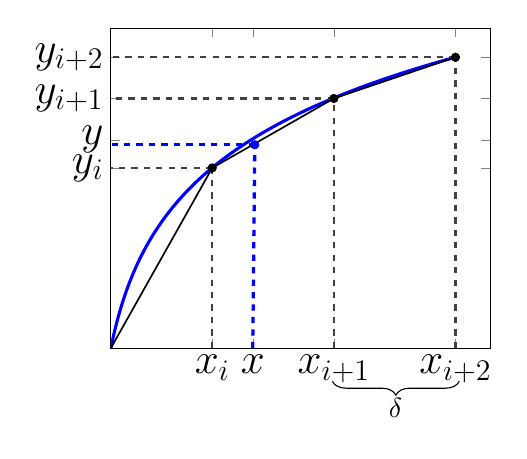
\begin{tikzpicture}[scale=0.75]
    \begin{axis}[
        width=8cm,
        height=7cm,
        xmin=1,
        ymin=0,
        %xmax=6.5,
        %ymax=5.5,
        xtick = {6,8,12,18},
        ytick = {1.79,2.07,2.48,2.89},
        xticklabels={\huge $x_i$,\huge $x$,\huge $x_{i+1}$,\huge$x_{i+2}$},
        yticklabels={\huge $y_i$ ,\huge $y$,\huge $y_{i+1}$,\huge$y_{i+2}$},
        ]

          \addplot[black,mark=none,line width=1.5pt,domain=1:18,samples=400,color=blue]  {ln(x)} node[above left,yshift=-0.5cm,xshift=-4.5cm] {};

      \addplot[only marks, black]  coordinates {(6,1.79) (12,2.48) (18,2.89)};
      \addplot[only marks, blue]  coordinates  {(8.1,2.02)};

      \draw[very thick, dashed,draw=black!75] (axis cs:6,0) -- (axis cs:6,1.79);
      \draw[very thick, dashed,draw=black!75] (axis cs:6,1.79) -- (axis cs:0,1.79);

      \draw[ultra thick, dashed,draw=blue] (axis cs:8,0) -- (axis cs:8.1,2.02);
      \draw[ultra thick, dashed,draw=blue] (axis cs:8.1,2.02) -- (axis cs:0,2.02);
          
      \draw[very thick, dashed,draw=black!75] (axis cs:12,0) -- (axis cs:12,2.48);
      \draw[very thick, dashed,draw=black!75] (axis cs:12,2.48) -- (axis cs:0,2.48);
          
      \draw[very thick, dashed,draw=black!75] (axis cs:18,0) -- (axis cs:18,2.89);
      \draw[very thick, dashed,draw=black!75] (axis cs:18,2.89) -- (axis cs:0,2.89);
          
      \draw[thick,draw=black] (axis cs:1,0) -- (axis cs:6,1.79);
      \draw[thick,draw=black] (axis cs:6,1.79) -- (axis cs:12,2.48);
      %\draw[thick,draw=black] (axis cs:8,2.07) -- (axis cs:12,2.48);                                                    
      \draw[thick,draw=black] (axis cs:12,2.48) -- (axis cs:18,2.89);                                                   
      
    \end{axis}

\draw [decorate,decoration={brace,amplitude=5pt,mirror,raise=4pt},yshift=0pt] (3.75,-0.375) -- (5.9,-0.375) node [black,midway,yshift=-0.5cm]{$\Spacing{}$};
  \end{tikzpicture}
  \caption{\label{fig:interpolation} Piecewise linear interpolation in between two breakpoints $x_i$ and $x_{i+1}$.}
\end{figure}


If $x_{i+1}-x_i$ is not constant $\forall i \in \{0,1,\hdots,k\}$, then the enclosing breakpoints can only be located by a search method. 
To this end, the number of comparisons performed grows with the number of breakpoints $k$. This can be avoided by even sampling of the interval $[\LowerBound, \UpperBound)$. Now, when defining a uniform spacing $\Spacing{ }=(x_{i+1}-x_i)>0$ between two breakpoints, it is possible to determine the index $\IndexLocation$ describing the interval $[\Breakpoint{i}, \Breakpoint{i+1})$ that includes $\Breakpoint{}$ as follows:
\begin{equation}\label{eq:even_space}
   \IndexLocation = \bigg\lfloor \frac{(\Breakpoint{}-\Breakpoint{0})}{\Spacing{ }}\bigg \rfloor
\end{equation}
Here, only the first value $\Breakpoint{0}$ and the spacing $\Spacing{ }$ are required to calculate $\IndexLocation$.
Finally, with $x_i = x_0 + i \cdot \delta$, \cref{eq:linEq} can be re-written to only use the points in $\SetRangeBreakpoints$, $\Breakpoint{0}$, the location $\IndexLocation$ according to \cref{eq:even_space} and the spacing $\Spacing{}$:
%
\begin{equation}\label{eq:2pt_line_even}
   \RangeBreakpoint{}=
   \RangeBreakpoint{i}+\frac{\Breakpoint{}-(\Breakpoint{0} + \IndexLocation \cdot \Spacing{})}{\Spacing{}}(\RangeBreakpoint{i+1}-\RangeBreakpoint{i})%& \text{if } \Breakpoint{0} \leq \Breakpoint{} \leq \Breakpoint{k}\\
\end{equation}
Thus, the function approximation can be achieved just by storing the $k+1$ range values of $X$. 
Henceforth, we only consider equidistant spacing between two breakpoints. 
The required memory footprint is referred to as $\MemF$ in the following sections.
For the above linear interpolation scheme, we obtain a memory footprint $\MemF$ of:
\begin{equation}
\MemF=k+1
\label{eq:refEquation}
\end{equation}

\section{Reference Approach}
\label{sec:reference}
In this section, we introduce the $\Reference$ approach~\cite{MATLAB:reference} used later (see \cref{sec:results}) for comparison.
According to \cref{eq:refEquation}, the memory footprint $\MemF$ is linear in $k$, the number of breakpoints.
An obvious remaining problem here is how to determine an equidistant spacing $\Spacing{ }$ being as large as possible such that still a user-given maximal approximation error bound $\AbsError$ is never exceeded for any evaluation of $\Fx$ inside the given interval $[\LowerBound, \UpperBound)$.
Let $p_i(x)$ denote the linear polynomial used to approximate the function $\Fx$ between the adjacent breakpoints $[\Breakpoint{i},\Breakpoint{i+1})$.
A two-point line expression can be derived from \cref{eq:linEq} as follows: 
\begin{equation}
p_i(x)=p_i(x_i)+\frac{x-x_i}{x_{i+1}-x_i}(p_i(x_{i+1})-p_i(x_i))
\label{eq:one}
\end{equation}
If the second derivative $f''(x)$ of $\Fx$ does exist at each point in $[x_i,x_{i+1})$, then the difference between the exact function value $\Fx$ and the value of the approximating polynomial $p_i(x)$ in $x_i \leq x < x_{i+1}$ is given as:
\begin{equation}
\Fx-p_i(x)=\frac{(x-x_i)(x-x_{i+1})}{2} f''(\varepsilon_x)
\label{eq:two}
\end{equation}
In \cref{eq:two}, $\varepsilon_x$ is some value between  $x_i$ and $x_{i+1}$.
In consequence, an error bound can be formulated based on \cref{eq:one,eq:two} as:
\begin{equation}
|\Fx-p_i(x)| \leq \frac{(x-x_i)(x_{i+1}-x)}{2} \max_{x_i\leq x < x_{i+1}} |f''(x)|
\label{eq:three}
\end{equation} 
With the spacing $\Spacing{i}=\Breakpoint{i+1}-\Breakpoint{i}$ between $\Breakpoint{i}$ and $\Breakpoint{i+1}$, the maximum value of $(x-x_i)(x_{i+1}-x)$ in \cref{eq:three} can be constrained as:
\begin{equation}\label{eq:four} 
\max_{x_i \leq x< x_{i+1}} (x-x_i)(x-x_{i+1}) = \frac{\Spacing{i}^2}{4}
\end{equation}
By combining \cref{eq:three,eq:four}, we obtain a maximum approximation error bound $E_i$ given a spacing $\Spacing{i}$:
\begin{equation}\label{eq:five}
E_i = \frac{\delta_i^2}{8} \max_{x_i\leq x < x_{i+1}} |f''(x)|
\end{equation}
The dependence of the approximation error on the second derivative of a function is intuitive from the perspective of linearity.
If $f$ is truly linear in the interval $[x_i,x_{i+1})$, then the second derivative vanishes implying an exact representation.
The value of $\underset{x_i\leq x <x_{i+1}}{\max} |f''(x)|$ can be expressed in closed form for elementary functions as well as some of the non-elementary functions due to their well-defined second derivatives.
Finally, for a given user-defined maximal approximation error bound $\AbsError$ to hold between any pair of breakpoints and assuming equi-distant spacings $\delta = \delta_i, 0 \leq i \leq k-1$, we can infer the biggest permissible spacing $\delta$ from the segment $i$ with the smallest value of $\Spacing{i}$ in \cref{eq:five}:
\begin{equation}\label{eq:spacing_err}
\delta(f,\AbsError,[\Breakpoint{0},\Breakpoint{k}))=\underset{0 \leq i \leq k-1}{\min} \bigg( 8\cdot \frac{\AbsError}{\underset{x_i\leq x < x_{i+1}}{\max} |f''(x)|} \bigg )^{\frac{1}{2}}
\end{equation}
\begin{figure}[t!]
	\centering
	\begin{subfigure}[b]{\textwidth}
		\centering
		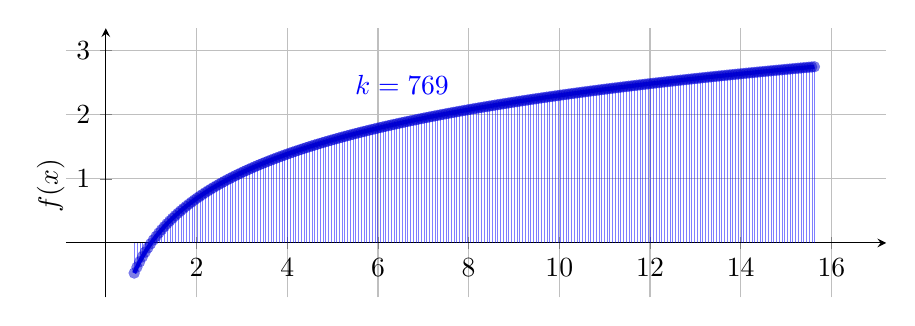
\begin{tikzpicture}[scale=1]
		\pgfplotsset{%compat=1.14,         
			width=12cm,     
			height=5cm, 
		}
		\begin{axis}[grid=both,
		ymin=-0.5,
		xmax=15.7,ymax=3,
		axis lines=middle,
		enlargelimits,
		ylabel=$f(x)$,
		ylabel style={rotate=90,xshift=-2cm,yshift=1cm},
		]
		\addplot+[ycomb,line width=0.05pt,domain=0.625:15.625,samples=250,opacity=0.5] {ln(x)};
		\addplot[black,mark=none,line width=1.5pt,domain=0.625:15.625,samples=400,color=blue]  {ln(x)} node[above left,yshift=-0.5cm,xshift=-4.5cm] {$k=769$};
		\end{axis}
		\end{tikzpicture}
		\caption{\label{fig:entries}Table-based approximation of $f(x)=log(x)$. Here, $\Spacing{}=0.019$, resulting in a memory footprint of $\MemF=k+1=770$ entries.}
	\end{subfigure}
	\begin{subfigure}[b]{\textwidth}
		\centering
		\begin{tikzpicture}[scale=1]
		\pgfplotsset{%compat=1.14,         
			width=12cm,     
			height=5cm, 
		}
		\begin{axis}[grid=both,
		axis lines=middle,
		enlargelimits,
		ylabel = $E$,
		ylabel style={rotate=90,xshift=-1.7cm,yshift=1cm,},
		%yshift=-1cm
		]
		\addplot[samples=16000,black,mark=none,line width=0.05pt,color=ao] table[x=x,y=y] {tikz/errormargins.dat};
		\draw[very thick, densely dashed,draw=red] (axis cs: 0,1.25E-4) --node[below,color=red]{\small $\AbsError$} (axis cs:15.625,1.25E-4);
		\end{axis}
		%\node[rotate=90] at (-0.5,1.5) {$E$};
		\end{tikzpicture} 
		\caption{\label{fig:ErrorMargin}Approximation Error obtained using \cref{eq:spacing_err} given $\AbsError=1.25E-04$.}
	\end{subfigure}
	\caption{\label{fig:tabApp} Function approximation of $\Fx=log(x)$ in the interval $[0.625,15.625)$. }
\end{figure}
E.g., \cref{fig:tabApp} illustrates the approximation of $\Fx=log(x)$ in the interval $[0.625,15.625)$ and $\AbsError=1.25E-04$.
This results in an spacing $\Spacing{}(log(x),\AbsError,[0.625,16.625))=0.019$.
From a spacing $\Spacing{}$ and the interval $[\LowerBound,\UpperBound)$, it is possible to generate the entries to be stored in a lookup table (see \cref{fig:entries}).
Given a spacing $\Spacing{}$  and an interval $[\LowerBound,\UpperBound)$, the memory footprint of this approach called $\Reference$ approach in the following can be calculated as:
\begin{equation}
\MemF^R(\Spacing{},[\LowerBound,\UpperBound)) = \bigg\lceil \dfrac{\UpperBound-\LowerBound}{\Spacing{}} \bigg\rceil + 1
\label{eq:six}
\end{equation}
Thus, the memory footprint of $\Fx=log(x)$, given the interval $[0.625,15.625)$, and $\Spacing{}=0.019$ is $\MemF^R(0.019,[0.626,15.625)) = 770$ entries.\\
The $\Reference$ approach performs the function approximation given a maximum approximation error $\AbsError$ by delivering a set of evenly spaced breakpoints.
However, this approach does not take into account the gradient in different regions of the interval.
This may result in an inefficient footprint, e.g., in \cref{fig:tabApp}, the interval closest to the left-most point $x_0=0.625$ determines the maximal spacing for the given approximation error $\AbsError$.
However, it can be seen that for larger values of $x$ (see \cref{fig:ErrorMargin}), a coarser spacing could be used when splitting the domain into sub-intervals and using different spacings $\delta_i$ within these.
Our main idea for the three proposed approaches introduced in the following is therefore to use different spacings $\delta_i$ by splitting the given interval into sub-intervals.

\section{Interval Splitting Algorithms}
\label{sec:proposed}
Uniform spacing schemes such as even spacing (see the $\Reference$ approach in \cref{sec:reference}) or power of two spacing do not consider the local variation of many functions in the interval of approximation.
This section introduces three algorithmic approaches to  partition a given interval $[\LowerBound,\UpperBound)$ into a set of non-uniform sub-intervals and determine a uniform spacing of breakpoints in each sub-interval given a maximum tolerable approximation error $\AbsError$.
The proposed algorithms perform the segmentation of the interval $[\LowerBound,\UpperBound)$ into a partition of sub-intervals exploiting the granularity in the spacing according to the steepness of a given function.
Here, we trade between the number of generated sub-intervals and the memory footprint reduction.
%The presented algorithms differ mainly in the way the sub-interval partitions are computed. 
The presented algorithms differ mainly in the heuristic proposed to compute the set of sub-interval partitions.
The first two algorithms (\cref{alg:alg1,alg:alg2}) split a given interval $[\LowerBound,\UpperBound)$ into two sub-intervals recursively until a corresponding stopping criterion is satisfied. 
\cref{alg:alg1}, called $\Binary$ always splits a sub-interval at the midpoint.
In contrast, \cref{alg:alg2}, called $\Hierarchical$ finds the best splitting point by sweeping over the given interval such that the reduction in memory footprint $\MemF$ when splitting is maximized. 
Here, the step size for the sweep is given as an input.
Finally, \cref{alg:alg3} named $\Sequential$ also performs a sweep-based interval splitting. 
However here, interval splitting is performed in a single sweep over the overall interval $[\LowerBound,\UpperBound)$.
%The third and last approach (\cref{alg:alg3}) named $\Sequential$ also sweeps over the given interval until the sweep value becomes equal to the upper bound of the interval. 
%However, the latter approach is iterative and produces the set of sub-intervals after a single sweep. This algorithm will be called $sequential segmentation$. Common to all three $proposed$ approaches is that a splitting point is accepted or rejected based on a given threshold.  
\newlength{\commentWidth}
\setlength{\commentWidth}{7cm}
\newcommand{\atcp}[1]{\tcp*[r]{\makebox[\commentWidth]{#1\hfill}}}
\begin{algorithm}[t]
	\small
	\SetAlgoLined
	\SetKwFunction{InsertPartition}{Binary}
	\SetKwFunction{FMain}{Binary}
	\SetKwProg{Fn}{Function}{}{}
	\Fn{\FMain{$\ReductionThreshold$,$\AbsError$,$f$,$\Partition{i}$,$\Partition{i+1}$}}{
		
		\SetKwInOut{Input}{Inputs}\SetKwInOut{Output}{Outputs}
			\KwIn{$f$ is the function to be approximated\\
			\hspace{10mm}$\Partition{i}$ is the lower bound of the interval\\
			\hspace{10mm}$\Partition{i+1}$ is the upper bound of the interval\\
			\hspace{10mm}$\ReductionThreshold$ is the reduction threshold (0,1] \\
			\hspace{10mm}$\AbsError$ is the maximum approximation error\\
		}
		\KwOut{$\SetPartitions=\{\Partition{0}, \Partition{1}, \ldots, \Partition{n}  \}$ is the set of sub-interval boundaries\\
			
		}
		\Begin{
			
			$\SetPartitions \leftarrow \{\Partition{i},\Partition{i+1}\} $\tcp*[f]{\footnotesize Initial set of sub-intervals boundaries} \\  
			$\Spacing{p} \leftarrow \delta(f,\AbsError,[\Partition{i}, \Partition{i+1}))$ \tcp*[f]{\footnotesize Calculate the spacing in the interval} \\
			$\NBreakpoints{p}\leftarrow \MemF(\Spacing{p},[\Partition{i}, \Partition{i+1}))$ \tcp*[f]{\footnotesize Calculate the $\MemF$ of the interval} \\
			
			$bp \leftarrow \dfrac{\Partition{i} + \Partition{i+1}}{2}$ \tcp*[f]{\footnotesize Midpoint between $\Partition{i}$ and $\Partition{i+1}$} \\
			
			
			$\Spacing{bp_1} \leftarrow \delta(f,\AbsError,[\Partition{i}, bp))$ \tcp*[f]{\footnotesize Calculate the spacing of sub-intervals} \\
			$\Spacing{bp_2} \leftarrow \delta(f,\AbsError,[bp,\Partition{i+1}))$ \\ %\tcp*[f]{\footnotesize sub-intervals} \\
			
			\If{$\Spacing{bp_1} \neq  \Spacing{bp_2} $}
			{
				$\NBreakpoints{bp_1}\leftarrow \MemF(\Spacing{bp_1},[\Partition{i}, bp))$ \tcp*[f]{\footnotesize Calculate the $\MemF$ of sub-intervals}  \\
				$\NBreakpoints{bp_2}\leftarrow \MemF(\Spacing{bp_2},[bp, \Partition{i+1}))$ \\ %\tcp*[f]{\footnotesize sub-intervals} \\
				\If(\tcp*[f]{\footnotesize If \textbf{true}, accept sub-interval split}){ $\NBreakpoints{bp_1}+\NBreakpoints{bp_2}  < \NBreakpoints{p}  \cdot \ReductionThreshold$}{
					\vspace{0.2cm}
					$\SetPartitions \leftarrow \{\InsertPartition(\ReductionThreshold,\AbsError,f,\Partition{i},bp) \cup \InsertPartition(\ReductionThreshold,\AbsError,f,bp,\Partition{i+1}) \}$ \\
					\tcp*[f]{\footnotesize Recursive call for sub-intervals $[\Partition{i},bp)$ and $[bp,\Partition{i+1})$}
				}
				%{}
				%{	\textbf{return} $ \SetPartitions $ \\}
			}
			\textbf{return} $ \SetPartitions $ \\	
			
		}	
		
	}
	\textbf{End Function}
	\caption{\small Binary Interval Splitting $[\Partition{i}, \Partition{i+1})$}\label{alg:alg1}
	%	\vspace{-0.5cm}
\end{algorithm}
\subsection{Binary Segmentation}\label{bin_seg}
\cref{alg:alg1} performs a $\Binary$ of a given interval $[\Partition{i}, \Partition{i+1})$ in which the function $\Fx$ is to be approximated. 
The inputs of \cref{alg:alg1} are the function $\Fx$, the interval $\Interval$, the maximum approximation error $\AbsError$ and a threshold value $\ReductionThreshold$ which determines whether a new sub-interval split is accepted.
\textit{Binary segmentation} determines a partition $\SetPartitions$ of sub-intervals, from which a set of spacings $\SetSpacings$ and a set $\SetNBreakpoints$ containing the numbers of breakpoints in each sub-interval can be obtained.
Each element of $\Partition{i} \in \SetPartitions$  represents a left (sub-interval) delimiter value. The number of sub-intervals is thus $|\SetPartitions|-1$.
As an example for illustration, assume Algorithm 1 determines the sub-interval splitting $\SetPartitions=\{\Partition{0}, \Partition{1}, \Partition{2}\}$ for a given function, that yields the sets of values $\SetSpacings=\{\Spacing{0},\Spacing{1}\}$ and $\SetNBreakpoints=\{\NBreakpoints{0},\NBreakpoints{1}\}$.
$P$ represents a partitioning of a given interval into two sub-intervals
$[\Partition{0},\Partition{1})$ and $[\Partition{1},\Partition{2})$.
Here, $\Spacing{0}$ and $\NBreakpoints{0}$ correspond to the spacing and the number of breakpoints for the sub-interval $[\Partition{0},\Partition{1})$ as well as $\Spacing{1}$ and $\NBreakpoints{1}$ correspond to sub-interval $[\Partition{1},\Partition{2})$.
The memory footprint corresponding to $P$ is therefore given by:
\begin{equation}
\MemF^P([\Partition{0},\Partition{|\SetPartitions|-1})) = \sum^{|\SetPartitions|-1}_{j=0} \NBreakpoints{j}
\label{eq:memFProposed}
\end{equation}
\textit{Binary segmentation} is a recursive algorithm, which evaluates the reduction in $\MemF$ obtained by splitting the current interval $[\Partition{i},\Partition{i+1})$ at the midpoint $bp$. 
Initially, the lower and upper bounds of the interval of approximation ($\Interval$) are provided as the inputs $\Partition{i}=\LowerBound$ and $\Partition{i+1}=\UpperBound$ to the function $Binary$. 
The first step is to initialize $\SetPartitions$ as $\{\Partition{i}, \Partition{i+1}\}$ (see Line $4$ in \cref{alg:alg1}). 
The spacing $\Spacing{p}$ and the number of breakpoints $\NBreakpoints{p}$ are obtained using the $\Reference$ approach in the interval $[\Partition{i}, \Partition{i+1})$ (see \cref{sec:reference}).\\
The midpoint $bp$ of the input interval is used to create the left sub-interval $bp_1=[\Partition{i},bp)$ and right sub-interval $bp_2=[bp,\Partition{i+1})$. 
The spacings $\delta_{bp_1}$ and $\delta_{bp_2}$, and the number of breakpoints $\NBreakpoints{bp_1}$ and $\NBreakpoints{bp_2}$ of sub-intervals $bp_1$ and $bp_2$ are then calculated according to \cref{eq:spacing_err} and \cref{eq:six} (see Lines 8-12 in \cref{alg:alg1}). 
If the sum of $\NBreakpoints{bp_1}$ and $\NBreakpoints{bp_2}$ denoting the memory footprints of $bp_1$ and $bp_2$ is less than a specified fraction (threshold $\ReductionThreshold$) of $\NBreakpoints{p}$ (see Line 13 in \cref{alg:alg1}), the memory footprint reduction and thus split are accepted and the $binary$ function is called recursively for the sub-intervals $bp_1$ and $bp_2$, respectively.
Otherwise, the algorithm terminates and returns the current input interval boundaries ($\{p_i, p_{i+1}\}$).
The final set $P$ returned is the union of all the returned sub-intervals. 
\begin{figure}[t!]
	\centering
	\begin{subfigure}[b]{\textwidth}
		\centering
		\begin{tikzpicture}[scale=1]
		\pgfplotsset{%compat=1.14,         
			width=10cm,     
			height=5cm, 
		}
		\begin{axis}[grid=both,
		ymin=-0.5,
		xmax=15.7,ymax=3,
		axis lines=middle,
		enlargelimits
		]
		
		\addplot+[ycomb,blue,line width=0.1pt,domain=0.625:2.5,samples=95,opacity=0.5] {ln(x)};  
		\addplot+[ycomb,blue,line width=0.1pt,domain=2.5:4.375,samples=27,opacity=0.5,mark=o] {ln(x)};  
		\addplot+[ycomb,blue,line width=0.1pt,domain=4.375:8.125,samples=29,opacity=0.5,mark=o] {ln(x)};  
		\addplot+[ycomb,blue,line width=0.1pt,domain=8.125:15.625,samples=31,opacity=0.5,mark=o] {ln(x)};   
		
		\addplot[black,mark=none,line width=0.5pt,domain=0.625:15.625,samples=400,color=ao]  {ln(x)} node[above left,yshift=-0.5cm,xshift=-4.5cm] {$\sum \kappa_j=182$}; 
		
		\draw[very thick, densely dashed,draw=red] (axis cs: 0.625,0) -- (axis cs:0.625,4);
		\draw[very thick, densely dashed,draw=red] (axis cs: 2.5,0) -- (axis cs:2.5,4);
		\draw[very thick, densely dashed,draw=red] (axis cs:4.375,0) -- (axis cs:4.375,4);
		\draw[very thick, densely dashed,draw=red] (axis cs:8.125,0) -- (axis cs:8.125,4);
		\draw[very thick, densely dashed,draw=red] (axis cs:15.625,0) -- (axis cs:15.625,4);
		\end{axis}
		\node at (0.8,3.80) {$\Partition{0}$};
		\node at (1.6,3.80) {$\Partition{1}$};
		\node at (2.4,3.80) {$\Partition{2}$};
		\node at (4.2,3.80) {$\Partition{3}$};
		\node at (7.7,3.80) {$\Partition{4}$};
		
		\draw [decorate,decoration={brace,amplitude=5pt,mirror,raise=4pt},yshift=0pt] (0.66,0.1) -- (1.6,0.1) node [black,midway,xshift=-0.4cm,yshift=-0.75cm]{\begin{tabular}{c} $\Spacing{0}=0.02$ \\ $\NBreakpoints{0}=97$  \end{tabular}};
		\draw [decorate,decoration={brace,amplitude=5pt,mirror,raise=4pt},yshift=0pt] (1.6,0.1) -- (2.45,0.1) node [black,midway,xshift=0.1cm,yshift=-0.75cm]{\begin{tabular}{c} $\Spacing{1}=0.08$ \\ $\NBreakpoints{1}=25$  \end{tabular}};
		\draw [decorate,decoration={brace,amplitude=5pt,mirror,raise=4pt},yshift=0pt] (2.45,0.1) -- (4.2,0.1) node [black,midway,xshift=0.3cm,yshift=-0.75cm] {\begin{tabular}{c} $\Spacing{2}=0.14$ \\ $\NBreakpoints{2}=29$  \end{tabular}};
		\draw [decorate,decoration={brace,amplitude=5pt,mirror,raise=4pt},yshift=0pt] (4.2,0.1) -- (7.7,0.1) node [black,midway,xshift=0cm,yshift=-0.75cm] {\begin{tabular}{c} $\Spacing{3}=0.26$ \\ $\NBreakpoints{3}=31$  \end{tabular}};
		\end{tikzpicture}
		\caption{\label{fig:samples}Function approximation of $log(x)$ obtained by $\Binary$.}
	\end{subfigure}
	\begin{subfigure}[b]{\textwidth}
		\centering
		\begin{tikzpicture}[scale=0.45]
		\ErrorPlots%\right) 
		\end{tikzpicture}
		\caption{\label{fig:proposedError}Error margins obtained by \Binary.}
	\end{subfigure}
	\caption{\label{fig:proposed} For a user-given maximal approximation error bound of $\AbsError=1.22E-04$, the algorithm $\Binary$ identifies the partition $\SetPartitions=\{0.625,2.5,4.375,8.125,15.625\}$ for splitting threshold $\ReductionThreshold=0.3$ describing four sub-intervals $[0.625,2.5)$, $[2.5,4.375)$, $[4.375,8.125)$ and $[8.125,15.625)$.
		Here, a total of $\MemF = 182$ entries represents an overall reduction in memory footprint of $76\,\%$ compared to the $\Reference$ approach (see \cref{fig:entries}).
	}
	%\vspace{-0.5cm}
\end{figure}
The value $\ReductionThreshold \in (0,1]$ indicates the threshold of an acceptable memory footprint reduction. 
E.g., $\ReductionThreshold=0.3$ indicates that an interval split must lead to a footprint reduction of at least $30\,\%$ of the given interval in order to continue splitting the left and right sub-intervals.\\
\cref{fig:proposed} illustrates the proposed recursive sub-interval splitting approximation method using as an example, the function $f=log(x)$ to be approximated in the interval $[p_i,p_{i+1})=[0.625,15.625)$ with a maximum approximation error of $\AbsError=1.22E-04$ and splitting threshold $\ReductionThreshold=0.3$. 
To find a partition of the interval, $\Binary$ is performed with the inputs $\ReductionThreshold$, $\AbsError$, $f$ and $[p_i,p_{i+1})$.
Using the $\Reference$ approach, the uniform spacing $\Spacing{p}$ and memory footprint $\MemF$ are obtained as $\Spacing{p}=0.019$ and $\MemF=770$, respectively.
%At this point, the set of partitions $\SetPartitions=\{0.625,15.625\}$, the set of spacings $\SetSpacings=\{0.019\}$ and the list of breakpoint numbers is $\SetNBreakpoints=\{770\}$.
When applying \cref{alg:alg1}, the middle point $bp=8.125$ of the interval $[0.625,15.625)$ is determined first.
The left and right sub-intervals are derived using $bp$, thus $bp_1=[0.625,8.125)$ and $bp_2=[8.125,15.625)$.
After calculating the spacing $\Spacing{bp_1}=0.0195$ and $\Spacing{bp_2}=0.25$ for these two sub-intervals, respectively, the number of breakpoints results in $\NBreakpoints{bp_1}=384$ and $\NBreakpoints{bp_2}=31$.
The new partition has a memory footprint of $\MemF^P=(384+31) = 415$.
Compared to the memory footprint of 770, the achieved reduction is $46\,\%$ which is greater than the required threshold of $30\,\%$ ($\ReductionThreshold=0.3$).
Then, the function $binary$ is called recursively for the accepted right and left sub-intervals $[0.625,8.125)$ and $[8.125,15.625)$, respectively.
%Thus $InsertPartition$ is performed again with  $[0.625,8.125)$ and  $[8.125,15.625)$ as input intervals.
The previous is repeated until no more splittings can be achieved with an acceptable memory footprint reduction.
\cref{alg:alg1} stops with the final partition $\SetPartitions=\{0.625,2.5,4.375,8.125,15.625\}$.
Hence, four sub-intervals $[0.0625,2.5)$, $[2.5,4.375)$, $[4.375,8.125)$, and $[8.125,15.625)$ were identified (see \cref{fig:proposed}).
The spacings and the number of breakpoints of each sub-intervals are $\SetSpacings=\{0.02,0.08,0.13,0.25\}$ and $\SetNBreakpoints=\{97,25,29,31\}$.
From the set of memory footprints $\SetNBreakpoints$, the overall memory footprint $\MemF^P([0.625,15.625))=(97+25+29+31)=182$ is calculated.
Compared to the reported memory footprint $\MemF^R=770$ for the same function, interval, and error bound (see \cref{fig:tabApp}) using the $\Reference$ approach, $\Binary$ is thus able to reduce the memory footprint by $76\,\%$ while respecting the maximum approximation error bound imposed by the given $\AbsError$ (see \cref{fig:proposedError}).\\
However, using the midpoint in the partitioning heuristic might lead to a sub-optimal exploration of the partitions in approximation of a given function $f(x)$. The next section introduces an alternative recursive approach which employs a different heuristic in attempt to achieve even larger memory footprint reductions.
\subsection{Hierarchical Segmentation}\label{hier_seg}
\textit{Hierarchical segmentation} is an alternative recursive interval splitting heuristic described by the function $Hierarchical$ in \cref{alg:alg2}. 
For each candidate interval $[\Partition{i},\Partition{i+1})$, a linear sweep is performed instead of just using the midpoint to split the interval.
\textit{Hierarchical segmentation} then chooses the splitting point $sp$ with the highest memory footprint reduction and performs a split at $sp$, if the reduction is acceptable.
In order to reduce the computational effort, a step size $\StepSize$ denotes the uniform distance between two adjacent splitting point candidates.
The value of $\StepSize$, the function $f$, the interval $[\Partition{i},\Partition{i+1})$, the reduction threshold $\ReductionThreshold$, and the maximum approximation error $\AbsError$ are passed as inputs to \cref{alg:alg2} (see Line 2 of \cref{alg:alg2}).
The output is the set $\SetPartitions$, from which a set of spacings $\SetSpacings$ and a set of number of breakpoints $\SetNBreakpoints$ are determined (see Line 3 of \cref{alg:alg2}).\\
Similar to \cref{alg:alg1}, \cref{alg:alg2} initializes the set $\SetPartitions=\{\Partition{i},\Partition{i+1}\}$ with the lower and upper bounds of a given input interval $[\Partition{i},\Partition{i+1})$ (see Line 4 in \cref{alg:alg2}).
The algorithm then computes the maximal number of splitting point candidates $j_{max}$ based on the step size $\StepSize$ as a parameter (see Line 5 in \cref{alg:alg2}). 
In the next step, we evaluate all the possible memory footprints by splitting the input interval at each candidate point. 
The splitting point $sp$ is then chosen as the point delivering the smallest memory footprint (see Lines 6 and 7 in \cref{alg:alg2}).
The left and right sub-intervals are derived as $sp_1=[\Partition{i},sp)$ and $sp_2=[sp,\Partition{i+1})$, respectively.
The spacings $\Spacing{sp_1}$ and $\Spacing{sp_2}$ and number of breakpoints $\NBreakpoints{sp_1}$ and $\NBreakpoints{sp_2}$ of sub-intervals $sp_1$ and $sp_2$ are calculated using the $\Reference$ approach (see Lines 9-12 in \cref{alg:alg2}). 
If the sum of $\NBreakpoints{sp_1}$ and $\NBreakpoints{sp_2}$ denoting the memory footprint of an interval split at the position $sp$ is less than a specified fraction $\ReductionThreshold$ of $\NBreakpoints{p}$ (the memory footprint over the interval $[\Partition{i},\Partition{i+1})$), the split is accepted and the hierarchical function is called recursively to explore the right and left sub-intervals (see Line 13 in \cref{alg:alg2}).
\begin{algorithm}[t!]
	\small
	\SetAlgoLined
	\SetKwFunction{Hierarchical}{Hierarchical}
	\SetKwFunction{FMain}{Hierarchical}
	\SetKwProg{Fn}{Function}{}{}
	\Fn{\FMain{$\ReductionThreshold$,$\AbsError$,$f$,$\Partition{i}$,$\Partition{i+1}$}}{
		%\SetKwInOut{Input}{Inputs}\SetKwInOut{Output}{Outputs}
			\KwIn{$f$ is the function to be approximated\\
			\hspace{10mm}$\Partition{i}$ is the lower bound of the interval\\
			\hspace{10mm}$\Partition{i+1}$ is the upper bound of the interval\\
			\hspace{10mm}$\ReductionThreshold$ is the reduction threshold (0,1] \\
			\hspace{10mm}$\AbsError$ is the maximum approximation error\\
			\hspace{10mm}$\StepSize$ is the sweep step size\\
		}
		\KwOut{$\SetPartitions=\{\Partition{0}, \Partition{1}, \ldots, \Partition{n}  \}$ is set of sub-interval boundaries\\
			
		}
		\Begin{
			
			$\SetPartitions \leftarrow \{\Partition{i},\Partition{i+1}\} $\tcp*[f]{\footnotesize Initial set of sub-intervals boundaries} \\  
			$j_{max} \leftarrow  \bigg\lfloor{\dfrac{\Partition{i+1} - \Partition{i}}{\varepsilon}} \bigg\rfloor$ \tcp*[f]{\footnotesize Calculate the number of splitting point candidates} \\
			{\scriptsize $j^* \leftarrow \underset{1\leq j \leq j_{max}}{\operatorname{arg\hspace{1mm}min}}\MemF(\delta(f,\AbsError,[\Partition{i},\Partition{i}+j\times \StepSize)),[\Partition{i},\Partition{i}+j\times\StepSize)) + \MemF(\delta(f,\AbsError,[\Partition{i}+j\times\StepSize,\Partition{i+1})),[\Partition{i}+j\times\StepSize,\Partition{i+1}))$} \\
			%			$\begin{aligned}
			%			j^* \leftarrow \underset{1\leq j \leq j_{max}}{\operatorname{arg\hspace{1mm}min}}\MemF(\delta(f,\AbsError,[\Partition{i}, \Partition{i}&+j\times \varepsilon]),[\Partition{i}, \Partition{i}+j\times \varepsilon]) +\\
			%			&+ \MemF(\delta(f,\AbsError,[\Partition{i}+j\times \varepsilon,\Partition{i+1}]),[\Partition{i}+j\times \varepsilon,\Partition{i+1}]) 	
			%			\end{aligned}$
			$sp \leftarrow \Partition{i}+j^*\times \varepsilon$ \tcp*[f]{\footnotesize Determine the splitting point} \\
			$\NBreakpoints{p}\leftarrow \MemF(\Spacing{p},[\Partition{i}, \Partition{i+1}))$ \tcp*[f]{\footnotesize Calculate the $\MemF$ of the interval} \\
			
			$\Spacing{sp_1} \leftarrow \delta(f,\AbsError,[\Partition{i}, sp))$ \tcp*[f]{\footnotesize Calculate the spacing of sub-intervals} \\
			$\Spacing{sp_2} \leftarrow \delta(f,\AbsError,[sp,\Partition{i+1}))$\\
			%\If{$\Spacing{sp_1} \neq  \Spacing{sp_2} $}
			%{
			$\NBreakpoints{sp_1}\leftarrow \MemF(\Spacing{sp_1},[\Partition{i}, sp))$ \tcp*[f]{\footnotesize Calculate the $\MemF$ of sub-intervals}  \\
			$\NBreakpoints{sp_2}\leftarrow \MemF(\Spacing{sp_2},[sp, \Partition{i+1}))$ \\
			
			\If(\tcp*[f]{\footnotesize If \textbf{true}, accept interval split}){ $\NBreakpoints{sp_1}+\NBreakpoints{sp_2}  < \NBreakpoints{p}  \cdot \ReductionThreshold$}{
				\vspace{0.2cm}
				%$\SetPartitions \leftarrow$ \{\InsertPartition{$\ReductionThreshold$,$\AbsError$,$f$,$\Partition{i}$,$sp$,$\varepsilon$} \InsertPartition{$\ReductionThreshold$,$\AbsError$,$f$,$sp$,$\Partition{i+1}$}\}\\ \tcp*[f]{\footnotesize Updating $\SetPartitions$}\\
				$\SetPartitions \leftarrow \{\Hierarchical(\ReductionThreshold,\AbsError,f,\Partition{i},sp,\varepsilon) \cup \Hierarchical(\ReductionThreshold,\AbsError,f,sp,\Partition{i+1},\varepsilon) \}$\\ \tcp*[f]{\footnotesize Recursive call for sub-intervals $[\Partition{i},sp)$ and $[sp,\Partition{i+1})$}\\
				
			}
			{\textbf{return} $ \SetPartitions $ }
			%}
		}	
	}
	\textbf{End Function}
	\caption{\small  Hierarchical Interval Splitting $[\Partition{i}, \Partition{i+1})$}\label{alg:alg2}
\end{algorithm}
Otherwise, the algorithm terminates returning the current upper and lower interval bounds (see Line 16 in \cref{alg:alg2}). 
The final set $\SetPartitions$ is then returned as the union of split intervals.\\
\cref{fig:hierarchical} shows the hierarchical segmentation approach over the interval $[\Partition{i},\Partition{i+1})=[0.625,15.625)$.
E.g., let $f(x)=log(x)$, the reduction threshold $\ReductionThreshold=0.3$, the maximum absolute error $\AbsError=1.22E-04$, and the sweep size $\StepSize=0.015$.
At this point, the number of candidate splitting points is $j_{max}=\frac{15.625-0.625}{0.015}=1000$.
This set of points can be expressed in terms of $\StepSize$ and $j_{max}$ as $\{\Partition{i}+j\cdot\StepSize|i\leq j<j_{max}\}$.
After evaluating each candidate, \cref{alg:alg2} determines $sp=2.90$ as the best candidate resulting in the left sub-interval $sp_1=[0.625,2.90)$ and the right sub-interval $sp_2=[2.90,15.625)$. 
$\NBreakpoints{sp_1}$ is equal to 117 and $\NBreakpoints{sp_2}$ is 141.
The partition has a memory footprint of $\NBreakpoints{sp_1}+\NBreakpoints{sp_2}=(117+141)=258$ which implies a $66.5\,\%$ reduction in memory footprint compared to $\MemF^R$ obtained by the $\Reference$ approach. 
The achieved reduction is greater than the required threshold reduction of $30\,\%$ ($\ReductionThreshold=0.3$).
Thus, the recursive splitting continues for the sub-intervals $sp_1$ and $sp_2$.
The previous steps are repeated until no more splitting can be performed resulting in the set $\SetPartitions=\{0.6250,1.2106,2.9073,6.2556,15.6250\}$, as illustrated in \cref{fig:hierarchical} where the set of spacings $\SetSpacings=\{0.01,0.06,0.09,0.19\}$, and the set of breakpoints $\SetNBreakpoints=\{30,25,37,49\}$.
The value of $\MemF^P([0.625,15.625))=30+45+37+49=161$. 
Hierarchical segmentation is able to reduce the memory footprint by $79\,\%$ with respect to $\Reference$ approach and by $11.5\,\%$ compared to binary segmentation (\cref{alg:alg1}).
%It is important to note here that the difference between the reductions produced by the previously proposed methods decreases with increase in number of sub-intervals.
\begin{algorithm}[t]
	\small
	\SetAlgoLined
	\SetKwFunction{Sequential}{Sequential}
	\SetKwFunction{FMain}{Sequential}
	\SetKwProg{Fn}{Function}{}{}
	\Fn{\FMain{$\ReductionThreshold$,$\AbsError$,$f$,$\LowerBound$,$\UpperBound$}}{
		
		\SetKwInOut{Input}{Inputs}\SetKwInOut{Output}{Outputs}
		\KwIn{$f$ is the function to be approximated\\
			\hspace{10mm}$\LowerBound$ is the lower bound of the interval\\
			\hspace{10mm}$\UpperBound$ is the upper bound of the interval\\
			\hspace{10mm}$\ReductionThreshold$ is the reduction threshold (0,1]\\
			\hspace{10mm}$\AbsError$ is the maximum approximation error\\
			\hspace{10mm}$\varepsilon$ is the sweep step size\\
		}
		\KwOut{$\SetPartitions=\{\Partition{0}, \Partition{1}, \ldots, \Partition{n}  \}$ is the set of sub-interval boundaries\\
			
		}
		\vspace{0.2cm}
		$\SetPartitions \leftarrow \{\LowerBound\}$ \tcp*[f]{\footnotesize Initialize $P$ with the lower bound of the interval} \\  
		$x_p\leftarrow x_0$ \\%\tcp*[f]{\footnotesize the last element of $P$} \\
		$i_{max} \leftarrow  \bigg\lfloor{\dfrac{a}{\varepsilon}} \bigg\rfloor$ \tcp*[f]{\footnotesize Calculate the number of splitting point candidates} \\
		$\Spacing{p} \leftarrow \delta(f,\AbsError,[x_p,\UpperBound))$ \tcp*[f]{\footnotesize Calculate the spacing of sub-interval $[x_p,\UpperBound]$} \\
		$\NBreakpoints{p}\leftarrow \MemF(\Spacing{p},[x_p,x_0+a))$ \tcp*[f]{\footnotesize Calculate the $\MemF$ of sub-interval $[x_p,\UpperBound]$} \\
		\For{$i\leftarrow 1$ \KwTo $i_{max}$}{\label{forins}
			$sp \leftarrow x_0+i\cdot\varepsilon$\tcp*[f]{\footnotesize Determine the splitting point}\\
			\vspace{0.1cm}
			$\Spacing{sp_1} \leftarrow \delta(f,\AbsError,[x_p,sp))$ \tcp*[f]{\footnotesize Calculate the spacing of sub-intervals} \\
			$\Spacing{sp_2} \leftarrow \delta(f,\AbsError,[sp,x_0+a))$ \\
			
			$\NBreakpoints{sp_1}\leftarrow \MemF(\Spacing{sp_1},[x_p,sp))$ \tcp*[f]{\footnotesize Calculate the $\MemF$ of sub-intervals}  \\
			$\NBreakpoints{sp_2}\leftarrow \MemF(\Spacing{sp_2},[sp,x_0+a))$ \\
			
			\If(\tcp*[f]{\footnotesize If \textbf{true}, accept the interval split}){ $\NBreakpoints{sp_1}+\NBreakpoints{sp_2}  < \NBreakpoints{\Partition{}}  \cdot \ReductionThreshold$}{
				$\SetPartitions \leftarrow \SetPartitions \cup \{sp\}$ \tcp*[f]{\footnotesize Updating $\SetPartitions$}\\
				$x_p\leftarrow sp$ \tcp*[f]{\footnotesize Updating $x_p$} \\
				$\Spacing{p} \leftarrow \delta(f,\AbsError,[x_p,x_0+a))$ \tcp*[f]{\footnotesize Calc. the spacing} \\
				$\NBreakpoints{p}\leftarrow \MemF(\Spacing{p},[x_p,x_0+a))$ \tcp*[f]{\footnotesize Calc. the $\MemF$ of the interval to split} \\
			}
			
		}
		$\SetPartitions \leftarrow \SetPartitions \cup \{x_0+a\}$ \tcp*[f]{\footnotesize Updating $P$ with the upper bound of the interval} \\  
	}	
	\textbf{End Function}
	\caption{\small Sequential Interval Splitting $[\LowerBound,\UpperBound)$}\label{alg:alg3}
\end{algorithm}
\subsection{Sequential Segmentation} 
%The third presented approach is called \textit{sequential segmentation}, which performs a linear sweep of the input interval as the \textit{hierarchical segmentation} (see \cref{alg:alg2}).
\cref{alg:alg3} describes the third approach called \textit{sequential segmentation} and receives as inputs also the function $\Fx$ to approximate, the interval $[\LowerBound, \UpperBound)$, maximum approximation error $\AbsError$, the reduction threshold $\ReductionThreshold$ and a sweep step size $\varepsilon$.
Sequential segmentation performs a linear sweep of the overall input interval similar to the hierarchical segmentation.
However, it produces a partition $P$ of a given interval $[\LowerBound, \UpperBound)$ iteratively in a single sweep.
The set of splitting point candidates can be represented as $\{sp \hspace{1mm}|\hspace{1mm}sp=x_0 + i \cdot \varepsilon\}$ where $1\leq i < i_{max}$.
Here, the distance between two adjacent points in the set is $\StepSize$ and the number of candidates $i_{max}$ is determined based on the length of interval $a$ and the step size $\varepsilon$ (see Line 2 in \cref{alg:alg3}).\\
\cref{alg:alg3} initializes $P$ and $x_p$ with the lower bound $x_0$ of the input interval (see Lines 1-2 in \cref{alg:alg3}).
The value of $x_p$ always corresponds to the last entry of the set of partitions $P$. 
The spacing $\Spacing{p}$ and the memory footprint $\NBreakpoints{p}$ of the input interval $\Interval$ are calculated following the $\Reference$ approach (\cref{sec:reference}).
The algorithm iterates through the sweep candidates $sp$ and calculates the memory footprints $\NBreakpoints{sp_1}$ and $\NBreakpoints{sp_2}$ of the sub-intervals $sp_1=[x_p,sp)$ and $sp_2=[sp,x_0+a)$, respectively.
If the memory footprint of the input interval $[\LowerBound, \UpperBound)$ split at $sp$ is less than a fraction $\ReductionThreshold$ of $\NBreakpoints{p}$, then the set $\SetPartitions$ is updated with $sp$ as a new splitting point.
%If the reduction in $M_f$ after splitting exceeds $\ReductionThreshold$ i.e. $\NBreakpoints{sp_1}+\NBreakpoints{sp_2} < \ReductionThreshold \cdot \NBreakpoints{p}$, then $P$ is updated with $sp$ as a splitting point.
The values $x_p$, $\Spacing{p}$ and $\NBreakpoints{p}$ are updated accordingly (see Lines 13-16 in \cref{alg:alg3}).
\cref{alg:alg3} stops with the last sweep value which is one step size smaller than $x_0+a$.\\
The main difference between \textit{sequential segmentation} and \textit{binary} as well as \textit{hierarchical segmentation} is how the partition points are generated. 
Here, \textit{sequential segmentation} sweeps from left to right to find the set of partitions, and only one iteration over the given interval is required.
In contrast, \textit{binary} and \textit{hierarchical} perform a recursive exploration of each split interval. 
Every time a new partition point is found, two new sub-intervals located at the right and the left are generated and explored until no more acceptable memory footprint reductions are achieved. \\
\cref{fig:sequential} presents the partition obtained by the algorithm \textit{sequential segmentation} for $f(x)=log(x)$, over the interval $[0.625,15.625)$, the reduction threshold $\ReductionThreshold=0.3$, maximum absolute error $\AbsError=1.22E-04$, and the sweep size $\StepSize=0.3$.
\begin{figure}[t!]
	\centering
	\begin{subfigure}[b]{0.45\textwidth}
		\centering
		\resizebox{\textwidth}{!}{
			\begin{tikzpicture}[scale=1]
			\pgfplotsset{%compat=1.14,         
				width=10cm,     
				height=5cm, 
			}
			\begin{axis}[grid=both,
			ymin=-0.5,
			xmax=15.7,ymax=3,
			axis lines=middle,
			enlargelimits
			]
			\addplot+[ycomb,blue,line width=0.1pt,domain=0.625:1.21,samples=30,opacity=0.5] {ln(x)};  
			\addplot+[ycomb,blue,line width=0.1pt,domain=1.21:2.9,samples=45,opacity=0.5,mark=o] {ln(x)};  
			\addplot+[ycomb,blue,line width=0.1pt,domain=2.9:6.25,samples=37,opacity=0.5,mark=o] {ln(x)};  
			\addplot+[ycomb,blue,line width=0.1pt,domain=6.25:15.625,samples=49,opacity=0.5,mark=o] {ln(x)};   
			\addplot[black,mark=none,line width=0.5pt,domain=0.625:15.625,samples=400,color=ao]  {ln(x)} node[above left,yshift=-0.5cm,xshift=-2.5cm] {$\sum \kappa_j=161$}; 
			\draw[very thick, densely dashed,draw=red] (axis cs: 0.625,0) -- (axis cs:0.625,4);
			\draw[very thick, densely dashed,draw=red] (axis cs: 1.21,0) -- (axis cs:1.21,4);
			\draw[very thick, densely dashed,draw=red] (axis cs: 2.9,0) -- (axis cs:2.9,4);
			\draw[very thick, densely dashed,draw=red] (axis cs: 6.25,0) -- (axis cs:6.25,4);
			\draw[very thick, densely dashed,draw=red] (axis cs:15.625,0) -- (axis cs:15.625,4);
			\end{axis}
			\node at (0.55,3.80) {$\Partition{0}$};
			\node at (1,3.80) {$\Partition{1}$};
			\node at (1.8,3.80) {$\Partition{2}$};
			\node at (3.4,3.80) {$\Partition{3}$};
			\node at (7.7,3.80) {$\Partition{4}$};
			\draw [decorate,decoration={brace,amplitude=5pt,mirror,raise=4pt},yshift=0pt] (0.65,0.1) -- (1.0,0.1) node [black,midway,xshift=-0.6cm,yshift=-0.75cm]{\begin{tabular}{c} $\Spacing{0}=0.01$ \\ $\NBreakpoints{0}=30$  \end{tabular}};
			\draw [decorate,decoration={brace,amplitude=5pt,mirror,raise=4pt},yshift=0pt] (1.0,0.1) -- (1.75,0.1) node [black,midway,xshift=0.1cm,yshift=-0.75cm]{\begin{tabular}{c} $\Spacing{1}=0.06$ \\ $\NBreakpoints{1}=45$  \end{tabular}};
			\draw [decorate,decoration={brace,amplitude=5pt,mirror,raise=4pt},yshift=0pt] (1.75,0.1) -- (3.3,0.1) node [black,midway,xshift=0.4cm,yshift=-0.75cm] {\begin{tabular}{c} $\Spacing{2}=0.09$ \\ $\NBreakpoints{2}=37$  \end{tabular}};
			\draw [decorate,decoration={brace,amplitude=5pt,mirror,raise=4pt},yshift=0pt] (3.3,0.1) -- (7.7,0.1) node [black,midway,xshift=0cm,yshift=-0.75cm] {\begin{tabular}{c} $\Spacing{3}=0.19$ \\ $\NBreakpoints{3}=49$  \end{tabular}};
			\end{tikzpicture} }
		\caption{\label{fig:hierarchical}Function approximation of $log(x)$ obtained using \textit{hierarchical segmentation}.}
	\end{subfigure}
	\hspace{0.5cm}
	\begin{subfigure}[b]{0.45\textwidth}
		\centering 
		\resizebox{\textwidth}{!}{
			\begin{tikzpicture}[scale=1]
			\pgfplotsset{%compat=1.14,         
				width=10cm,     
				height=5cm, 
			}
			\begin{axis}[grid=both,
			ymin=-0.5,
			xmax=15.7,ymax=3,
			axis lines=middle,
			enlargelimits
			]
			
			\addplot+[ycomb,blue,line width=0.1pt,domain=0.625:0.925,samples=16,opacity=0.5] {ln(x)};
			\addplot+[ycomb,blue,line width=0.1pt,domain=0.925:1.525,samples=21,opacity=0.5,mark=o] {ln(x)};  
			\addplot+[ycomb,blue,line width=0.1pt,domain=1.525:2.425,samples=19,opacity=0.5,mark=o] {ln(x)};  
			\addplot+[ycomb,blue,line width=0.1pt,domain=2.425:3.625,samples=16,opacity=0.5,mark=o] {ln(x)}; 
			\addplot+[ycomb,blue,line width=0.1pt,domain=3.625:6.025,samples=22,opacity=0.5,mark=o] {ln(x)}; 
			\addplot+[ycomb,blue,line width=0.1pt,domain=6.025:15.625,samples=52,opacity=0.5,mark=o,solid]{ln(x)};   
			\addplot[black,mark=none,line width=0.5pt,domain=0.625:15.625,samples=400,color=ao]  {ln(x)} node[above left,yshift=-0.5cm,xshift=-2.5cm] {$\sum \kappa_j=146$}; 
			
			\draw[very thick, densely dashed,draw=red] (axis cs: 0.625,0) -- (axis cs:0.625,4);
			\draw[very thick, densely dashed,draw=red] (axis cs: 0.925,0) -- (axis cs:0.925,4);
			\draw[very thick, densely dashed,draw=red] (axis cs: 1.525,0) -- (axis cs:1.525,4);
			\draw[very thick, densely dashed,draw=red] (axis cs: 2.425,0) -- (axis cs:2.425,4);
			\draw[very thick, densely dashed,draw=red] (axis cs: 3.625,0) -- (axis cs:3.625,4);
			\draw[very thick, densely dashed,draw=red] (axis cs: 6.025,0) -- (axis cs:6.025,4);
			\draw[very thick, densely dashed,draw=red] (axis cs:15.625,0) -- (axis cs:15.625,4);
			\end{axis}
			\node at (0.5,3.80) {$\Partition{0}$};
			\node at (0.85,3.80) {$\Partition{1}$};
			\node at (1.2,3.80) {$\Partition{2}$};
			\node at (1.6,3.80) {$\Partition{3}$};
			\node at (2.2,3.80) {$\Partition{4}$};
			\node at (3.4,3.80) {$\Partition{5}$};
			\node at (7.7,3.80) {$\Partition{6}$};
			%\draw [decorate,decoration={brace,amplitude=5pt,mirror,raise=4pt},yshift=0pt] (0.5,0.1) -- (1.5,0.1) node [black,midway,xshift=-0.4cm,yshift=-0.75cm]{\begin{tabular}{c} $\Spacing{0}=0.02$ \\ $\NBreakpoints{0}=94$  \end{tabular}};
			\draw [decorate,decoration={brace,amplitude=5pt,mirror,raise=4pt},yshift=0pt] (1.55,0.1) -- (2.1,0.1) node [black,midway,xshift=-0.2cm,yshift=-0.75cm]{\begin{tabular}{c} $\Spacing{3}=0.07$ \\ $\NBreakpoints{3}=16$  \end{tabular}};
			
			\draw [decorate,decoration={brace,amplitude=5pt,mirror,raise=4pt},yshift=0pt] (2.1,0.1) -- (3.2,0.1) node [black,midway,xshift=0.3cm,yshift=-0.75cm] {\begin{tabular}{c} $\Spacing{4}=0.10$ \\ $\NBreakpoints{4}=22$  \end{tabular}};
			\draw [decorate,decoration={brace,amplitude=5pt,mirror,raise=4pt},yshift=0pt] (3.2,0.1) -- (7.7,0.1) node [black,midway,xshift=0cm,yshift=-0.75cm] {\begin{tabular}{c} $\Spacing{5}=0.20$ \\ $\NBreakpoints{5}=52$  \end{tabular}};
			\end{tikzpicture} }
		\caption{\label{fig:sequential}Function approximation of $log(x)$ obtained using \textit{sequential segmentation}.}
	\end{subfigure}
	\caption{\label{fig:proposedTwo} Algorithm \textit{hierarchical segmentation} identifies the partition $\SetPartitions=\{0.625,1.21,2.90,6.25,15.625\}$ for a given splitting threshold of $\ReductionThreshold =0.3$ describing four sub-intervals $[0.625,1.21)$, $[1.21,2.90)$, $[2.90,6.25)$ and $[6.25,15.625)$.
		Here, a total of $\MemF = 161$ entries represents an overall reduction in memory footprint of $79\,\%$ compared to the $\Reference$ approach (see \cref{fig:entries}) for a user-given maximal approximation error bound of $\AbsError=1.22E-04$.
		On the other hand, the \textit{sequential segmentation} obtained the partition $\SetPartitions=\{0.625,1.21,2.90,6.25,15.625\}$ with $\MemF=146$ resulting in a memory footprint reduction of $81\,\%$ compared to the $\Reference$ approach.
	}
\end{figure}
\cref{alg:alg3} determines the first splitting point as $sp=0.9250$ while sweeping the interval $[0.625,15.625)$. 
Thus, resulting in the new sub-intervals $sp_1=[0.625,0.925)$ and $sp_2=[0.925,15.625)$ with a memory footprint of $\NBreakpoints{sp_1}=16$ and $\NBreakpoints{sp_2}=510$, respectively. 
The partition has a memory footprint of $\NBreakpoints{sp_1}+\NBreakpoints{sp_2}=(16+510) = 526$ which results in a reduction of $31.6\,\%$ compared to the $\Reference$ approach and is therefore accepted because the memory footprint reduction obtained is greater than the required threshold of $30\,\%$ ($\ReductionThreshold=0.3$). 
The previous steps are repeated for all the sweep values $sp$ in the interval $[0.625,15.625)$.
%However, it is less than the reductions produced binary segmentation ($46\,\%$) and hierarchical segmentation ($66.5\,\%$). 
\cref{fig:sequential} shows that the completed sweep over the interval $[0.625,15.625)$ produces the partition $\SetPartitions=\{0.625,0.925,1.525,2.425,3.625,6.025,15.625\}$, resulting in a memory footprint $\MemF^P([0.625,15.625))=(16+21+19+16+22+52)=146$.
\textit{Sequential segmentation} is able to reduce the memory footprint by $81\,\%$ with respect to the $\Reference$ approach.
Compared to the \textit{binary} and \textit{hierarchical} segmentation approaches, the memory footprint reduction is higher by $18\,\%$ and $9\,\%$, respectively. 
Finally, \textit{sequential segmentation} generates six sub-intervals which is larger than the number of sub-intervals produced by the other two heuristics.\\
The following section presents an analysis of the proposed approaches to determine if an algorithm delivers significantly better memory footprint reductions than another one.
\begin{figure}[ht!]
	\centering
	\begin{subfigure}[b]{\textwidth}
		\centering
		\resizebox{0.76\textwidth}{!}{
			\begin{tikzpicture}
			\MeanPlots
			\end{tikzpicture}}
		\caption{\label{fig:mean_red}
			Memory footprint reduction analysis of the proposed binary, hierarchical and sequential approaches.}
	\end{subfigure}
	\begin{subfigure}[b]{\textwidth}
		\centering
                \vspace{0.5cm}
		\resizebox{0.76\textwidth}{!}{
			\begin{tikzpicture}
			\NIntervalPlots
			\end{tikzpicture}}
		\caption{\label{fig:mean_numInt} Number of intervals obtained by the proposed binary, hierarchical and sequential approaches.}
	\end{subfigure}
	\caption{\label{fig:compapps}Memory footprint reduction analysis of the proposed binary, hierarchical and sequential interval-based segmentation approaches colored in red, gray, and blue, respectively.
		The \textit{x-axis} presents 30 threshold values $\ReductionThreshold$ ranging from 0.01 to 0.3. 
		Each point represents the mean memory footprint reduction $mean(\Delta \MemF)$ in (a) and the mean number of sub-intervals determined in (b) for 100 randomly generated sub-intervals in the interval range $\Interval$ for each given value $\ReductionThreshold$.}
\end{figure}
\subsection{Comparative Analysis of the Proposed Approaches}\label{comp_prop_pre_impl}
As shown by the previous three examples (see \cref{fig:proposed,fig:proposedTwo}), the proposed partitioning heuristics can achieve significant overall memory footprint reductions by splitting the interval of approximation. 
This section presents the comparison of the three presented approaches in terms of the memory footprint reductions compared to the $\Reference$ approach.
We define the memory footprint reduction as:
\begin{equation}
\Delta\MemF [\%] = \dfrac{M_F^R-M_F^P}{M_F^R}\times 100
\label{eq:memreduction}
\end{equation}
In \cref{eq:memreduction}, $M_F^R$ and $M_F^P$ correspond to the memory footprints obtained respectively by the $\Reference$ approach and any of the three proposed approaches.\par
In \cref{fig:compapps}, we compare the effects of varying the reduction threshold $\ReductionThreshold$ on the memory footprint reduction $\Delta M_F$ and on the number of intervals generated by each of our proposed approaches.
Here, nine functions including several elementary mathematical functions, but also multiple well-known activation functions for \acp{ANN}, are used as test cases (see also \cref{tab:testcase}).
Next to each function, the interval $\Interval$ used for approximation is specified.
\cref{fig:mean_red} shows the memory footprint evaluation of the binary, hierarchical, and sequential segmentation colored in red, gray, and blue for each of the nine considered test functions.
The \textit{x-axis} corresponds to the reduction threshold $\ReductionThreshold$ varying from $\ReductionThreshold$=0.01 to $\ReductionThreshold$=0.3 ($1\,\%$ to $30\,\%$ of memory footprint reductions).
The \textit{y-axis} represents the mean memory footprint reduction over a population $X$ of 100 randomly generated intervals contained in the interval $[\LowerBound, \UpperBound)$.
All the nine test case functions are approximated while guarding a maximum absolute error $\AbsError=9.5367E-07$.
\cref{fig:mean_numInt} presents the number of generated sub-intervals for each of the three proposed approaches for each evaluated value $\ReductionThreshold$ for the same test functions as shown in \cref{fig:mean_red}. \par
%Each point in \cref{fig:mean_red} represents the mean memory footprint reduction $mean(\Delta M_F)$ obtained by the binary, hierarchical and sequential approaches using the population $X$, a given reduction threshold $\ReductionThreshold$, and maximum absolute error $\AbsError=9.5367E-07$.
\cref{fig:mean_red} analyzes the impact of the reduction threshold $\ReductionThreshold$ on $mean(\Delta M_F)$ obtained by the proposed approaches.  
As can be seen, all three approaches produce the highest memory footprint reductions and the highest number of generated intervals (see the left part of each plot in \cref{fig:mean_red} and \cref{fig:mean_numInt}) for the smallest values of $\ReductionThreshold$. 
Accordingly, a fine-grained exploration of the partitions over the interval is performed.
For higher values of the threshold parameter $\ReductionThreshold$, the number of generated intervals reduces but going hand in hand with a lower reduction in the memory footprint (see the right part of each plot in \cref{fig:mean_red} and \cref{fig:mean_numInt}).\par
\cref{fig:compapps} lets us also identify the threshold regions of highest memory footprint reduction as well as the best interval splitting algorithm. 
Independent of the test function and interval splitting approach used, the highest absolute memory footprint reductions are consistently obtained for the smallest values of the threshold $\omega$ (see green shaded area $0.01 \leq \omega \le 0.05$ in \cref{fig:mean_red}).
Now, as the memory footprint reduction of the resulting function table is the primary optimization goal for minimizing the table size\footnote{{The minimization of the number of intervals as shown in \cref{fig:mean_numInt} is only a secondary goal as we will see when looking at the hardware implementation costs and evaluations in \cref{sec:hardware,sec:results}, particularly \cref{sec:results:LUTs}.}}, we can conclude that the hierarchical segmentation approach is the preferred choice for giving the highest memory footprint reductions at a lowest number of intervals for all nine test functions and that low $\ReductionThreshold$ values in the range $0.01 \leq \ReductionThreshold \leq 0.05$ will deliver the highest memory footprint reductions.
%For higher $\ReductionThreshold$ values, the sequential segmentation approach (colored in blue) seems to perform better than the other two approaches.
%For $\Fx=\Gaussian$ and $\Fx=tan(x)$, the sequential segmentation delivers the highest memory footprint reductions for thresholds $\ReductionThreshold$ close to 0.3 because of the shape of the second derivative (see \cref{eq:five}), which is irregular and steeper compared with the rest of the test functions.\par
%\Revision{However, we must consider the tradeoff between the memory footprint reductions and the number of generated intervals to determine an approach that can offer memory footprint reductions while reducing the logic required to implement the interpolation and the interval selection, which is tightly related to the number of generated intervals.
%For illustrative purposes, we highlighted in \cref{fig:mean_red,fig:mean_numInt} the region between $0.01$ and $0.05$, where all the proposed approaches reached the maximum footprint reductions in green.
%In this region, only the hierarchical and the sequential approaches reached the maximum reductions in contrast to the binary, which did not get identical reductions for swish, GELU, and softplus functions.
%However, the sequential approach generates significantly more intervals for the same region than the hierarchical approach. 
%Thus, the sequential approach requires considerably more comparators to implement the interval selection in hardware than the hierarchical approach, which offers similar memory footprint reductions.
%Consequently, we only consider the hierarchical approach for hardware synthesis in our results section because it requires a minimal utilization of logic resources in a target \ac{FPGA} device compared to the other presented approaches.
%}
%However, for reduction threshold $\ReductionThreshold$ close to 0 (between $0.01$ and $0.04$), the hierarchical approach (colored in gray) seems to perform better for almost all the reported test functions. 
%Only for $f(x)=e^x$, the hierarchical and sequential deliver similar reductions. 
%Overall, maximum mean memory footprint reductions using the hierarchical segmentation of $44.5\,\%$ for $f(x)=e^x$, $43.5\,\%$ for $f(x)=log(x)$, 
%
%
%
%
%$69.8\,\%$ for $f(x)=tanh(x)$, $51.6\,\%$ for $\Fx=\Sigmoid$, and $65.8\,\%$ for $\Fx=\Gaussian$ were achieved.
%Next, in order to verify the superiority of one algorithm over others, we perform an statistical analysis using a two-sample Student’s $t$-test.
%This statistical test is used to compare the means of two independent groups of samples. 
%The samples are assumed to be normally distributed with an unknown variance. 
%The types of $t$-tests and the corresponding null ($H_0$) and alternative hypotheses ($H_a$) are given in \cref{tab:synth_res}.
%A test decision accepts or rejects a hypothesis with a confidence level of $1-\alpha$ depending on the absolute value of the statistics, the significance level $\alpha$ (usually set to $0.05$), the sample size, and the population means ($\mu_1$ and $\mu_2$) of the two compared populations (henceforth groups $g_1$ and $g_2$). 
%In our case, we compare pairwise the mean memory footprint reductions $\Delta\MemF$ produced by the three proposed methods.
%The null hypothesis $H_0$ must be accepted in the right-tailed $t$-test and rejected in the left-tailed $t$-test to establish that the samples in group $g_2$ outperform those in group $g_1$. To perform the one-tailed two-sample $t$-test, we employed the Matlab~\cite{MATLAB:2019} function $ttest2(g_1,g_2)$ from the Statistics and Machine Learning Toolbox.
%The output of $ttest2(g_1,g_2)$ is $1$ if the  null hypothesis $H_0$ is rejected and $0$ otherwise.
%Accordingly, the method represented by $g_2$ yields more significant average memory footprint reductions than the method defined by $g_1$ if the values returned by the right and left tailed $t$-test are 0 and 1, respectively.
%\begin{table}[t!]
%	\caption{ Null ($H_0$) and alternate ($H_a$) hypotheses of two-tailed and one-tailed Student’s $t$ test} % title name of the table
%	\centering % centering table
%        {\small
%	\begin{tabular}{|l |c |c| } % creating 10 columns
%		%\specialrule{.1em}{0.05em}{0.05em}
%                \hline
%		\textbf{Tail-type}& \textbf{Null Hypothesis (\bm{$H_0$})}  & \textbf{Alternative Hypothesis (\bm{$H_a$})}\\
%                \hline
%                \hline
%		%\specialrule{.1em}{0.05em}{0.05em}
%		Two-tailed &$H_0:\mu_1 = \mu_2$ & $H_a:\mu_1 \neq \mu_2$\\
%		\hline
%		Right-tailed &$H_0:\mu_1 \leq \mu_2$ & $H_a:\mu_1 > \mu_2$\\
%		\hline
%		Left-tailed &$H_0:\mu_1 \geq \mu_2$ &$H_a:\mu_1 < \mu_2$\\
%                \hline
%		%\specialrule{.1em}{0.05em}{0.05em}
%	\end{tabular}
%        }
%	\label{tab:synth_res}
%\end{table}
%\begin{table}[t!]
%	\caption{Result of right-tailed and left-tailed two-sample $t$-test for pair-wise proposed algorithms (groups $g_1$, $g_2$ and $g_3$ correspond to binary, hierarchical and sequential, respectively.) } % title name of the table
%	\centering % centering table
%        {
%        \small
%	\begin{tabular}{|c | c | c | c | c|} % creating 10 columns
%                \hline
%		\bm{$f(x)$} & \bm{$[\LowerBound, \UpperBound)$} & \textbf{Pair-wise test} & \textbf{Right-tailed \textit{t}-test} & \textbf{Left-tailed \textit{t}-test}\\
%                \hline
%                \hline
%		&                             & $(g_1,g_2)$ & 0 & 0 \\
%		&                             & $(g_1,g_3)$ & 0 & 0 \\
%		\multirow{-3}{*}{$log(x)$} & \multirow{-3}{*}{$[0.625,15.625)$} & $(g_2,g_3)$ & 0 & 0 \\
%		\hline
%		&                             & $(g_1,g_2)$ & 0 & 0 \\
%		&                             & $(g_1,g_3)$ & 0 & 0 \\
%		\multirow{-3}{*}{$e^x$} & \multirow{-3}{*}{$[0,5)$} & $(g_2,g_3)$ & 0 & 0 \\
%		\hline
%		&                              & $(g_1,g_2)$ & 0 & 0 \\
%		&                              &\cellcolor{black!15}$(g_1,g_3)$ & \cellcolor{black!15}0 & \cellcolor{black!15}1 \\
%		\multirow{-3}{*}{$tan(x)$} & \multirow{-3}{*}{$[-1.5,0)$} & $(g_2,g_3)$ & 0 & 0 \\
%		\hline
%		&                             & $(g_1,g_2)$ & 0 & 0 \\
%		&                             & \cellcolor{black!15}$(g_1,g_3)$ & \cellcolor{black!15}0 & \cellcolor{black!15}1 \\
%		\multirow{-3}{*}{$tanh(x)$} & \multirow{-3}{*}{$[-8,0)$} & \cellcolor{black!15}$(g_2,g_3)$ & \cellcolor{black!15}0 & \cellcolor{black!15}1 \\
%		\hline
%		&                             & $(g_1,g_2)$ & 0 & 0 \\
%		&                                          &\cellcolor{black!15} $(g_1,g_3)$ & \cellcolor{black!15}0 &\cellcolor{black!15} 1 \\
%		\multirow{-3}{*}{$\dfrac{1}{1+e^{-x}}$} & \multirow{-3}{*}{$[-10,0)$} &\cellcolor{black!15} $(g_2,g_3)$ & \cellcolor{black!15}0 &\cellcolor{black!15} 1 \\
%		\hline
%		&                           & $(g_1,g_2)$ & 0 & 0 \\
%		&                               & \cellcolor{black!15}$(g_1,g_3)$ & \cellcolor{black!15}0 & \cellcolor{black!15}1 \\
%		\multirow{-3}{*}{$e^{\dfrac{{-x}^2}{2}}$} & \multirow{-3}{*}{$[-6,0)$} & \cellcolor{black!15}$(g_2,g_3)$ & \cellcolor{black!15}0 & \cellcolor{black!15}1 \\
%                \hline
%	\end{tabular}
%        }
%	\label{tab:ttest}
%\end{table}
%For the $t$-test, the considered groups are the mean memory footprint reductions ($mean(\Delta\MemF)$) that we have previously produced and visualized in \cref{fig:mean_red}.
%Groups $g_1$, $g_2$ and $g_3$ corresponds to binary, hierarchical and sequential approaches, respectively, each with a sample size of 30.
%Each sample in a group represents the average memory footprint reduction achieved by one of the proposed methods for 100 different input intervals and a given threshold reduction $\ReductionThreshold$. 
%To obtain all the samples in a group, $\ReductionThreshold$ is varied between 0.01 and 0.3, in steps of 0.01. 
%The set of input intervals remains the same for evaluation of the samples in any group. 
%The results of the one-tailed two-sample $t$-tests are presented in \cref{tab:ttest}.
%We can observe that the $t$-test is not statistically conclusive for $\Fx=log(x)$ and $\Fx=e^x$. 
%Here, the confidence level does not allow us to conclude one algorithm significantly outperforming the others in terms of achievable memory footprint reductions. 
%We might say that the three approaches deliver similar reductions.
%However, for $\Fx=tan(x)$, we can conclude that the sequential approach outperforms the binary segmentation, whereas the comparison between sequential and hierarchical $t$-test is non-conclusive.
%For the other functions in \cref{tab:ttest}, we can conclude that the sequential segmentation outperforms the binary and hierarchical approaches with a confidence level of $95\,\%$ (see rows colored in gray and the values 0 and 1 for the right-tailed and left-tailed $t$-test, respectively).\\
%Following the results of the $t$-test, we may conclude that the interval splitting heuristic based on sequential segmentation delivers the maximum mean memory footprint reductions.
%However, the hierarchical segmentation \Revision{produces the highest mean footprint reductions} compared to the sequential segmentation when the reduction threshold value $\ReductionThreshold$ lies between $0.01$ and $0.04$. 
%Moreover, the average number of sub-intervals is smaller in case of hierarchical segmentation than sequential segmentation as shown in \cref{fig:mean_numInt}.
%However, for reduction threshold values $\ReductionThreshold$ greater than $0.04$, the sequential segmentation turns out to be the best approach for all investigated functions.

\section{Hardware Implementation}
\label{sec:hardware}
Our second major contribution is the introduction of a generic, automatically synthesizable hardware implementation of the proposed approaches for the table-based function approximation.
\cref{fig:architecture} depicts this hardware architecture.\par
The architecture's input is a bit vector $\Xi$ to be evaluated by the approximation of $\Fx$.
The architecture's output is a bit vector $\Upsilon$.
The input and the output are assumed to be user-defined as fixed point numbers represented by the tuples $(S^{\Xi},W^{\Xi},F^{\Xi})$ and $(S^\Upsilon,W^\Upsilon,F^\Upsilon)$, respectively.
Here, $S$ indicates the sign, $W$ corresponds to the length of the binary bit string, and $F$ denotes the number of bits used for the fractional part.
First, the input $\Xi$ passes through an interval selector unit determining the sub-interval containing $\Xi$ and consequently, the values of parameters specific to the sub-interval e.g., the spacing between breakpoints.
Since the interval selector unit is implemented by using a comparator in each node of the binary tree generated from the set of sub-intervals, a single cycle implementation is not appropriate.
Moreover, the sequential segmentation approach even generates an unbalanced binary tree, resulting in a generally larger set of cascaded comparators than the other two segmentation approaches. 
In our design flow, a pre-processing balancing step is therefore applied for any set $\SetPartitions$ of intervals that always delivers a balanced binary tree of comparators.
Then, the address generator determines the addresses of the stored function values $A_i$ and $A_{i+1}$ corresponding to the  breakpoints enclosing the input.
These values are read from the \ac{BRAM}.
In the last stage, the subsequent block performs a linear interpolation to determine $\Upsilon$.\\
We implemented a design flow that automates the generation of the shown hardware architecture irrespective of the given function and interval.
First, one of the proposed interval splitting algorithms is selected and applied (see \cref{sec:proposed}).
The output $\SetPartitions$ of the algorithm is then used to generate a hardware description in VHDL.
For the determination of the range values $y_i$ to be stored in BRAMs, we employ the HDL coder of Matlab~\cite{MATLAB:2019} and adapt the code generation to instantiate \acp{BRAM}.
The set $\SetPartitions$ is also directly used to implement the interval selector and the linear interpolation blocks. 
The arithmetic operations performed to compute the output are pipelined to increase the throughput of the circuit. 
\begin{figure}[t!]
	\centering
	\resizebox{\textwidth}{!}{
		\begin{tikzpicture}
		\archTableBased
		\end{tikzpicture}
	}
	\caption{\label{fig:architecture} Proposed generic hardware implementation for table-based function approximation using interval splitting and BRAM instantiation. 
		An input $\Xi$ of $W^{\Xi}$ bits in pre-specified fixed-point number format is evaluated. 
		In just three clock cycles, the interval selector determines in which partition $\Xi$ is and its respective base address $A_i$ in the BRAM, as well as, a valid address is generated.
		In the next clock cycle, the two breakpoints required to evaluate $\Xi$ are looked up in the \ac{BRAM}. 
		Then, in another five clock cycles, the linear interpolation block calculates the approximated value of $\Fx$.
		The shown implementation is pipelined and has a latency of $L=9$ clock cycles.
	}
\end{figure}
The interval selector and address generator take three clock cycles together to generate valid address signals. 
The $y$ values are obtained from the BRAMs in the next clock cycle. 
Then, the pipelined linear interpolation block requiring five clock cycles produces the final output. 
Therefore, the latency ($L$) of the proposed architecture is constant at $L=9$ per function evaluation. 
Note that this latency is independent of the function to be approximated, number formats, and number of sub-intervals determined by interval splitting. 
In the following, we evaluate the implementation of our segmentation approach in a target \ac{FPGA} device to measure the memory footprint reductions, logic utilization (LUTs), BRAM utilization, and the achievable clock frequency.

\section{Experimental Results}
\label{sec:results}
To evaluate the memory savings of the interval splitting approaches introduced in \cref{sec:proposed} {also in real hardware}, we compare the {equidistant} spacing table-based function approximation approach ($\Reference$) {as introduced in \cref{sec:reference} against} our newly introduced interval segmentation approximation approach.
For the {comparison}, we consider the hierarchical approach {as this has shown in \cref{sec:proposed} to provide highest mean memory footprint reductions while producing no more intervals than the other two introduced approaches}.
The goal of {both} the $\Reference$ approach and {\textit{Hierarchical segmentation}} is to generate an efficient memory footprint function approximation of $\Fx$ for a given interval $[\LowerBound,\UpperBound)$ {while never exceeding an} absolute error {bound} $\AbsError$.\\ 
Apart from comparing the memory footprint reductions {$\Delta\MemF$} obtained by each approach, we {synthesized} hardware implementations of both approaches and compared them regarding {also} the number of utilized BRAMs, the number of utilized LUTs, and the achievable {clock} frequency in MHz.
Here, we used the Matlab/Simulink LUT Optimizer~\cite{MATLAB:reference} to obtain the VHDL implementation{s} of the $\Reference$ approach. {For the purpose of comparison, we} {only customized} the code delivered by Matlab's HDL coder to force the instantiation of the tabular function representation in BRAMs instead of using LUTs.\\
Regarding the {\textit{Hierarchical segmentation}} approach, we {applied} our newly introduced design flow (see \cref{sec:hardware}) that automatically performs VHDL code generation and BRAM instantiation of the table-based function approximation.
The {benchmarks} considered for comparison consists {again of the} {nine} test functions {as} presented in \cref{tab:testcase}, {including standard mathematical functions as well as multiple non-linear activation functions of \acp{DNN}}.\par
%We selected these functions because they present different gradient regions to examine the benefits of our proposed segmentation approach.\\
In the following, we will show that our proposed hierarchical segmentation-based approach is able to achieve {fundamentally higher} memory footprint reductions and at the same time a lower number of BRAMs {over the $\Reference$ approach}.
\subsection{Test Setup}
{Our} benchmark {is} composed of {nine} test functions {as} presented in \cref{tab:testcase}.
Each function is evaluated by the $\Reference$ and {the \textit{Hierarchical segmentation} approach} with {a chosen} absolute approximation error $\AbsError=9.5367E-07$ over the interval $[\LowerBound,\UpperBound)$ presented in the second column in \cref{tab:testcase}.
The third and fourth columns in \cref{tab:testcase} show the input {$(S^{\Xi},W^{\Xi},F^{\Xi})$} and output {$(S^\Upsilon,W^\Upsilon,F^\Upsilon)$} fixed-point format used to approximate the proposed test functions.
Here, $S$ corresponds to the bit used to represent the sign, being 1 for a negative number and 0 for a positive.
{$W$} is the bit-width, and {$F$} is the number of bits used for the fractional part.\\
As a target \ac{FPGA}, we selected {a} Zynq-7000 \ac{PSoC} with $53,200$ \acp{LUT}, $106,400$ Flip-Flops, and up to 4.9 MB of \acp{BRAM}.
We performed the synthesis of the circuits for the $\Reference$ and {\textit{Hierarchical segmentation}} approaches using Vivado 2021.2.
We synthesized {nine} {different circuits} per approximated function for the hierarchical approach by varying the number of generated intervals $1\leq n < 30$, where {$n=|\SetPartitions|-1$} stands for the number of generated intervals. 
For the trivial case of $n=1$ (no splitting is performed), the results are equal to those delivered by the $\Reference$ {approach}.
\begin{table}[t!]
\centering
\caption{Evaluation benchmark composed of {nine} functions and their characteristics. 
{Column five indicates $n$, the number of intervals the domain of the function is split.}
Columns {six to eight} present the memory footprint reduction {$\Delta\MemF$}, the BRAM reduction {$\Delta BRAM$} and the increment of LUTs {$\Delta LUTs$} compared to the $\Reference$ {approach in $\%$}.}
\resizebox{0.85\textwidth}{!}{
  {{
  \small
  \begin{tabular}{| c| c| c| c| c| c| c | c |}
   \hline
      \bm{$f(x)$} & \bm{$[\LowerBound,\UpperBound)$} & \bm{$(S^{\Xi},W^{\Xi},F^{\Xi})$} & \bm{$(S^\Upsilon,W^\Upsilon,F^\Upsilon)$} & \bm{$n$} & \bm{$\Delta\MemF$} \bm{$[\%]$} &\bm{$\Delta BRAM$} \bm{$[\%]$} & \bm{$\Delta LUTs$} \bm{$[\%]$} \\\hline\hline
                                & & & & \ 3 &  75\,\% & 66\,\%    & 10\,\%  \\
                                & & & &  5  &  80\,\% & 83\,\%    & 21\,\%  \\
                                & & & & 13  &  89\,\% & 83\,\%    & 42\,\%  \\
                                & & & & 17  &  90\,\% & 91\,\%    & 52\,\%  \\
     \multirow{-5}{*}{$tan(x)$} &\multirow{-5}{*}{$[-1.5,1.5)$}&\multirow{-5}{*}{$(1,32,30)$}&\multirow{-5}{*}{$(1,32,27)$}& 29  &  91\,\% & 91\,\%    & 81\,\% \\\hline
                                & & & & 2   &  66\,\% & 75\,\%    & 32\,\%  \\
				& & & & 4   &  79\,\% & 87.5\,\%  & 39\,\%  \\
			  	& & & & 8   &  83\,\% & 87.5\,\%  & 40\,\%  \\
				& & & & 16  &  84\,\% & 87.5\,\%  & 57\,\%  \\
     \multirow{-5}{*}{$log(x)$} &\multirow{-5}{*}{$[0.625,15.625)$}&\multirow{-5}{*}{$(0,32,28)$}&\multirow{-5}{*}{$(1,32,29)$}& 29  &  85\,\% & 87.5\,\%  & 68\,\% \\\hline
                                & & & & 2   &  38\,\%	& 50\,\%    & 49\,\%   \\
				& & & & 4   &  51\,\%	& 50\,\%    & 61\,\%   \\
			  	& & & & 8   &  56\,\%	& 50\,\%    & 63\,\%   \\
				& & & & 16  &  60\,\%	& 50\,\%    & 85\,\%   \\
     \multirow{-5}{*}{$e^x$}    &\multirow{-5}{*}{$[0,5)$}&\multirow{-5}{*}{$(0,32,29)$}&\multirow{-5}{*}{$(0,32,24)$}& 29  &  61\,\%	& 50\,\%    & 109\,\%  \\ \hline
                                & & & & 5   &  57\,\% & 50\,\%    & 66\,\%    \\
				& & & & 9   &  59\,\% & 50\,\%    & 73\,\%    \\
			  	& & & & 13   &  68\,\% & 75\,\%    & 85\,\%   \\
				& & & & 17  &  68\,\% & 75\,\%    & 102\,\%   \\
     \multirow{-5}{*}{$tanh(x)$}&\multirow{-5}{*}{$[-8,8)$}&\multirow{-5}{*}{$(1,32,27)$}&\multirow{-5}{*}{$(1,32,31)$}& 29  &  70\,\%	& 75\,\%    & 136\,\%  \\ \hline
                                & & & & 7   &  40\,\%	& 50\,\%    & 66\,\%   \\
				& & & & 9   &  55\,\%	& 75\,\%    & 69\,\%   \\
			  	& & & & 13   &  56\,\%	& 75\,\%    & 84\,\%   \\
				& & & & 17  &  59\,\%	& 75\,\%    & 97\,\%   \\
     \multirow{-5}{*}{\begin{tabular}{c} $e^{(-x^2/2)}$ \\  $[$gaussian$]$ \end{tabular} }   &\multirow{-5}{*}{$[-6,6)$}&\multirow{-5}{*}{$(1,32,28)$}&\multirow{-5}{*}{$(1,32,32)$}& 29  & 60\,\% & 75\,\%   & 131\,\% \\ \hline
                                & & &  & 5   & 42\,\%	& 50\,\% & 49\,\% \\
				& & &  & 9   & 43\,\%	& 50\,\% & 54\,\% \\
			  	& & &  & 13   & 51\,\%	& 50\,\% & 65\,\% \\
				& & &  & 17  & 52\,\%	& 50\,\% & 81\,\% \\
     \multirow{-5}{*}{\begin{tabular}{c} $\dfrac{1}{1+e^{-x}}$ \\ $[$sigmoid$]$ \end{tabular}}&\multirow{-5}{*}{$[-10,10)$}&\multirow{-5}{*}{$(1,32,27)$}&\multirow{-5}{*}{$(0,32,32)$}& 29  & 55\,\% & 75\,\% & 111\,\% \\\hline
                                & & &  & 3   & 42\,\%	& 50\,\% & 35\,\% \\
				& & &  & 11   & 49\,\%	& 50\,\% & 51\,\% \\
			  	& & &  & 13   & 50\,\%	& 50\,\% & 61\,\% \\
				& & &  & 18  & 51\,\%	& 50\,\% & 74\,\% \\
     \multirow{-5}{*}{\begin{tabular}{c} $\Swish$ \\ $[$swish$]$ \end{tabular}}&\multirow{-5}{*}{$[-5,5)$}&\multirow{-5}{*}{$(1,32,27)$}&\multirow{-5}{*}{$(0,32,32)$}& 19  & 52\,\% & 50\,\% & 95\,\% \\\hline
                                & & &  & 3   & 58\,\%	& 57\,\% & 58\,\% \\
				& & &  & 11   & 63\,\%	& 57\,\% & 65\,\% \\
			  	& & &  & 13   & 64\,\%	& 57\,\% & 74\,\% \\
				& & &  & 21  & 65\,\%	& 57\,\% & 81\,\% \\
     \multirow{-5}{*}{\begin{tabular}{c} $\GELU$ \\ $[$GELU$]$ \end{tabular}}&\multirow{-5}{*}{$[-5,5)$}&\multirow{-5}{*}{$(1,32,27)$}&\multirow{-5}{*}{$(0,32,32)$}& 23  & 65\,\% & 57\,\% & 101\,\% \\\hline
                                & & &  & 5   & 28\,\%	& 25\,\% & 40\,\% \\
				& & &  & 9   & 29\,\%	& 25\,\% & 47\,\% \\
			  	& & &  & 13   &37\,\%	& 25\,\% & 53\,\% \\
				& & &  & 17  & 38\,\%	& 25\,\% & 69\,\% \\
     \multirow{-5}{*}{\begin{tabular}{c} $\Softplus$ \\ $[$softplus$]$ \end{tabular}}&\multirow{-5}{*}{$[-5,5)$}&\multirow{-5}{*}{$(1,32,27)$}&\multirow{-5}{*}{$(0,32,32)$}& 29  & 39\,\% & 25\,\% & 90\,\% \\\hline 
	\end{tabular} } 
        }
        }
\label{tab:testcase}
\end{table}
\subsection{Analysis of Synthesis Results}
\cref{fig:resSynthesis} presents the synthesis results obtained by the $\Reference$ and {our approach} {\textit{Hierarchical segmentation}} regarding memory footprint ($\MemF$), number of instantiated BRAMS, number of utilized LUTs, and {achievable clock} frequency in MHz.\\
As can be seen, our proposed hierarchical approach is able to drastically reduce the memory footprint resulting in very efficient utilization of BRAMs (see \cref{res:MFBRAM}). 
Regarding logic utilization of the target FPGA, our hierarchical approach utilizes {insignificantly more LUTs} than the reference approach. {This increase is} due to the number of generated intervals impacting the size and depth of the binary tree of comparators of the interval selector (see \cref{sec:proposed}).
However, this {typically} represents {only} a $3\,\%$ overall utilization of the LUTs available in the target FPGA.
Finally, our proposed approach {delivers circuits ranging} between 86.5 MHz and 88.5 MHz in terms of {achievable clock} frequency (see \cref{res:LUTs}).
{\begin{figure}[!htb]
\centering
    \begin{subfigure}[b]{\textwidth}
	\centering
	\resizebox{0.76\textwidth}{!}{
		\begin{tikzpicture}
		\ResourcesMemoryFootprint
		\end{tikzpicture}}
		\caption{\label{res:MFBRAM} Memory footprint and BRAM utilization}
    \end{subfigure}
    \begin{subfigure}[b]{\textwidth}
	\centering
        \vspace{0.25cm}
	\resizebox{0.75\textwidth}{!}{
		\begin{tikzpicture}
		\ResourcesLUTFrequency
		\end{tikzpicture}}
		\caption{\label{res:LUTs} LUT Utilization and {Clock} Frequency}
    \end{subfigure}
    \caption{\label{fig:resSynthesis} 
    Synthesis results obtained {using our} \textit{hierarchical segmentation} approach for the approximation of {the six} benchmark functions in \cref{tab:testcase} against the number of generated sub-intervals ($1\leq n<30$).
    In (a), we can observe that as the number of sub-intervals {$n$} increases, {so do the} reductions in the memory footprint and the number of utilized BRAMs.
    In (b), the number of utilized LUTs and {clock} frequency are presented.
    Here, the number {$n$} of intervals affects the number of utilized LUTs which are used to implement the interval selector {in \cref{fig:architecture}.}
    Finally, we can observe that the {achieved clock} frequency is almost constant {at} $\sim 87$ MHz. 
    }
\end{figure}}
\subsubsection{Memory Footprint and BRAMs Utilization}
\cref{res:MFBRAM} presents the memory footprint, and the number of utilized BRAMs colored in blue and green, respectively, for the $\Reference$ (n=1) and the {\textit{Hierarchical segmentation}} approaches.
Here, we generated six implementations using the hierarchical approach {for a} varying number of generated intervals $n$ for each explored function.
For example, when approximating the function $\Fx=tan(x)$, we generated six implementations with $n\in\{1,3,5,13,17,29\}$ {intervals each}.
The calculation of the memory footprint obtained by the $\Reference$ approach ($n=1$) is according to \cref{eq:six} {and \cref{eq:memFProposed} for \textit{Hierarchical segmentation}.}\\
At first, we can observe a considerable decrease in the memory footprint and the number of used BRAMs when we apply the hierarchical segmentation approach ($n>1$) for all {six considered test} functions.
The sixth and the seventh columns in \cref{tab:testcase} present the memory footprint ({$\Delta\MemF$}) and the {reduction in utilized} BRAMs ({$\Delta BRAM$}) obtained by our approach \textit{Hierarchical segmentation} compared to $\Reference$ for each obtained partition.
The memory footprint reduction {$\Delta\MemF$} was calculated according to \cref{eq:memreduction}.\\
In general, we can observe that as the {number $n$} of sub-intervals increases, the memory footprint decreases as well as the number of utilized BRAMs.
E.g., for $f(x)=tan(x)$, the $\Reference$ results in a table with a $\MemF^R=81,543$ entries stored in 95 {allocated} BRAMs.
%The memory footprint resulted in $\MemF^P=$ and  for the smallest partitioning obtained by our proposed hierarchical approach for the same tan(x).
On the other hand, the table obtained by our approach for {a partition with} $n=3$ {intervals} resulted in a memory footprint reduction ${\Delta\MemF}=75\,\%$ and BRAM reduction ${\Delta BRAM}=66\,\%$.
For $n=5$, the corresponding memory footprint and BRAMs reduction resulted in ${\Delta\MemF}=80\,\%$ and ${\Delta BRAM}=83\,\%$, respectively.
However, for $n=13${,} the memory footprint reduced by ${\Delta\MemF}=89\,\%$ but the ${\Delta BRAM}=83\,\%$ remained the same as {for} $n=5$.
Intuitively, we would expect a reduction in the BRAM usage as the memory footprint reduces.
Nevertheless, this might not always be the case because of the storage capacity of each BRAM and how the data is internally stored {as illustrated next}.\\
{According to the Xilinx 7-series specification, it is important to note that each BRAM can store up to 1,024 entries for an output bit-width of $W=32$ bits. The number of address bits of one BRAM is thus 10. Similarly, for any memory footprint $\MemF$, the number of required address bits is $\lceil log_2(\MemF)\rceil$. 
%However, this bus always reserves a memory block of depth $2^{\lceil log_2(\MemF)\rceil}$. 
Hence, the number of BRAMs of depth 1,024 ($2^{10}$) required to store $\MemF$ values is given by $\frac{2^{\lceil log_2 \MemF \rceil}}{1024}=2^{\lceil log_2 \MemF \rceil-10}$.
For example, let's consider two circuits synthesized to approximate $\Fx=tan(x)$ for $n=5$ and $n=13$ intervals. 
The reported memory footprints are $\MemF=15,644$ and $\MemF=8,798$, respectively. 
The number of address bits for both the cases is 14 and therefore, the number of allocated BRAMs is $2^{14-10}=16$ for both implementations despite the large difference in memory footprints.} \\
%According to the Xilinx 7-series specification, it is important to note that each BRAM has a depth of 1,024 ($2^{10}$) for an input bit-width of 32 bits.
%Thus, each address is represented as a bit string of 10 bits length.
%To store more than 1,024 entries, we require a bus address size larger than 10.
%Let $w$ denote the address length. 
%If $w>10$, then $2^m$ BRAMs will be instantiated such that $2^w = 2^m\times2^{10}$ where $m=w-10$.\\
%Consider $n=5$ for $\Fx=tan(x)$, the reported memory footprint is $\MemF^P=15,644$ which is bigger than 1,024.
%Thus the width of the address bus is $w=\lceil log_2(15,644)\rceil=14$ and $m=14-10=4$.
%Then, the number of utilized BRAMs is $2^{4}=16$. 
%Let consider now $n=13$ for the same $\Fx=tan(x)$, the reported memory footprint is $\MemF^P=8,798$ and $w=\lceil log_2(8,798)\rceil=14$.
%This results in $16$ utilized BRAMs which is the same for $n=5$.
%Accordingly, the number of utilized BRAMs is not only affected by the memory footprint but also by the capacity of storage of each BRAM.}\\
{Also for} the {other} test functions, we obtained significant memory footprint reductions and efficient BRAM utilization{s}.
For {example, for} $f(x)=log(x)$, we reported memory footprint reductions ranging from $66\,\%$ to $85\,\%$ and BRAMs reduction ranging from $75\,\%$ to $87.5\,\%$.
In case of $\Fx=e^x$, the memory footprint reductions ${\Delta\MemF}$ ranged from $38\,\%$ to $61\,\%$ with a BRAMs reduction ${\Delta BRAM}$ of $50\,\%$.
For $\Fx=tan(x)$, the ${\Delta\MemF}$ ranged from $57\,\%$ to $70\,\%$ with a BRAMs reduction ${\Delta BRAM}$ up to $75\,\%$.
For $\Fx=e^{-\frac{x^2}{2}}$, the ${\Delta\MemF}$ ranged from $40\,\%$ to $60\,\%$ with a BRAMs reduction ${\Delta BRAM}$ up to $75\,\%$.
Finally, for $\Fx=\frac{1}{1+e^{-x}}$, the ${\Delta\MemF}$ ranged from $42\,\%$ to $55\,\%$ with a BRAMs reduction ${\Delta BRAM}$ {of up} to $75\,\%$.
\subsubsection{LUT Utilization}\label{sec:results:LUTs}
In \cref{res:LUTs}, the light orange bars present the number of LUTs utilized for the six implementations obtained by the proposed {\textit{Hierarchical segmentation}} approach ranging the number of generated intervals from $n=1$ to $30$.
Here, the $\Reference$ corresponds to the case with no partition ($n=1$).
We can observe that the number of utilized LUTs increases with the number of generated intervals $n$ for all the presented benchmark functions.
The increment in LUTs can be attributed to an increase in the number of comparisons required to traverse the binary tree in the interval selection block (see \cref{fig:architecture}), which are tightly related to the number of generated intervals $n$ obtained by our proposed hierarchical approach.
%Compared to the $\Reference$ {approach}, our {algorithm} reported an increment in the number LUTs up to ${\Delta LUTs}=81\,\%$ for $f(x)=tan(x)$, up to ${\Delta LUTs}=68\,\%$ for $f(x)=log(x)$, up to ${\Delta LUTs}=109\,\%$ for $f(x)=e^x$, up to ${\Delta LUTs}=136\,\%$ for $f(x)=tanh(x)$, up to ${\Delta LUTs}=131\,\%$ for $f(x)=e^{-\frac{x^2}{2}}$ and up to ${\Delta LUTs}=111\,\%$ for $f(x)=\frac{1}{1+e^x}$.
However, {for all values $n$ of intervals, the {absolute} overall overhead is typically less than} $3\,\%$ of the available LUTs in the target FPGA.
\subsubsection{{Clock} Frequency}
In \cref{res:LUTs}, the red bars show the {clock} frequency {achieved} by six implementations of the proposed \textit{hierarchical segmentation} approach by varying the number of generated intervals $n$ between 1 to 30. {The architecture is fully pipelined with a data introduction interval of only one clock cycle to start subsequent function evaluations.}
We can generally observe that the {clock} frequency lies between 86.5 MHz to 88.5 MHz for the six analyzed functions. 
For all test functions, the critical path lies in the linear interpolation unit. 
A multiplication is carried out by two cascaded DSPs (Digital Signal Processor) which introduce an almost constant delay for all implementations. Slight differences (typically less than 2 MHz) are caused just by minor variations in the net and routing delays from design to design.
Our proposed hierarchical approach reaches an overall average {clock} frequency of 87.5 MHz. 
Accordingly, the hardware implementation is able to produce an approximated function evaluation {within} $\frac{9\ clock\ cycles}{87.5\ MHz}\approx102.8\ ns$.

\section{Related Work}
\label{sec:relwork}
{
As our proposed approach can be utilized for approximating basically any given elementary mathematical function $f(x)$ in a given interval and given a maximum absolute tolerable error $\AbsError$, we first compare our approach to state-of-the-art methods proposing hardware circuit implementations for the approximated evaluation of elementary functions~\cite{Adcock2017,Shuman:2011,Lee2009,Butler2011,Caro2011,Dong2014,cordic:1998,cordic:2017,approxLUT,MATLAB:reference}. 
In general, approaches for computing elementary functions can be classified into three categories: 1) polynomial-based, 2) iterative approximation algorithms, and 3) table-based approaches. 
These approaches are able to trade off accuracy, latency, area, and memory footprint.\par
}
{\textbf{Polynomial-based approaches}~\cite{Adcock2017,Shuman:2011,Lee2009,Butler2011,Caro2011,Dong2014} evaluate polynomial functions for function approximation including linear regression, polynomials of low degree or spline functions.
Although resulting circuit implementations often require only a negligible memory footprint, the evaluations including multiplications and additions can be quite costly in terms of resources and evaluation times, particularly if low approximation error bounds are given.}
{Thus, polynomial-based approaches become impractical in environments where low circuit area, low latency and low energy margins are crucial.}\par
{\textbf{Iterative approximation algorithms}}, as the name suggests, calculate a function based on iterative evaluations. 
Despite being resource-efficient, these algorithms typically suffer from slow convergence, thus requiring many iterations to achieve a specific approximation error. 
One prominent representative of this evaluator type is CORDIC algorithms~\cite{cordic:1998,cordic:2017}, which approximate trigonometric and hyperbolic functions. 
{However, the high latency of iterative approaches might imply an energy overhead not desired or tolerable in mobile or edge devices~\cite{Kong:2022,Ota:2017}.}\par
{\textbf{Table-based approaches}}~\cite{approxLUT,MATLAB:reference} split a given function interval into discrete points called breakpoints and store the function values evaluated at these breakpoints in a lookup table.
Although offering constant-time lookup, the main drawback is often the {memory footprint in terms of the size} of the resulting tables, that grows exponentially with the bit-width of the input.
Hence, table-based methods are often combined with polynomial-based approximation {between stored breakpoints to} reduce the memory footprint. 
{In the area of polynomial-based approximation, particularly} piecewise-polynomial approximations~\cite{Lee2009,Butler2011,Caro2011,Dong2014} {were proposed}.
{The approaches in}~\cite{Butler2011} and~\cite{Dong2014} segment a given interval to be approximated using piece-wise linear interpolations of the form {$ax + b$.} 
Both approaches produce gradient-based non-uniform segments such that the approximation error in each segment does not exceed a specified maximal error. 
{But a typically large} number of segments determines the number of comparisons performed to place a given input {into} the correct {segment and subsequently perform a piece-wise linear interpolation}. 
Both of these numbers increase with the input interval length and the steepness of the function.\\
{Contrary to all of these approaches, our proposed interval splitting algorithms} (1) segment a given domain of a function (interval) into typically a small set of sub-intervals by using {\em gradient information}. 
{Thereby, the number of sub-intervals created can be controlled by a threshold parameter $\ReductionThreshold$.}
{(2) Inside each sub-interval, no interpolation is applied, but rather an even sampling. 
(3) By construction, a maximal approximation error bound $\AbsError$ is guarded over the whole function domain.
(4) To reduce the number of breakpoints to be stored within each interval, we finally exploit a piece-wise linear interpolation similar to~\cite{Butler2011,Dong2014}. 
But even in this single step common to~\cite{Butler2011,Dong2014}}, we do not {have to explicitly} store any slope $a$ and offset $b$, but only the values $y_{i}$ and $y_{i+1}$ of the nearest {breakpoints $x_i$ and $x_{i+1}$ which are obtained by a simple memory lookup and constant time  of just 5 clock cycles per function evaluation.}\par
{Finally, our approach might be a great candidate also for the low-cost and at the same time low-latency evaluation of activation functions in \acp{ANN} and \acp{DNN} on edge devices. 
In the following,  we therefore compare our approach to methods that propose custom hardware implementations of activation functions to be utilized to either accelerate the training and inference phases of a neural network or to implement low-power approximate activation function evaluators~\cite{Dong:2021,Chang:2019,Yu:2022,Tao:2019}.}\par
{\textbf{Approximation of activation functions for \acp{ANN}} on edge and low-power devices has become of interest due to the complexity of state-of-the-art \acp{DNN}. 
As the number of input parameters of state-of-the-art \acp{DNN} grows~\cite{Transformers:2022,GPT3}, the number of operations, such as matrix multiplications and activation function evaluations in the training and inference phases, drastically increases, too. 
Consequently, the search for alternative hardware architectures for providing low resource cost and low energy consuming circuit implementations for \acp{DNN} has become crucial. 
In this context, \ac{FPGA} devices to implement custom designs of activation functions have been explored as a low-power alternative~\cite{Dong:2021,Chang:2019,Yu:2022,Tao:2019}. 
Also, approximate computing techniques have been utilized to further optimize the energy consumption of those hardware implementations.
E.g.,~\cite{Chang:2019} presents a custom combinatorial hardware implementation that calculates hyperbolic tangent, ReLU, and sigmoid functions in the same circuit.
For instance, the approach divides the hyperbolic tangent domain into three intervals. 
From $(0,1]$, the function is approximated as a linear function, and from $[2,8)$, the approximated output is 1. 
A table is utilized to evaluate hyperbolic tangent in the range of $(1,2)$. 
The circuit has 3 bits as input and 5 bits as output, resulting in an equidistant sampled table of 8 entries, each 5 bit in length. 
Unfortunately, the approach is fully specific to the function and is also not able to satisfy a given maximum absolute error bound $\AbsError$ as our approach.
For the same hyperbolic function,~\cite{Tao:2019} suggests to reduce the function approximation problem to an $m$-output Boolean circuit synthesis problem. 
For $n=4$ considered input bits and $m=7$ output bits, the function approximator circuit then consists of 7 digital circuits and avoids any function tables. 
However, such an approach becomes infeasible for functions requiring low approximation error margins and easily explodes in hardware cost for real-world input and output word lengths (e.g., $n=m=32$ as considered in all our test functions in \cref{tab:testcase} and circuits generated).
Only the two approaches presented in \cite{Yu:2022} and~\cite{Raha} resemble our interval splitting approach to some extent:
\cite{Yu:2022} proposes a table-based approach for approximating \ac{DNN} activation functions. 
An offline-trained neural network determines a set of typically not equidistant breakpoints to be stored.
As neural networks can also be seen as function approximators, the proposed approach consists first in training a one-layer fully connected neural network to predict a given function.
The neurons and weights of the trained neural network determine an approximation of the target function by a set of linear functions which are then stored in a LUT-based table to evaluate the function $f(x)$.
However, the approach is first not only very computationally intensive due to a required neural network training, but second also not able to guarantee a given maximum approximation error bound $\AbsError$ by construction.
Third, our interval splitting approach does not determine breakpoints but rather intervals in which equidistant sampling is performed to determine the breakpoints. 
The approach~\cite{Yu:2022} might not scale for low error margins as considered in this paper.\par
Last, we can find approaches that propose a partitioning of the domain of a function into sub-intervals as our proposed approach.
As an example,~\cite{Raha} performs an approximation of additions and multiplications on accelerators for K-means and \ac{SVM}. 
A two dimensional table is proposed to store the output of a multiplication given two input operands. 
Different quantization levels in the breakpoints stored can be exploited to reduce the table size using an input-aware approximation consisting of learning the partitioning of the domain. 
Here, a training dataset is utilized to generate a partitioning while considering the statistics of the inputs by calculating the probability distribution of the input dataset elements. 
Instead of uniformly partitioning, the partition is determined by the probability of the elements in the training dataset.
Contrary to our approach which does not require any input dataset to determine an interval partition, the approach in~\cite{Raha} is also not able to guarantee any maximal approximation error over the domain of the function.\par}
In this paper, we have shown that the proposed idea of interval splitting can help to reduce the memory footprint of table-based function approximation drastically without sacrificing {a given approximation error bound}.
{In contrast to custom circuits for evaluating activation functions, our approach guarantees not to exceed a user-given maximum absolute approximation error bound $\AbsError$ over the specified domain of a function and is fully automatic in synthesizing a low cost and low latency table-based circuit implementation.
It has been shown that our approach is flexible for the evaluation of a large scope of elementary but also several \ac{DNN}  activation functions in just nine clock cycles per evaluation.}

\section{Conclusion}
\label{sec:conclusion}
In this article, we investigated an efficient way to approximate elementary functions in a given domain (interval) and given a maximum absolute error using interval splitting.
First, we realized {that a huge reduction in memory footprint can be obtained over storing a function table with uniform sampling by} splitting the given {domain} into a set of sub-intervals and assuming a coarser sampling grid for low gradient regions, while {always respecting a} given maximum approximation error $\AbsError$.
Second, we proposed a generic hardware architecture that synthesize such interval-splitted tabular function approximators with {a constant and function-independent} evaluation latency of just $L=9$ clock cycles per function evaluation.
{Moreover,} we exploited explicitly the use of \acp{BRAM} by automatically inferring them in our design flow during the code generation of the hardware description.
In consequence, {huge} reductions in the memory footprint were shown to be achievable by our proposed approach. 
{Thus, the usage of BRAMs allows to save huge amounts of LUTs that can be used better to implement other logic functions.}
%As future work, we want to explore more efficient packing of BRAMs and alternative sub-interval determination algorithms.
%approaches can be explored instead of the binary partition employed by our approach.
{The presented results inspire to investigate the exploration also of energy and power tradeoffs in dependence of the accuracy as part of future work.
For instance, in some realms, e.g., mobile computing and edge computing, a lower power consumption might be required at the expense of less accuracy~\cite{Ota:2017,Pouyanfar:2018,Kong:2022}. 
With our presented approach, it should be possible to explore these tradeoffs in future work as the maximum tolerable error as well as the input and output word sizes are parameters that can be tuned.}
%Our approach should be able to explore these tradeoffs because the maximum tolerable error, the input and output word sizes are parameters that can be tuned because the as well the maximum tolerable error as the input word sizes and the output word sizes are parameters that can be tuned.}



% The acknowledgments section is defined using the "acks" environment (and NOT an unnumbered section). This ensures
% the proper identification of the section in the article metadata, and the consistent spelling of the heading.
\begin{acks}
This work has been partially funded by the Deutsche Forschungsgemeinschaft (DFG, German Research Foundation)
under grants 45098171 and 146371743.
\end{acks}
%
% The next two lines define the bibliography style to be used, and the bibliography file.
%\bibliographystyle{ACM-Reference-Format}
\bibliographystyle{unsrt}
\bibliography{literature}
\end{document}
